
\documentclass[compress]{beamer}
\mode<presentation>
\usetheme{Warsaw}
\usecolortheme{seagull}

%\useoutertheme[subsection=false]{smoothbars}

%\usepackage{stackengine}
%\setbeamertemplate{caption}{\raggedright\insertcaption\par}
\setbeamertemplate{caption}{\insertcaption} 
%\usepackage{caption}
%\usepackage{pgffor}

\usepackage{fancybox}
\usepackage{minibox}

%\usepackage{tcolorbox}
\usepackage{empheq}


%% ====================================== graphics

\usepackage{pgfplots}
\pgfplotsset{width=10cm,compat=1.9}
%\usepgfplotslibrary{external}
%\tikzexternalize
 \usepackage{pgfplotstable}

%\definecolor{markercolor}{RGB}{.49, 1, .63}
\definecolor{markercolor}{RGB}{124.9, 255, 160.65}

\pgfplotsset{
tick label style={font=\scriptsize},
label style={font=\scriptsize},
legend style={font=\scriptsize},
title style={font=\footnotesize}
}

%% ===========================================

\usetikzlibrary{calc}

%%% START MACRO FOR ANNOTATION OF TRIANGLE WITH SLOPE %%%.
\newcommand{\logLogSlopeTriangle}[5]
{
    % #1. Relative offset in x direction.
    % #2. Width in x direction, so xA-xB.
    % #3. Relative offset in y direction.
    % #4. Slope d(y)/d(log10(x)).
    % #5. Plot options.

    \pgfplotsextra
    {
        \pgfkeysgetvalue{/pgfplots/xmin}{\xmin}
        \pgfkeysgetvalue{/pgfplots/xmax}{\xmax}
        \pgfkeysgetvalue{/pgfplots/ymin}{\ymin}
        \pgfkeysgetvalue{/pgfplots/ymax}{\ymax}

        % Calculate auxilliary quantities, in relative sense.
        \pgfmathsetmacro{\xArel}{#1}
        \pgfmathsetmacro{\yArel}{#3}
        \pgfmathsetmacro{\xBrel}{#1-#2}
        \pgfmathsetmacro{\yBrel}{\yArel}
        \pgfmathsetmacro{\xCrel}{\xArel}

        \pgfmathsetmacro{\lnxB}{\xmin*(1-(#1-#2))+\xmax*(#1-#2)} % in [xmin,xmax].
        \pgfmathsetmacro{\lnxA}{\xmin*(1-#1)+\xmax*#1} % in [xmin,xmax].
        \pgfmathsetmacro{\lnyA}{\ymin*(1-#3)+\ymax*#3} % in [ymin,ymax].
        \pgfmathsetmacro{\lnyC}{\lnyA+#4*(\lnxA-\lnxB)}
        \pgfmathsetmacro{\yCrel}{\lnyC-\ymin)/(\ymax-\ymin)} % THE IMPROVED EXPRESSION WITHOUT 'DIMENSION TOO LARGE' ERROR.

        % Define coordinates for \draw. MIND THE 'rel axis cs' as opposed to the 'axis cs'.
        \coordinate (A) at (rel axis cs:\xArel,\yArel);
        \coordinate (B) at (rel axis cs:\xBrel,\yBrel);
        \coordinate (C) at (rel axis cs:\xCrel,\yCrel);

        % Draw slope triangle.
        \draw[#5]   (A)-- %node[pos=0.5,anchor=north] {1}
                    (B)-- 
                    (C)-- node[pos=0.5,anchor=west] {#4}
                    cycle;
    }
}
%%% END MACRO FOR ANNOTATION OF TRIANGLE WITH SLOPE %%%.

%%% START MACRO FOR ANNOTATION OF TRIANGLE WITH SLOPE %%%.
\newcommand{\logLogSlopeTriangleFlip}[5]
{
    % #1. Relative offset in x direction.
    % #2. Width in x direction, so xA-xB.
    % #3. Relative offset in y direction.
    % #4. Slope d(y)/d(log10(x)).
    % #5. Plot options.

    \pgfplotsextra
    {
        \pgfkeysgetvalue{/pgfplots/xmin}{\xmin}
        \pgfkeysgetvalue{/pgfplots/xmax}{\xmax}
        \pgfkeysgetvalue{/pgfplots/ymin}{\ymin}
        \pgfkeysgetvalue{/pgfplots/ymax}{\ymax}

        % Calculate auxilliary quantities, in relative sense.
        %\pgfmathsetmacro{\xArel}{#1}
        %\pgfmathsetmacro{\yArel}{#3}
        \pgfmathsetmacro{\xBrel}{#1-#2}
        \pgfmathsetmacro{\yBrel}{#3}
        \pgfmathsetmacro{\xCrel}{#1}

        \pgfmathsetmacro{\lnxB}{\xmin*(1-(#1-#2))+\xmax*(#1-#2)} % in [xmin,xmax].
        \pgfmathsetmacro{\lnxA}{\xmin*(1-#1)+\xmax*#1} % in [xmin,xmax].
        \pgfmathsetmacro{\lnyA}{\ymin*(1-#3)+\ymax*#3} % in [ymin,ymax].
        \pgfmathsetmacro{\lnyC}{\lnyA+#4*(\lnxA-\lnxB)}
        \pgfmathsetmacro{\yCrel}{\lnyC-\ymin)/(\ymax-\ymin)} % THE IMPROVED EXPRESSION WITHOUT 'DIMENSION TOO LARGE' ERROR.

        \pgfmathsetmacro{\xArel}{\xBrel}
        \pgfmathsetmacro{\yArel}{\yCrel}

        % Define coordinates for \draw. MIND THE 'rel axis cs' as opposed to the 'axis cs'.
        \coordinate (A) at (rel axis cs:\xArel,\yArel);
        \coordinate (B) at (rel axis cs:\xBrel,\yBrel);
        \coordinate (C) at (rel axis cs:\xCrel,\yCrel);

        % Draw slope triangle.
        \draw[#5]   (A)-- node[pos=0.5,anchor=east] {#4}
                    (B)-- 
                    (C)-- %node[pos=0.5,anchor=south] {1}
                    cycle;
    }
}
%%% END MACRO FOR ANNOTATION OF TRIANGLE WITH SLOPE %%%.


\useoutertheme{infolines}
\useinnertheme{rectangles}
\usepackage{hhline}
\setbeamercovered{dynamic}

\usepackage{soul}

\usepackage{array}
\usepackage{amsmath,amssymb,amsfonts,amsthm}
\usepackage{mathrsfs}
\usepackage[utf8]{inputenc}
\usepackage{listings}
\usepackage{mathtools}
%\usepackage{dsfont}
%\usepackage{pdfpages}
%\usepackage[textsize=footnotesize,color=green]{todonotes}
%\usepackage{algorithm, algorithmic}
\usepackage{bm}
%\usepackage{bbm}

\usepackage{tikz}
%\usepackage[normalem]{ulem}
\usepackage{cancel}


\usepackage{graphicx}
%\usepackage{subfigure}
\usepackage{subfig}
%\usepackage{caption}
%\usepackage{subcaption}

\usepackage{color}
%\usepackage{pdflscape}
%\usepackage{pifont}

\usepackage{bibentry}
\nobibliography*


\theoremstyle{plain}
\newtheorem*{proofsketch}{Sketch of proof}


\renewcommand\hat{\widehat}
\renewcommand{\tilde}{\widetilde}
\newcommand*\diff[1]{\mathop{}\!{\mathrm{d}#1}}
\renewcommand{\topfraction}{0.85}
\renewcommand{\textfraction}{0.1}
\renewcommand{\floatpagefraction}{0.75}

\newcommand{\vect}[1]{\ensuremath\boldsymbol{#1}}
\newcommand{\ip}[1]{\left\langle #1 \right\rangle}
\newcommand{\eip}[1]{a\left( #1 \right)}
\newcommand{\td}[2]{\frac{{\rm d}#1}{{\rm d}#2}}
\newcommand{\pd}[2]{\frac{\partial #1}{\partial #2}}
\newcommand{\pdn}[3]{\frac{\partial^{#3} #1}{\partial#2^{#3}}}
\newcommand{\pdd}[2]{\frac{\partial^2#1}{\partial#2^2}}


\newcommand{\bs}[1]{\boldsymbol{#1}}
\DeclareMathOperator{\diag}{diag}

\newcommand{\equaldef}{\stackrel{\mathrm{def}}{=}}


\newcommand{\mb}[1]{\mathbf{#1}}
\newcommand{\mbb}[1]{\mathbb{#1}}
\newcommand{\mc}[1]{\mathcal{#1}}
\newcommand{\nor}[1]{\left\| #1 \right\|}
\newcommand{\snor}[1]{\left| #1 \right|}
\newcommand{\Grad} {\ensuremath{\nabla}}
\newcommand{\Div} {\ensuremath{\nabla\cdot}}
\newcommand{\Nel} {\ensuremath{{N^\text{el}}}}
\newcommand{\jump}[1] {\ensuremath{\LRs{\![#1]\!}}}
\newcommand{\avg}[1] {\ensuremath{\LRc{\!\{#1\}\!}}}

\newcommand{\LRp}[1]{\left( #1 \right)}
\newcommand{\LRs}[1]{\left[ #1 \right]}
\newcommand{\LRa}[1]{\left\langle #1 \right\rangle}
\newcommand{\LRb}[1]{\left| #1 \right|}
\newcommand{\LRc}[1]{\left\{ #1 \right\}}
\newcommand{\LRu}[1]{\left. #1 \right|}


\renewcommand{\note}[1]{\textcolor{red}{{#1}}}


% removes nav symbols
\beamertemplatenavigationsymbolsempty
%\setbeamertemplate{caption}{\raggedright\insertcaption\par}

% defines newblock as null, giving compile issues otherwise
\let\newblock\relax 


\title[Discretely stable methods]{Discretely entropy stable high order methods for nonlinear conservation laws}
\date[4/25/18]{Department of Mathematics, Texas A\&M University\\April 25, 2018}
\author[J.\ Chan]{Jesse Chan}
\institute[Rice CAAM]{\inst{1}Department of Computational and Applied Math}

\begin{document}
\makeatletter
\@addtoreset{subfigure}{framenumber}% subfigure counter resets every frame
\makeatother

\begin{frame}
\maketitle
\end{frame}

%% =================================================

\frame{
\frametitle{High order methods for time-dependent hyperbolic PDEs}
\setcounter{subfigure}{0}
%\vspace{-1.5em}
\begin{overlayarea}{\textwidth}{.785\textheight}
\begin{columns}
\begin{column}{.5\textwidth}
\begin{itemize}
\item<1-> Accurate resolution of propagating waves and vortices.
\vspace{.5em}
\item<2-> High order: low numerical dissipation and dispersion.
\vspace{.5em}
\item<5-> High order approximations: more accurate per unknown.
\vspace{.5em}
\item<6-> Many-core architectures (efficient explicit time-stepping).
\end{itemize}
\end{column}
\begin{column}{.475\textwidth}
\begin{figure}
\centering
\begin{overlayarea}{\textwidth}{.5\textheight}
\only<1>{
\vspace{-1.5em}
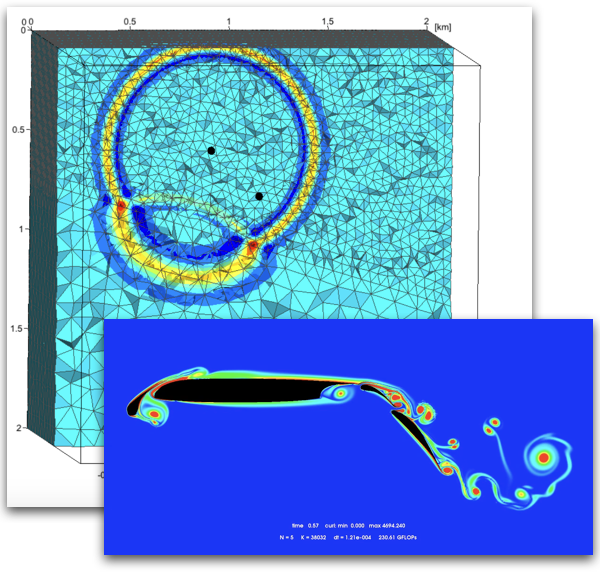
\includegraphics[width=\textwidth]{figs/vortexWave.png}
%\hspace{-.25em}\hbox{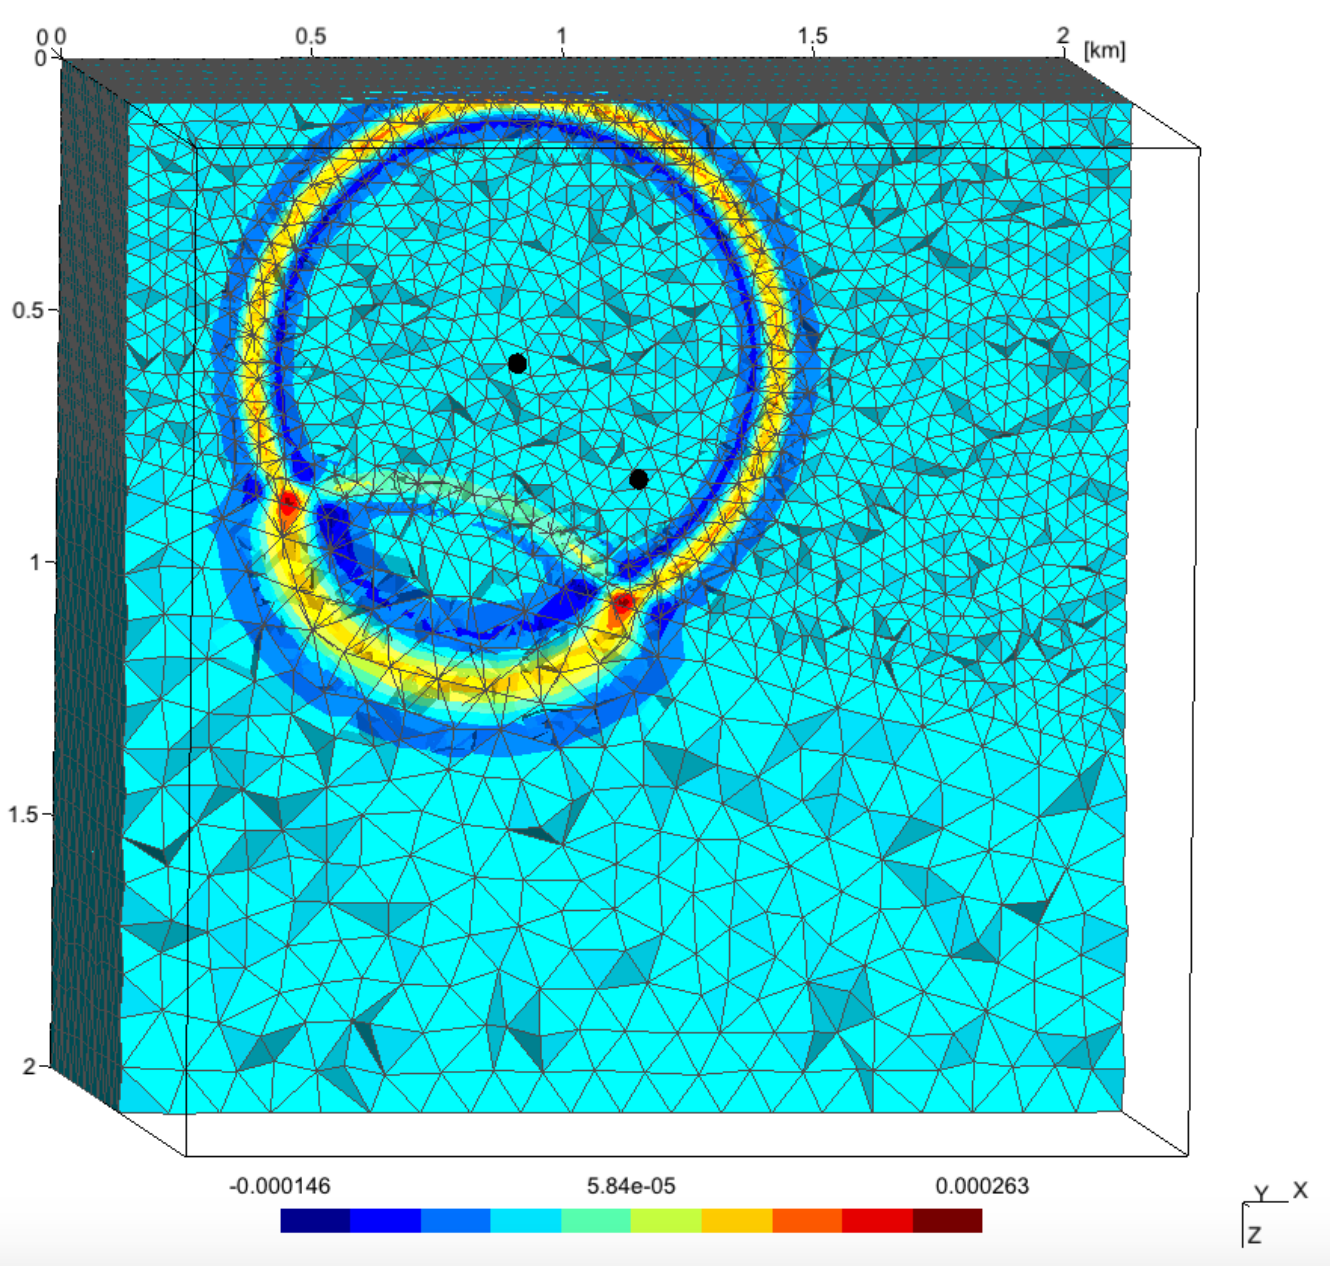
\includegraphics[width=.825\textwidth]{figs/wave.png}}\\
%\vspace{-5.5em}
%\hspace{10em}\hbox{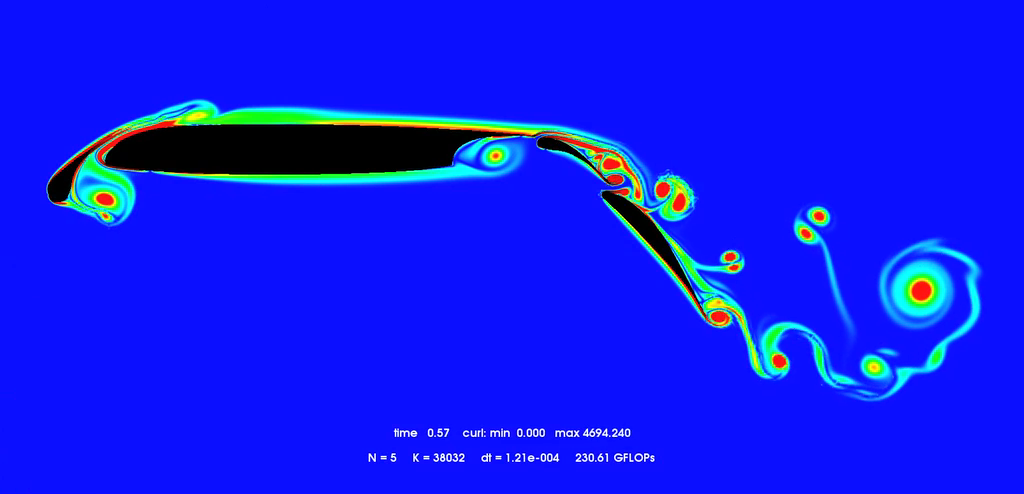
\includegraphics[width=.825\textwidth]{figs/wingflow.png}}
\caption*{\tiny Figures courtesy of T.\ Warburton, A.\ Modave.}
}
\only<2>{
\includegraphics[width=.95\textwidth]{figs/wave_N1.eps}
\caption*{\textbf{Fine} linear approximation.}
}
\only<3>{
\includegraphics[width=.95\textwidth]{figs/wave_N2.eps}
\caption*{\textbf{Coarse} quadratic approximation.}
}
\only<4-5>{
\vspace{1em}
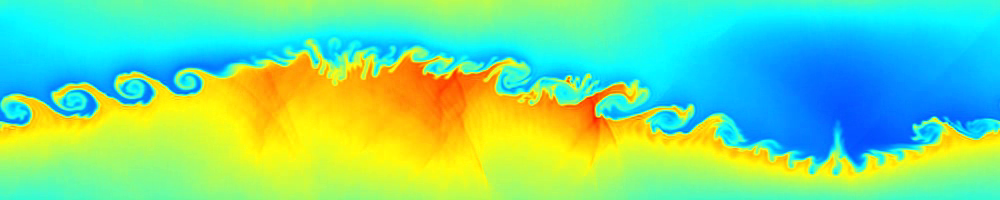
\includegraphics[width=.975\textwidth]{figs/turbulent1.png}\\
\vspace{.5em}
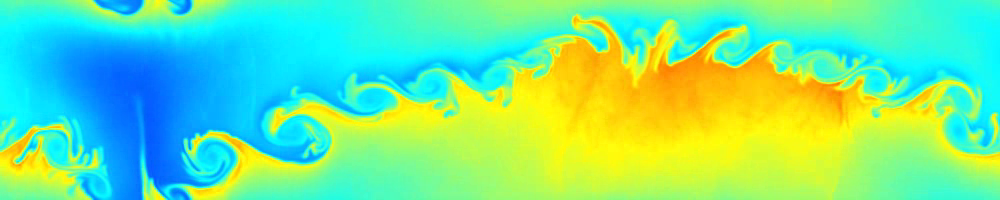
\includegraphics[width=.975\textwidth]{figs/turbulent2.png}
\caption*{\tiny Figure from Per-Olof Persson.}
}
\only<6->{
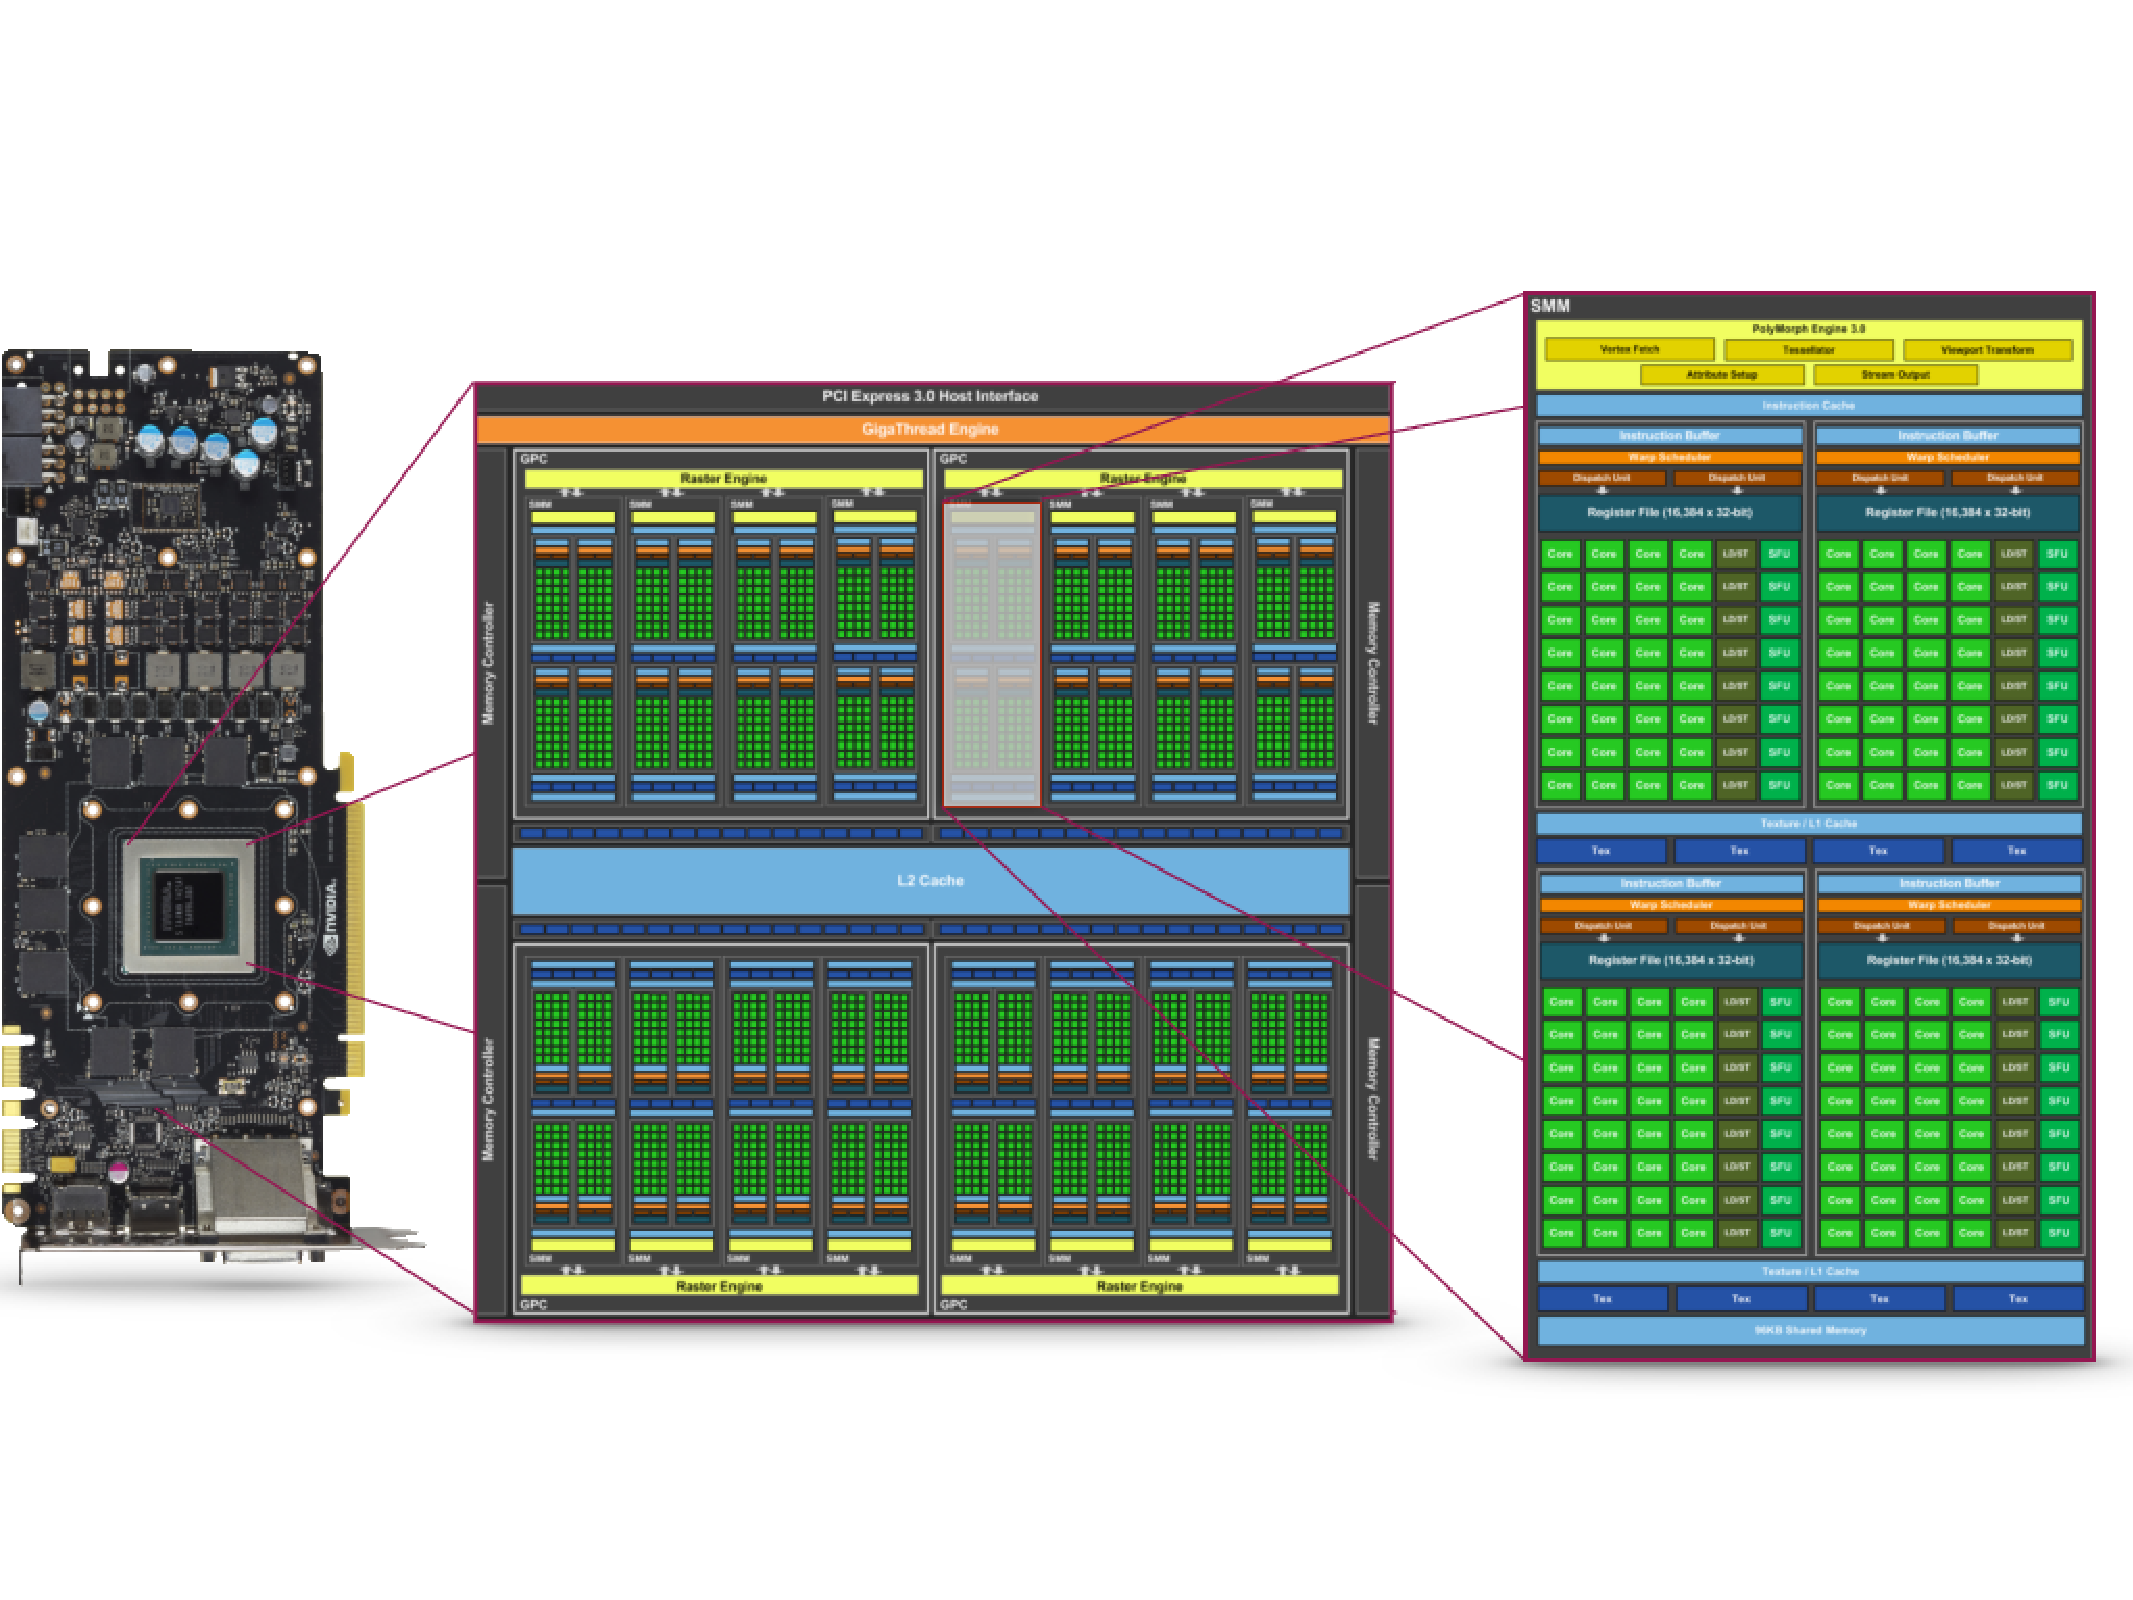
\includegraphics[width=.975\textwidth]{figs/gpu.pdf}
\caption*{A graphics processing unit (GPU).}
}
%\caption*{Image courtesy of Axel Modave.}
\end{overlayarea}
\end{figure}
\end{column}
\end{columns}
%\vspace{1.5em}
%\uncover<7>{
%\begin{center}
%\ovalbox{Goal: address the \note{stability} of efficient high order methods.}
%\end{center}
%}
\end{overlayarea}

%\visible<1>{\let\thefootnote\relax\footnotetext[1]{\tiny Figures courtesy of T.\ Warburton, A.\ Modave.}}
%\visible<5>{\let\thefootnote\relax\footnotetext[5]{\tiny Figure courtesy of T.\ Warburton, Nvidia.}}
}

\frame{
\frametitle{What is considered ``high order''?  Waves vs CFD}
%\vspace{-.5em}
\begin{columns}
\begin{column}{.4\textwidth}
\begin{figure}
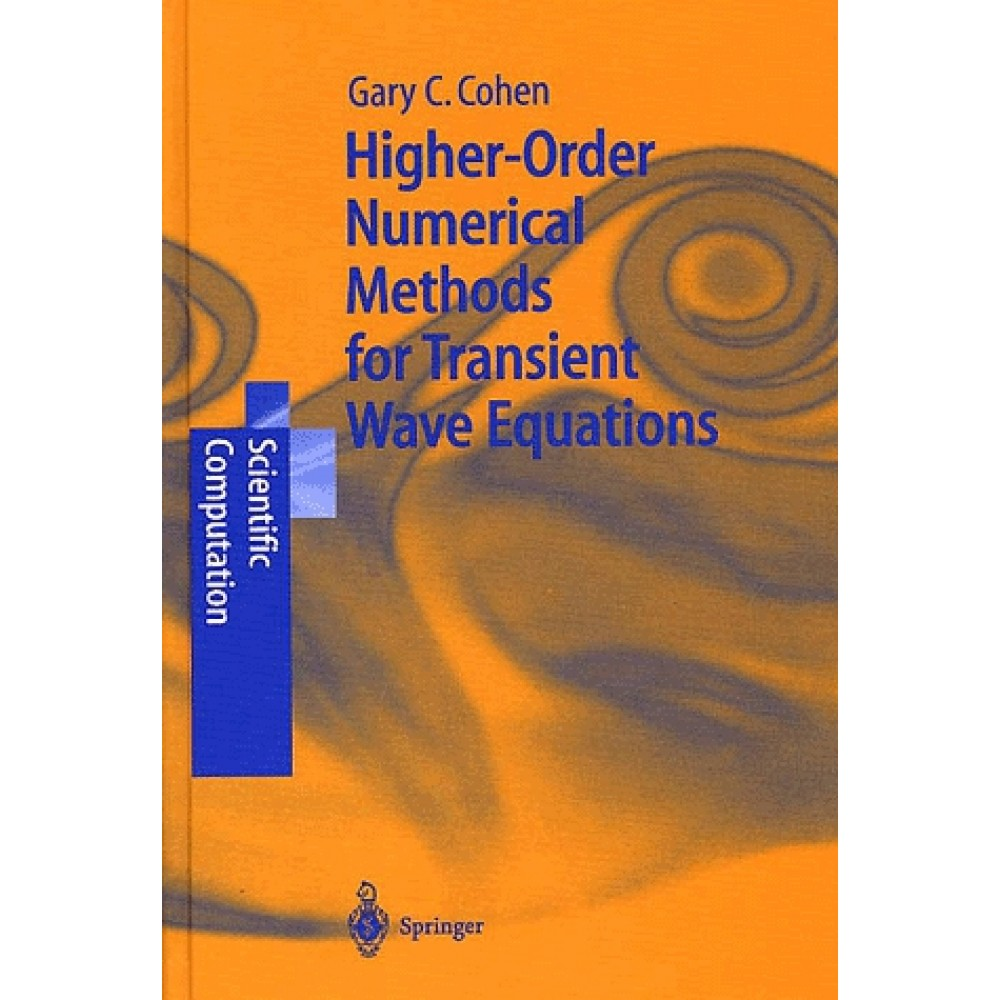
\includegraphics[width=.9\textwidth]{figs/cohenbook.jpg}
\end{figure}
\end{column}
\begin{column}{.6\textwidth}
\begin{itemize}
%\item Spectral and $hp$ finite element methods in the 80s
\item Stability for time-dependent waves, incompressible flow: well established, independent of degree of approx.\ $N$.  
\vspace{.5em}
\item High order for waves: $N = 8, 9, 10$ not uncommon (up to $N \approx 20$).  
\vspace{.5em}
\item High order for CFD: $N > 1$ (considered much less robust than low order!)
\end{itemize}
\end{column}
\end{columns}

\begin{center}
\minibox[frame]{Goal: address robustness of efficient high order methods\\
for time-dependent systems of nonlinear conservation laws.}
\end{center}

%\let\thefootnote\relax\footnotetext{\tiny Chan, Warburton (2017). \emph{GPU-accelerated Bernstein--Bezier DG methods for wave problems}}
\let\thefootnote\relax\footnotetext{\tiny Wang, Fidkowski, Abgrall, Bassi, Caraeni, Cary, Deconinck, Hartmann, Hillewaert, Huynh, and Kroll (2013). \emph{High-order CFD methods: current status and perspective}.}
%\let\thefootnote\relax\footnotetext{\tiny Chan, Demkowicz, and Moser (2014). \emph{A DPG method for steady viscous compressible flow}.}
}

%% =================================================

%\section{High order time-domain DG methods}

%\frame[noframenumbering]{
%\frametitle{Talk outline}
%\tableofcontents
%}
%
%\frame[noframenumbering]{
%\frametitle{Talk outline}
%\tableofcontents[currentsection]
%}

%% =================================================

%\frame{
%\frametitle{Discretizing the PDE: choosing a numerical method}
%%Choose what you want --- for example, I would like:
%%% FD
%\begin{minipage}{\textwidth}
%\begin{minipage}{.5\textwidth}
%Finite difference methods:
%\begin{itemize}
%\item \textcolor{red}{(Block) structured meshes.}
%\item Stencil size grows with order\\of accuracy.
%\end{itemize}
%\end{minipage}
%\begin{minipage}{.5\textwidth}
%\begin{figure}
%\centering
%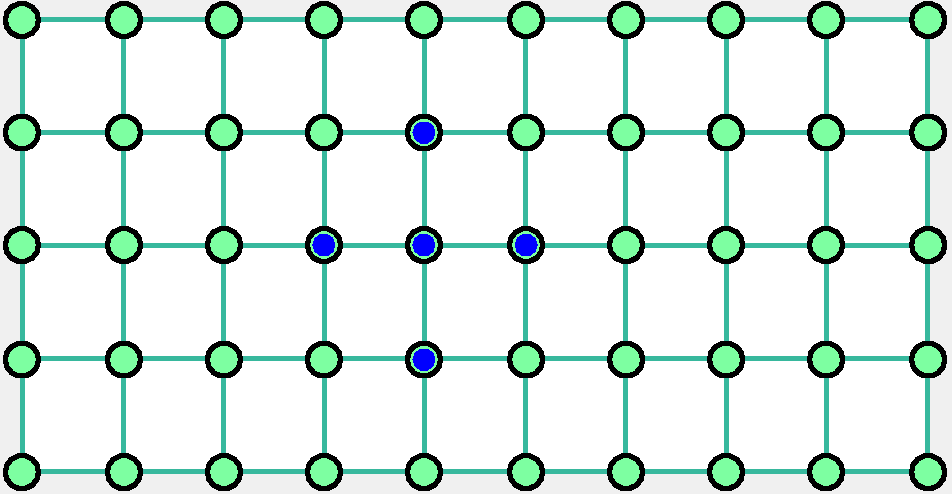
\includegraphics[width=.8\textwidth]{figs/finite_diff.pdf}
%\end{figure}
%\end{minipage}
%\end{minipage}
%
%\vspace{.5em}
%%% FV
%\begin{minipage}{\textwidth}
%\begin{minipage}{.5\textwidth}
%Finite volume methods:
%\begin{itemize}
%\item Complex geometries: unstructured meshes.
%\item \textcolor{red}{Typically low order accurate.}
%\end{itemize}
%
%\end{minipage}
%\begin{minipage}{.5\textwidth}
%\begin{figure}
%\centering
%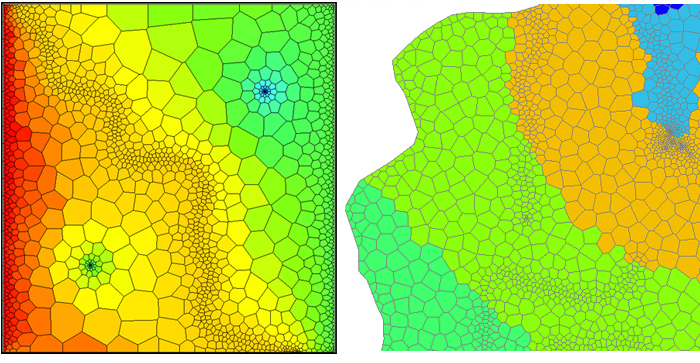
\includegraphics[width=.8\textwidth]{figs/finite_volume.png}
%\end{figure}
%\end{minipage}
%\end{minipage}
%
%\vspace{1em}
%Goals: 
%\begin{itemize}
%\item Flexibility: approximation of solution over complex geometries.
%\item Accuracy: high order methods (mesh size $h$, error $\propto h^{N+1}$). 
%\end{itemize}
%
%\let\thefootnote\relax\footnotetext{\tiny http://www.novametrixgm.com/graphics/blog/finite-volume-method.jpg}
%}
%

%\frame{
%\frametitle{Finite element methods}
%
%\vspace{-.75em}
%\begin{overlayarea}{\textwidth}{\textheight}
%%\vspace{-1em}
%%% FEM
%\begin{columns}
%\begin{column}{.65\textwidth}
%Finite element methods (FEM):
%\vspace{.5em}
%\begin{itemize}
%\item Unstructured meshes.
%\vspace{.5em}
%\item Continuous piecewise polynomial approximation.
%\end{itemize}
%\end{column}
%
%\begin{column}{.35\textwidth}
%\begin{figure}
%\centering
%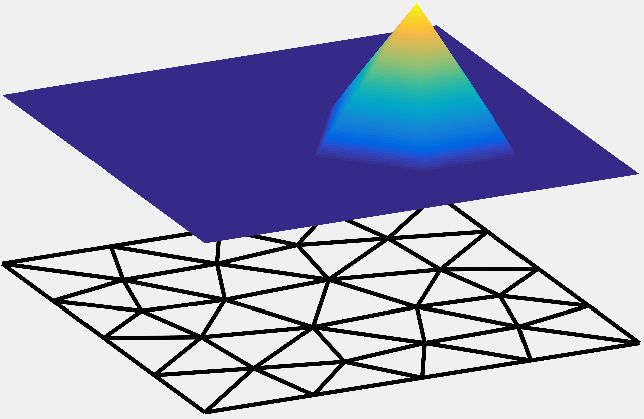
\includegraphics[width=\textwidth]{figs/cg.pdf}
%\end{figure}
%\end{column}
%\end{columns}
%
%\only<1>{
%\vspace{.5em}
%\begin{itemize}
%\item Continuous PDE (example: advection)
%\[
%\pd{u}{t}{} = \pd{u}{x}{}%\div \mathbf{F}(u).
%\]
%\item FEM weak form over domain $\Omega$
%\[
%\int_{\Omega}\pd{u}{t}{} \phi = \int_{\Omega}{\pd{u}{x}{}\phi}, \quad u,\phi \in V_h
%\]
%\end{itemize}
%}
%\only<2>{
%\vspace{-.5em}
%\begin{columns}
%\begin{column}{.65\textwidth}
%FEM yields system of ODEs with\\global mass matrix $\mathbf{M}_{\Omega}$, discretization matrix $\mathbf{A}$.
%\[
%\mathbf{M}_{\Omega}\td{\mathbf{u}}{t} = \mathbf{A}\mathbf{u}.%, \qquad \LRp{\mathbf{M}_{\Omega}}_{ij} = \int_{\Omega} \phi_j\phi_i.
%\]
%FEM mass matrix is \textcolor{red}{globally coupled.}
%\end{column}
%\begin{column}{.35\textwidth}
%\begin{figure}
%\centering
%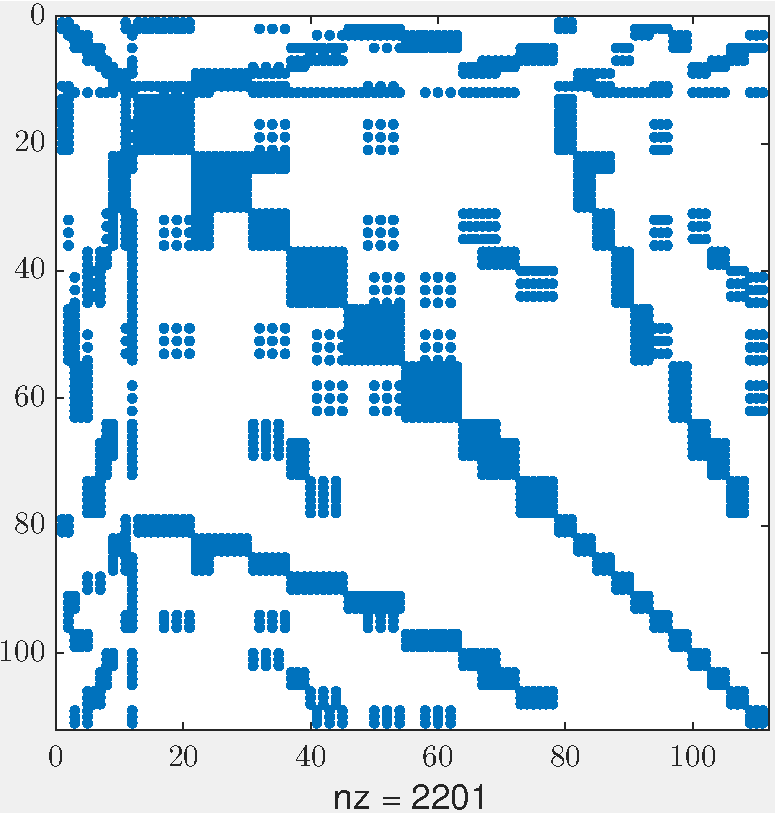
\includegraphics[width=\textwidth]{figs/MCG.pdf}
%%\caption*{\scriptsize Globally coupled FEM mass matrix.}
%\end{figure}
%\end{column}
%\end{columns}
%}
%\end{overlayarea}
%}

\section{Stability of DG: simple problems vs nonlinear conservation laws} 


\frame[noframenumbering]{
\frametitle{Talk outline}
\tableofcontents
}

\frame[noframenumbering]{
\frametitle{Talk outline}
\tableofcontents[currentsection]
}



\frame{
\frametitle{Discontinuous Galerkin methods}

\vspace{-.75em}
\begin{overlayarea}{\textwidth}{\textheight}
\begin{columns}
\begin{column}{.65\textwidth}
Discontinuous Galerkin (DG) methods: 
\vspace{.5em}
\begin{itemize}
\item High order accuracy, geometric flexibility.
\vspace{.5em}
\item Weak continuity across faces.
\end{itemize}
\end{column}

\begin{column}{.35\textwidth}
\vspace{-.5em}
\begin{figure}
\centering
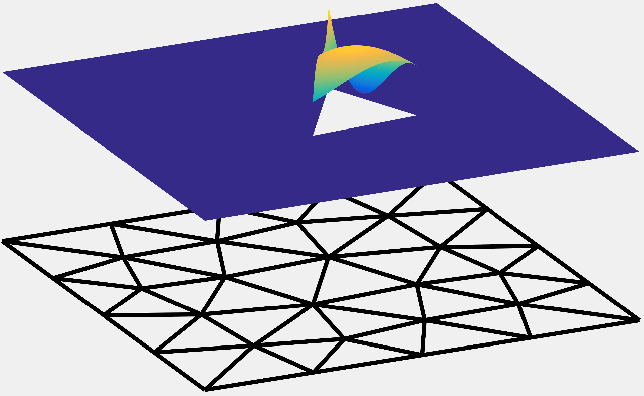
\includegraphics[width=\textwidth]{figs/dg.pdf}
\end{figure}
\end{column}
\end{columns}

\only<1>{
\vspace{.5em}
\begin{itemize}
\item Continuous PDE (example: advection)
\[
\pd{u}{t}{} = \pd{f(u)}{x}{}, \qquad f(u) = u.
\]
\item Local DG form with numerical flux $\bm{f}^*$: find $u \in P^N\LRp{D^k}$ such that
\[
\int_{D_k}\pd{u}{t}{} \phi = \int_{D_k}\pd{f(u)}{x}{}\phi + \int_{\partial D_k}{\bm{n}\cdot\LRp{\bm{f}^*-\bm{f}(u)}\phi}, \qquad \forall \phi \in P^N\LRp{D^k}.
\]
\end{itemize}
}
\only<2>{
\vspace{-.5em}
\begin{columns}
\begin{column}{.65\textwidth}
DG in space yields system of ODEs %with\\global mass matrix $\mathbf{M}_{\Omega}$, discretization matrix $\mathbf{A}$.
\[
\mathbf{M}_{\Omega}\td{\mathbf{u}}{t} = \mathbf{A}\mathbf{u}. %\qquad \LRp{\mathbf{M}_{\Omega}}_{ij} = \int_{\Omega} \phi_j\phi_i.
\]
DG mass matrix decouples across elements,\\inter-element coupling only through $\mathbf{A}$.
\end{column}
\begin{column}{.35\textwidth}
\vspace{-.33em}
\begin{figure}
\centering
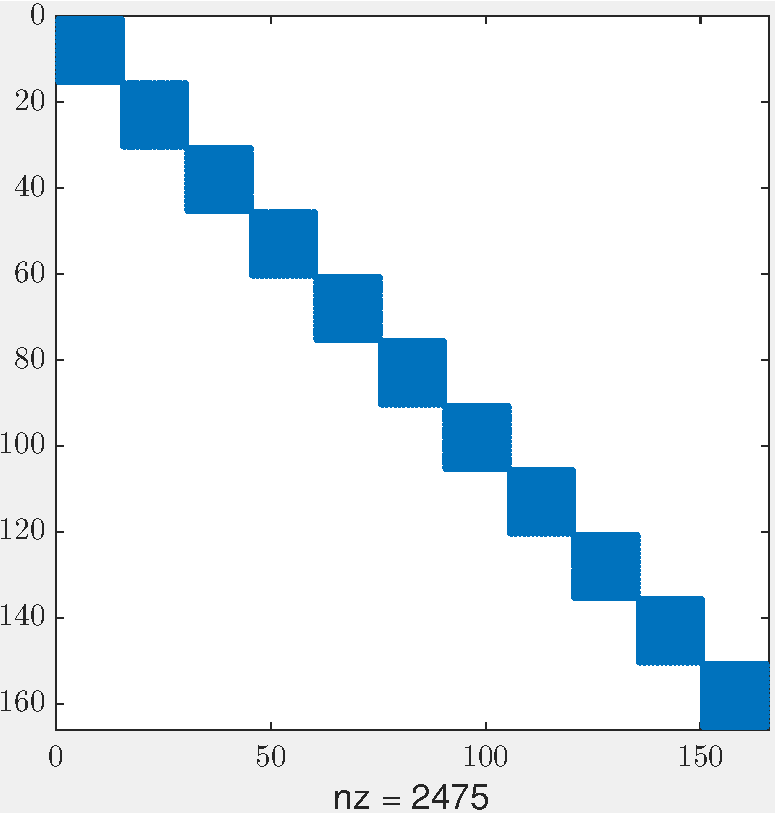
\includegraphics[width=\textwidth]{figs/MDG.pdf}
\vspace{-.33em}
\caption*{\tiny Global mass matrix $\bm{M}_{\Omega}$.}
\end{figure}
\end{column}
\end{columns}
}
\end{overlayarea}
}

%\frame{
%\frametitle{High order nodal discontinuous Galerkin methods}
%\vspace{-.5em}
%\begin{figure}
%\centering
%\subfloat{\includegraphics[width=.24\textwidth]{figs/nodal1D.eps}}
%\subfloat{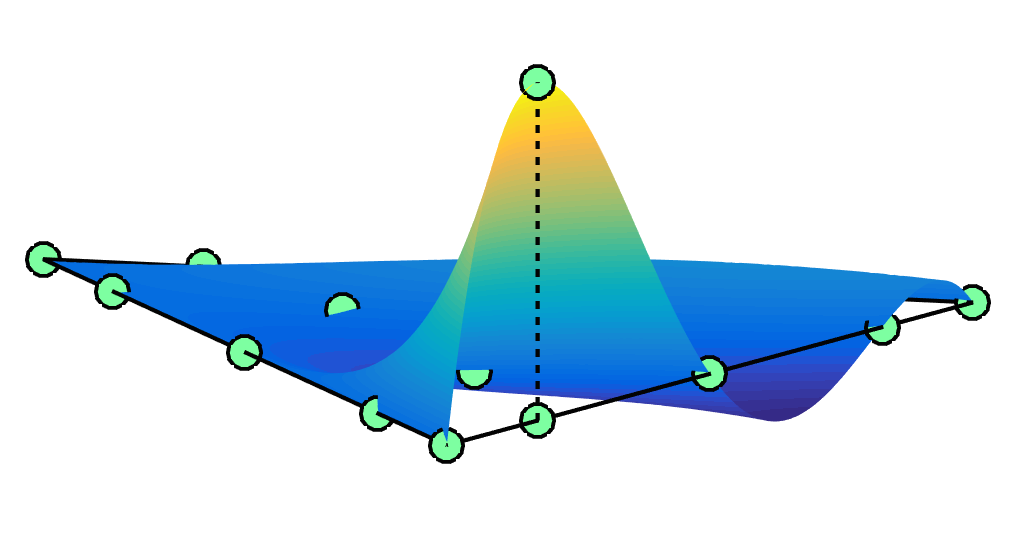
\includegraphics[width=.4\textwidth]{figs/nodal2D.png}}
%\hspace{.1em}
%\subfloat{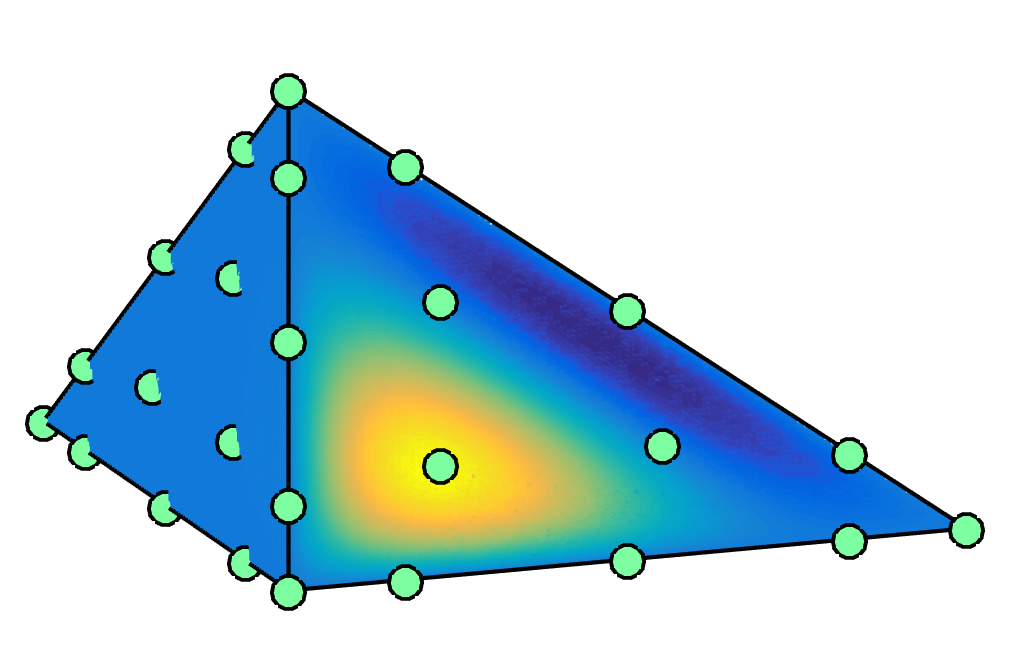
\includegraphics[width=.31\textwidth]{figs/nodal3D.png}}
%\caption*{Lagrange (nodal) bases on a line, triangle, tetrahedron.   }
%\end{figure}
%%\vspace{.5em}
%\begin{itemize}
%\item Nodal bases defined implicitly through an orthogonal basis.  
%\vspace{.5em}
%\item Point locations optimized for interpolation and numerical stability. 
%\vspace{.5em}
%\item Assume \textbf{affine} tetrahedra, coefficients \textbf{constant} on each element.
%%\item Derivative matrices w.r.t.\ reference coordinates $\bm{\widehat{x}} = (r,s,t)$ 
%%\[
%%\LRp{\mathbf{\widehat{D}}_r}_{ij} = \pd{\ell_j(\bm{\widehat{x}}_i)}{r}{}, \qquad \LRp{\mathbf{\widehat{D}}_s}_{ij} = \pd{\ell_j(\bm{\widehat{x}}_i)}{s}{}, \qquad \LRp{\mathbf{\widehat{D}}_t}_{ij} = \pd{\ell_j(\bm{\widehat{x}}_i)}{t}{}.
%%\]
%\end{itemize}
%}

\frame{
\frametitle{Time-domain explicit DG methods}
%\vspace{-2em}
\begin{columns}
\begin{column}{.55\textwidth}
Given initial condition $u(\mathbf{x},0)$:
\vspace{.25em}
\begin{itemize}
\item<1-> Compute numerical flux on\\element faces (\textcolor{red}{non-local}).
\vspace{.25em}
\item<2-> Compute RHS of (\textcolor{blue}{local}) ODE.%: differentiation and lifting matrices.
\vspace{.25em}
\item<3-> Evolve  (\textcolor{blue}{local}) solution using \textcolor{red}{explicit} time integration (RK, AB, etc). 
\end{itemize}
\end{column}
\begin{column}{.45\textwidth}
\begin{figure}
\centering
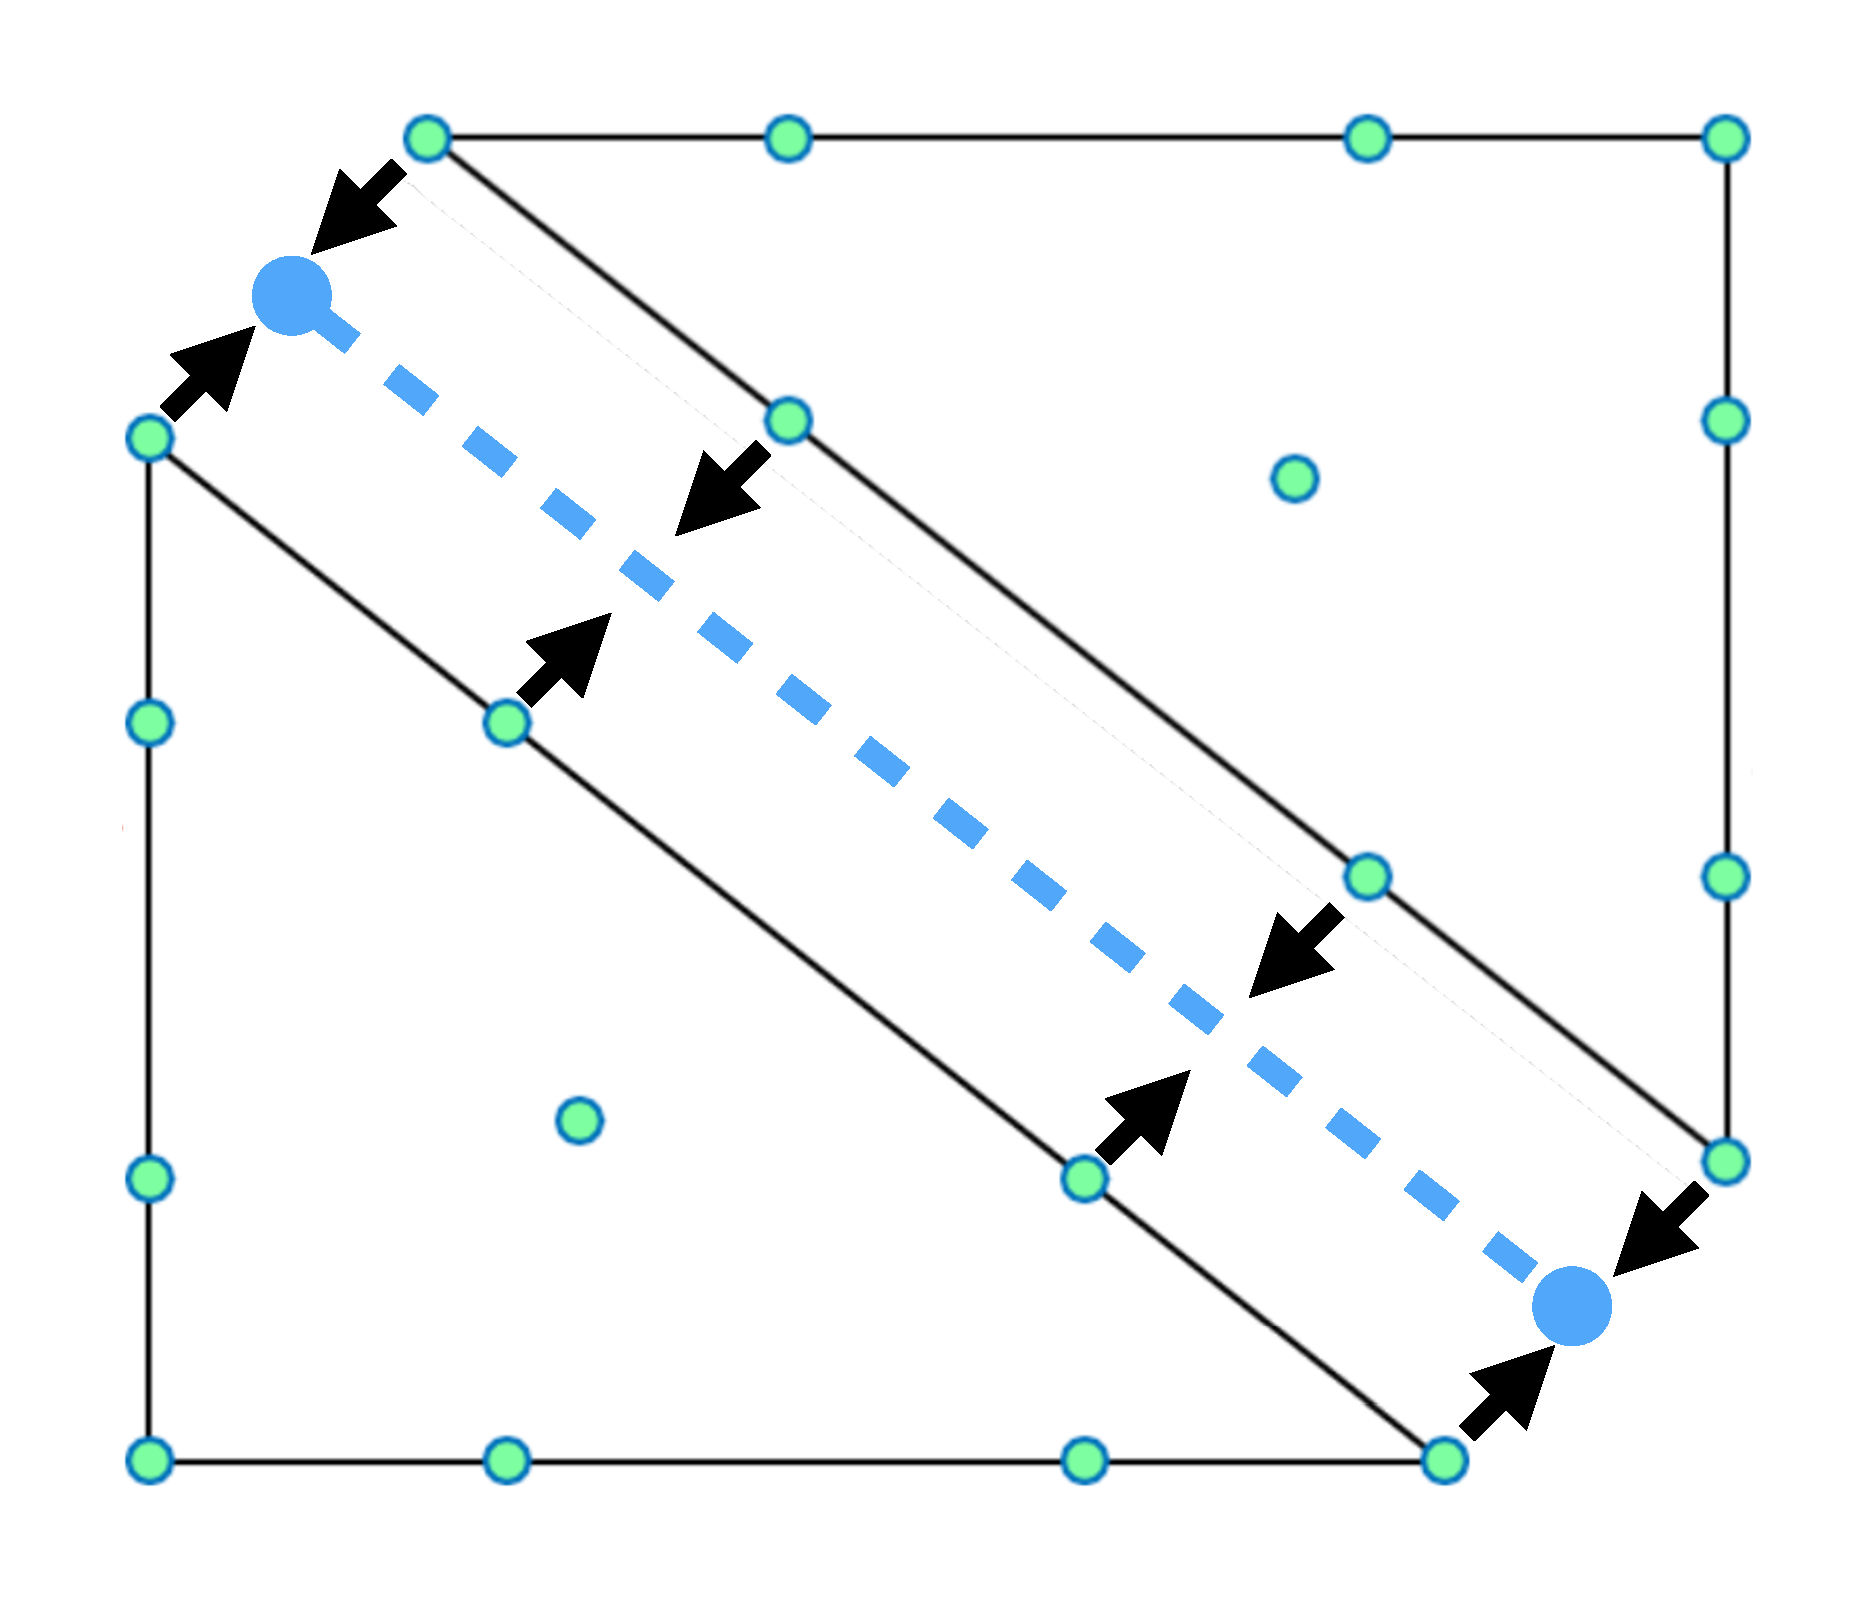
\includegraphics[width=.85\textwidth]{figs/nodal.pdf}
\end{figure}
\end{column}
\end{columns}
%\vspace{1em}
\begin{overlayarea}{\textwidth}{.4\textheight}
\only<1>{\[
\td{\mathbf{u}}{t} = \mathbf{D}_x \mathbf{u} + \sum_{\text{ faces}}\mathbf{L}_f \LRp{\rm \textcolor{red}{flux}}, \qquad \mathbf{L}_f = \mathbf{{M}}^{-1}\mathbf{{M}}_f.
\]
}
\only<2>{
\[
\td{\mathbf{u}}{t} = \underbrace{\mathbf{D}_x \mathbf{u}}_{\text{\textcolor{blue}{Volume}}} + \underbrace{\sum_{\text{ faces}}\mathbf{L}_f \LRp{\rm \textcolor{red}{flux}}}_{\text{\textcolor{blue}{Surface}}}, \qquad \mathbf{L}_f = \mathbf{{M}}^{-1}\mathbf{{M}}_f.
\]
}
\only<3>{
\[
\underbrace{\td{\mathbf{u}}{t}}_{\text{\textcolor{blue}{Update}}} = \underbrace{\mathbf{D}_x \mathbf{u}}_{\text{\textcolor{blue}{Volume}}} + \underbrace{\sum_{\text{ faces}}\mathbf{L}_f \LRp{\rm \textcolor{red}{flux}}}_{\text{\textcolor{blue}{Surface}}}, \qquad \mathbf{L}_f = \mathbf{{M}}^{-1}\mathbf{{M}}_f.
\]
}
\only<4>{
\vspace{.5em}
\begin{center}
\textbf{Pros:} simple, scalable, and efficient matrix-free implementation. 
\\
\vspace{.5em}
\textbf{Cons:} explicit and high order methods: both prone to \textcolor{red}{instability}.\\
Regularization (slope limiting, artificial viscosity) to avoid blow up!
\\
\vspace{1em}
\ovalbox{Must ensure semi-discrete system is inherently \emph{energy stable}!}
\end{center}
}
\end{overlayarea}

}% frame


\frame{
\frametitle{Semi-discrete energy stability of DG methods}

\begin{itemize}
\item<1-> Linear periodic advection on $[-1,1]$
\[
\pd{u}{t} + \pd{u}{x} = 0, \qquad u(-1) = u(1), \qquad \Longrightarrow \pd{}{t}\nor{u}_{L^2([-1,1])}^2 = 0.  
\]
\item<2-> Triangulate domain with elements $D^k$, define $\jump{u} = u^+ - u$ on $D^k$.
\vspace{.5em}
\item<2-> DG formulation: find $u(x) \in P^N(D^k)$ s.t.\ $\forall v \in P^N(D^k)$
\begin{align*}
%\sum_k 
\sum_{k} \int_{D^k} \LRp{\pd{u}{t} + \pd{u}{x}}v \diff{x} + 
\frac{1}{2}\int_{\partial D^k}\LRp{\jump{u}n_x + \tau\jump{u}}v \diff{x}=0.
%\sum_k\int_{D^k} \LRp{\pd{u}{t} + \pd{u}{x}}v + 
%\int_{\partial D^k} \frac{n_x-\tau\LRb{n_x}}{2} \jump{u}v  = 0, \qquad \forall v \in V_h.
\end{align*}
\item<3-> Energy estimate: take $v = u$, chain rule in time, \textcolor{red}{integrate by parts}.  
\begin{align*}
\sum_k \pd{}{t} \nor{u}_{D^k}^2  \leq -\sum_k \frac{\tau}{2}\int_{\partial D^k}\jump{u}^2 \diff{x}.
%\sum_k\int_{D^k} \LRp{\pd{u}{t} + \pd{u}{x}}v + 
%\int_{\partial D^k} \frac{n_x-\tau\LRb{n_x}}{2} \jump{u}v  = 0, \qquad \forall v \in V_h.
\end{align*}

\end{itemize}
%\vspace{-.5em}
}

\frame{
\frametitle{Energy conservative and energy stable DG methods}
%\begin{overlayarea}{\textwidth}{.475\textheight}
\begin{itemize}
\item Energy estimate: implies solution is non-increasing if $\tau \geq 0$.
\vspace{.25em}
\item Energy conservative ``central'' flux when $\tau = 0$.
\vspace{.25em}
\item Energy stable (i.e. dissipative) ``Lax-Friedrichs'' flux when $\tau = 1$.
\end{itemize} 
\begin{figure}
\centering
\captionsetup[subfloat]{width=.5\textwidth, justification=centering}
\subfloat[Energy conservative ($\tau = 0$)]{
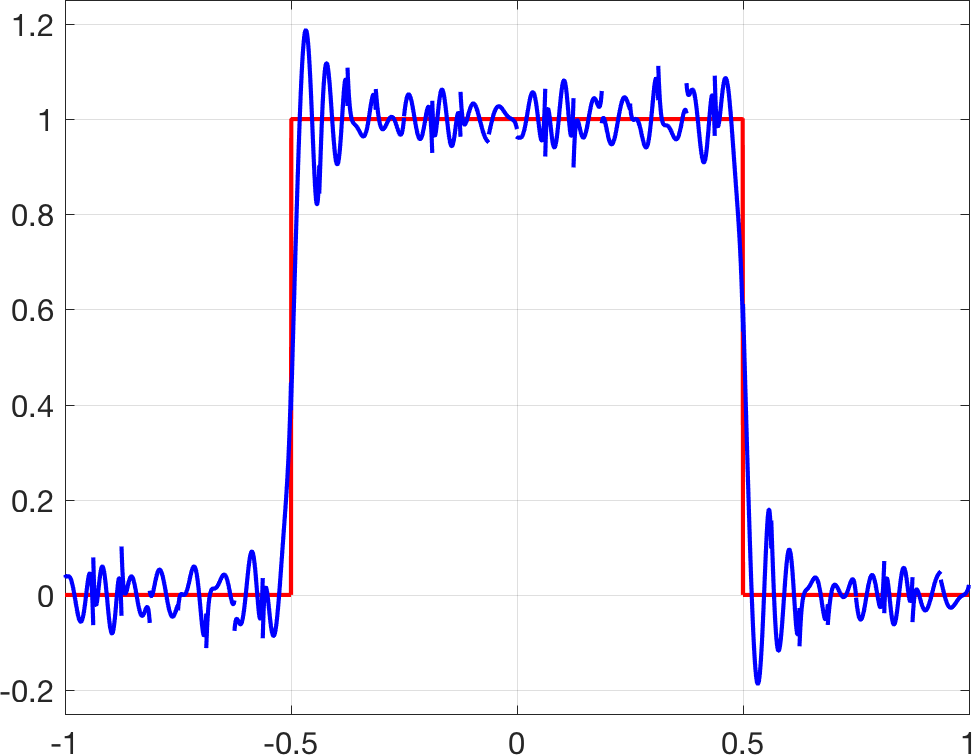
\includegraphics[width=.425\textwidth]{figs/advecCentral.png}}
\hspace{.5em}
\subfloat[Energy stable ($\tau = 1$)]{
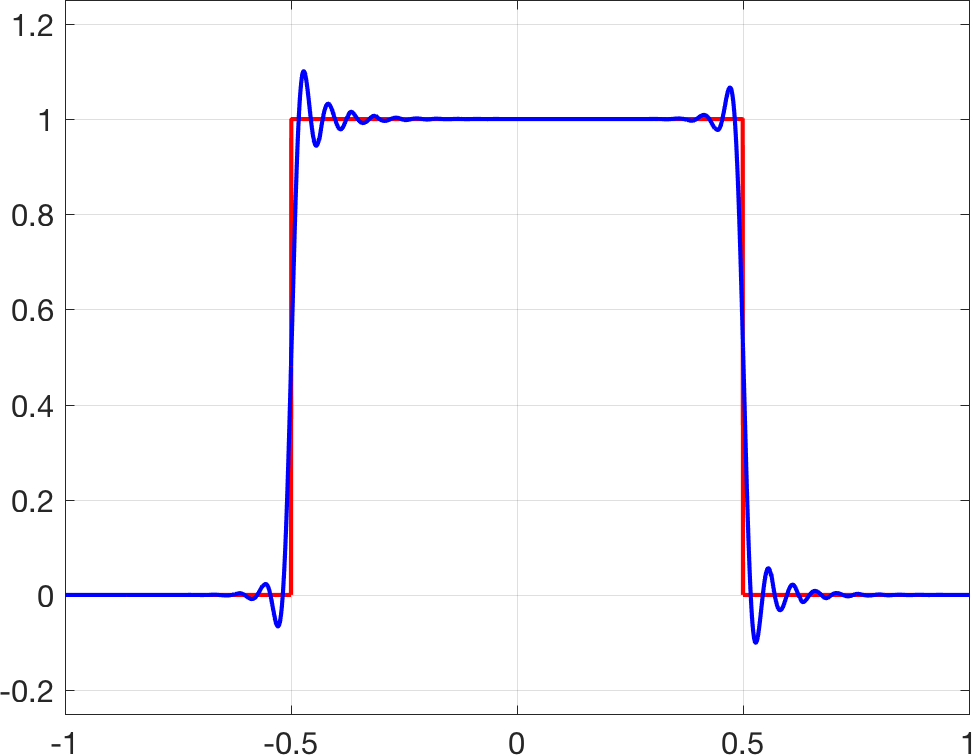
\includegraphics[width=.425\textwidth]{figs/advecUpwind.png}}
\end{figure}
%\end{overlayarea}
}

%% =================================================

%\frame{
%\frametitle{Global DG differentiation operators}
%
%\begin{overlayarea}{\textwidth}{.95\textheight}
%\begin{itemize}
%\item<1-> Let $V_h = \bigoplus_k P^N(D^k)$.  Define jump, average across shared face
%\[
%\jump{u} = u^+ - u, \qquad \avg{u} = \frac{u^+ + u}{2}, \qquad u^+ = u \text{ on boundary}.
%\]
%\only<1>{
%\vspace{-.5em}
%\begin{figure}
%%\centering
%\hspace{-3em}\hbox{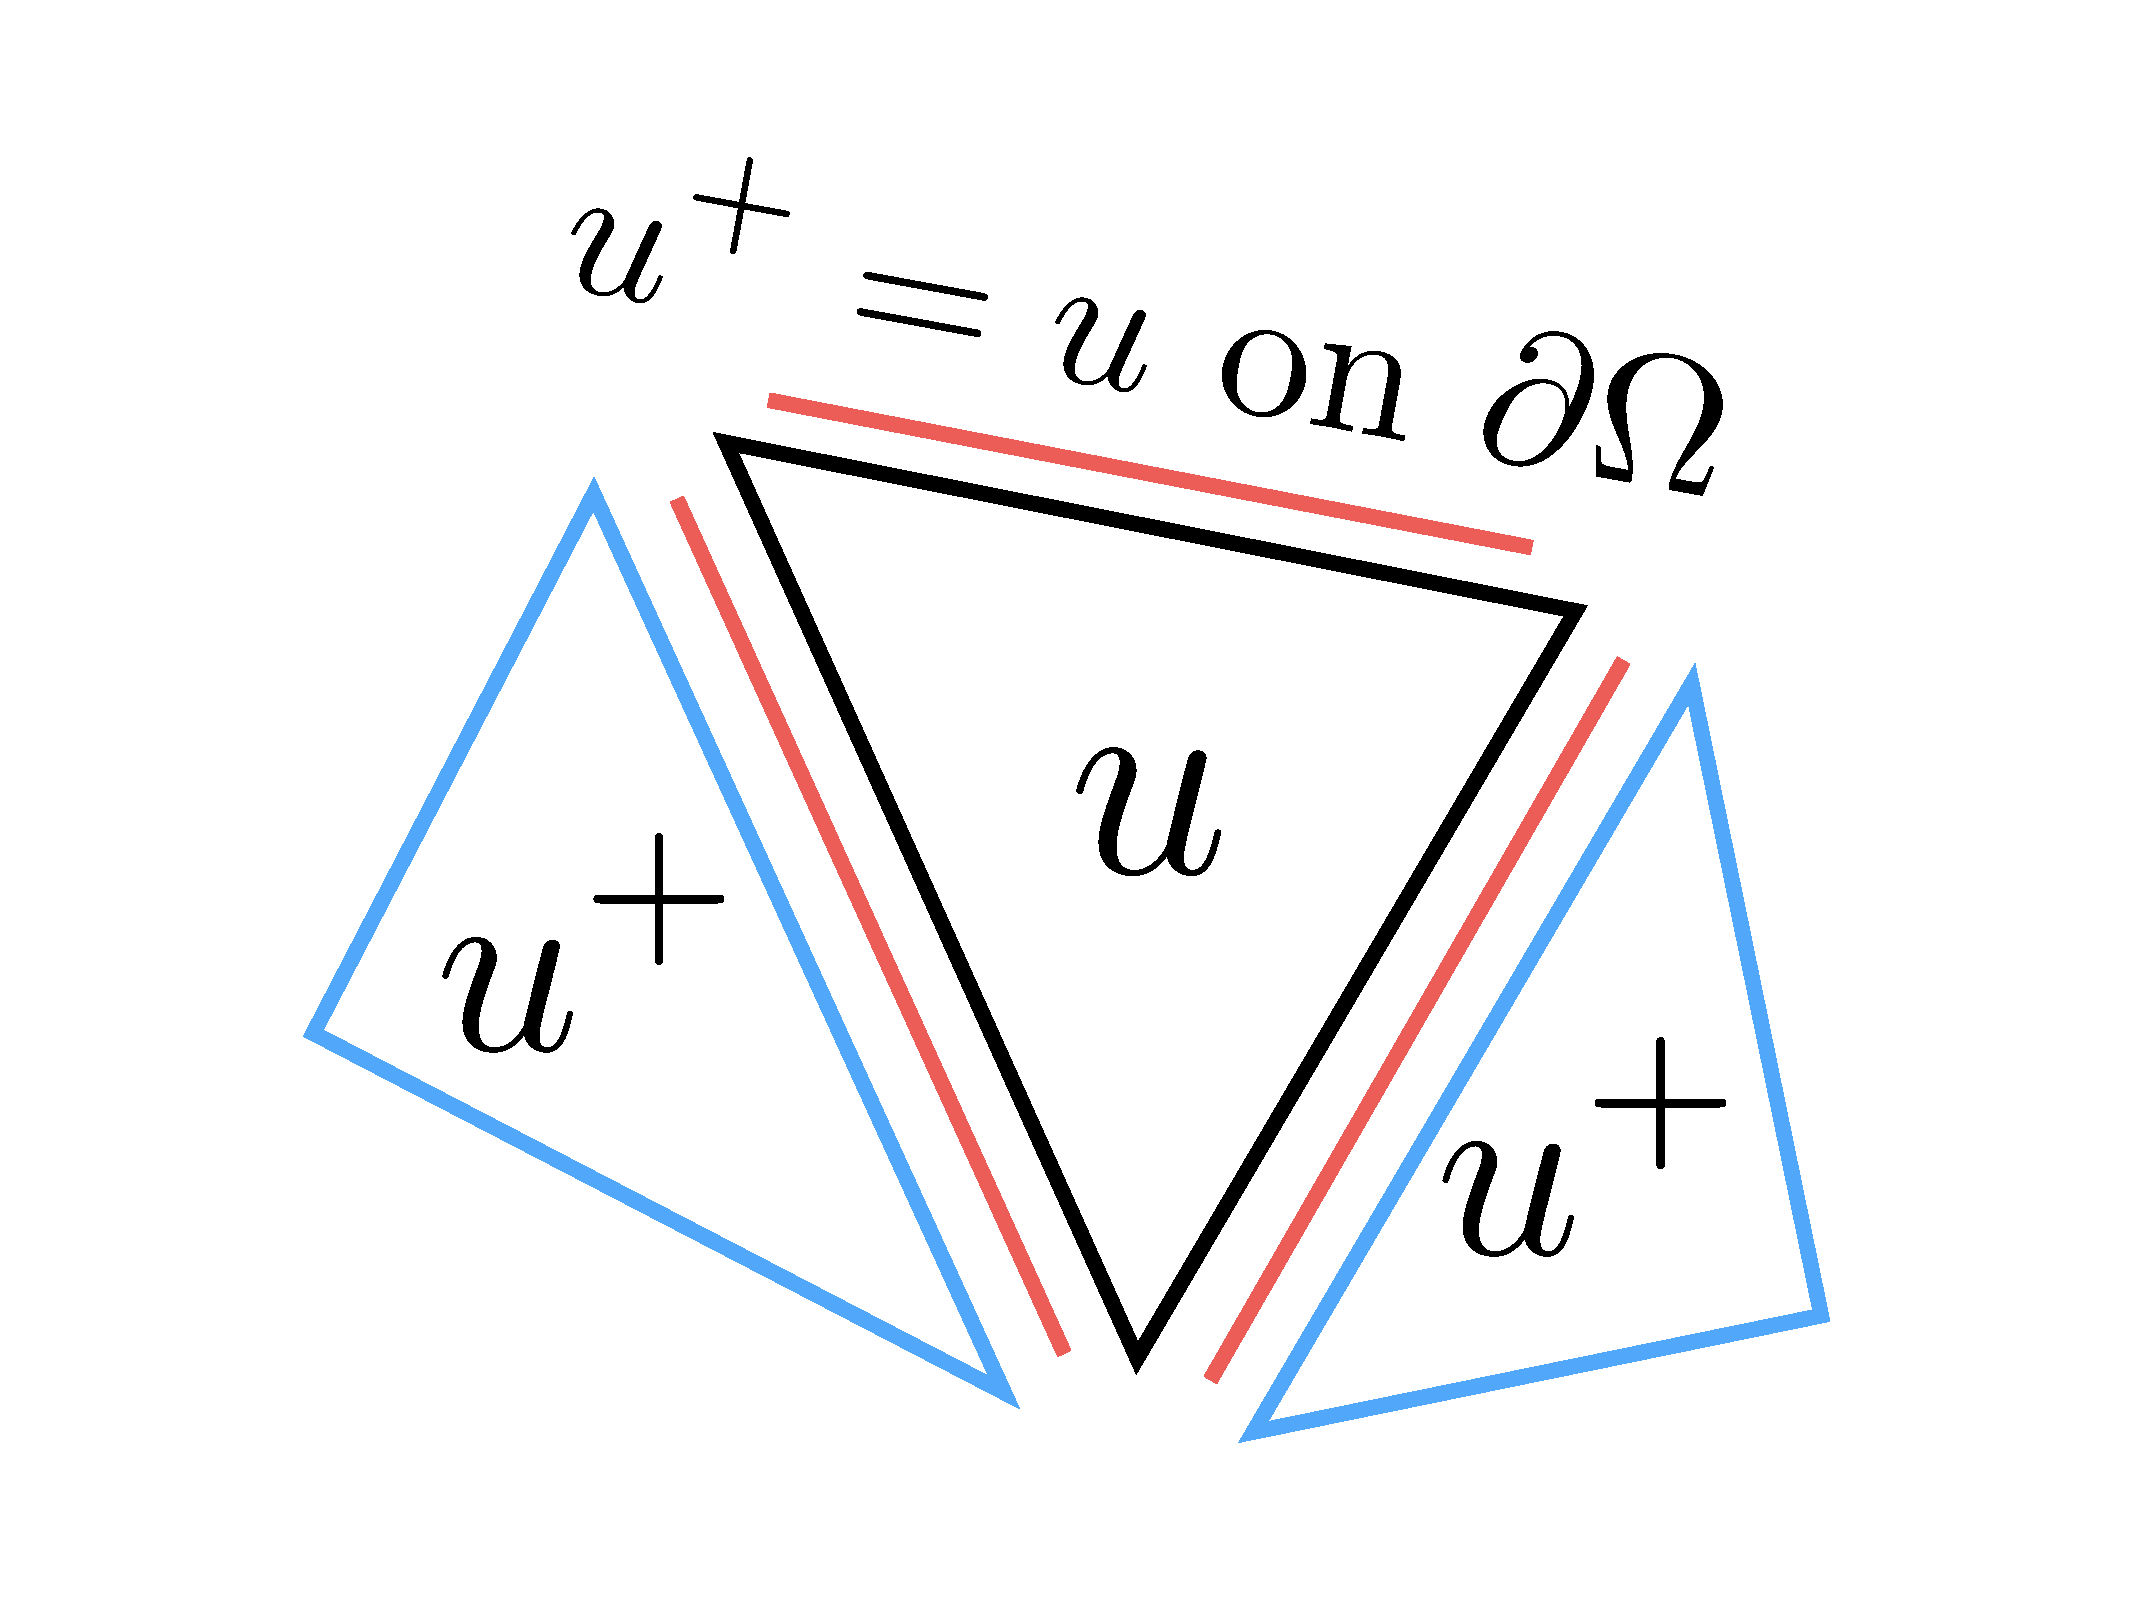
\includegraphics[width=.475\textwidth]{figs/jumpAvg.pdf}}
%\end{figure}
%}
%\only<2->{
%\item<2-> Affine meshes: define \note{global} DG derivative $D^x_h: V_h \rightarrow V_h$: $\forall v\in V_h$, 
%\begin{align*}
%\LRp{D^x_h u,v}_{\Omega} &= \sum_{k} \LRp{-u,\pd{v}{x}}_{D^k} + \LRa{\avg{u},vn_x}_{\partial D^k},\\ 
%&= \sum_{k} \LRp{\pd{u}{x},v}_{D^k} + \frac{1}{2}\LRa{\jump{u},vn_x}_{\partial D^k}.  
%\end{align*}
%\item<3-> Global integration by parts: {holds for quadrature (degree $\geq 2N-1$)}. 
%\[
%\LRp{D^x_h u,v}_{\Omega} = \LRa{ u,v n_x}_{\partial \Omega} - \LRp{u, D^x_hv}_{\Omega}, \qquad \forall u,v \in V_h.
%\]
%}
%\end{itemize}
%\end{overlayarea}
%}
%
%\frame{
%\frametitle{Global DG differentiation matrices}
%\begin{itemize}
%\item $D^x_h$ a matrix representation
%\item Let $\bm{U} = [\bm{u}_1,\ldots,\bm{u}_K]^T$.  Semi-discrete system: 
%\[
%\td{\bm{U}}{t} = \bm{D}^x_h \bm{U}
%\]
%\end{itemize}
%}
%
%\frame{
%\frametitle{DG energy estimates for linear advection }
%
%\begin{itemize}
%\item Advection formulation: positive semi-definite penalization $s_\tau(u,v)$
%\[
%\LRp{\pd{u}{t} + D^x_h u,v}_{\Omega} + \underbrace{\sum_{k} \LRa{-\tau\frac{\LRb{n_x}}{2} \jump{u},v}_{\partial D^k}}_{s_\tau(u,v) } = 0. %\text{, pos.\ semi-def.}
%\]
%\item Energy method: take $v = u$, integrate by parts.  
%\begin{align*}
%&\LRp{\pd{u}{t},u} + \frac{1}{2}\note{{\LRp{2D^x_h u,u}_{\Omega}}} + s_{\tau}(u,u) = 0.  \\
%&\note{\LRp{2D^x_h u,u}_{\Omega}} = {\LRp{D^x_h u,u}_{\Omega} + \LRa{u,un_x}_{\partial \Omega} - \LRp{u,D^x_h u}_{\Omega}},\\
%&\Longrightarrow \frac{1}{2}\pd{}{t}\nor{u}^2_{L^2\LRp{\Omega}} +  \frac{1}{2}\LRa{u,un_x}_{\partial \Omega} = -s_{\tau}(u,u) \leq 0.
%\end{align*}
%
%\end{itemize}
%}


%% =================================================


\frame{
\frametitle{Entropy stability for nonlinear conservation laws}
\vspace{-.5em}
\begin{itemize}
\item Generalizes energy stability to nonlinear systems of conservation laws (Burgers', shallow water, compressible Euler, MHD).  
\[
\pd{\bm{u}}{t} + \pd{\bm{f}(\bm{u})}{x} = 0.  
\]
\item Continuous entropy inequality: convex \note{entropy} function $S(\bm{u})$ and ``entropy potential'' $\psi(\bm{u})$.  
\begin{align*}
&\int_{\Omega} \bm{v}^T\LRp{\pd{\bm{u}}{t} + \pd{\bm{f}(\bm{u})}{x}} = 0, \qquad \bm{v} = \pd{S}{\bm{u}} \\
&\Longrightarrow \int_{\Omega}\pd{S(\bm{u})}{t} + \LRu{\LRp{\bm{v}^T\bm{f}(\bm{u}) - \psi(\bm{u})}}_{-1}^1 \leq 0.
\end{align*}
\vspace{.01em}
\item Proof of entropy inequality relies on \note{chain rule}, integration by parts.  
\end{itemize}
}

\frame{
\frametitle{Example: mathematical entropy (compressible flow)}

\begin{itemize}
\item Conservative variables: density, momentum, energy
\[
\bm{u} = (\rho, \bm{m}, E), \qquad \rho > 0, \qquad E > \frac{1}{2} {\LRb{\bm{m}}^2}/{\rho}.
\]
\item Physical entropy $s(\bm{u})$ always increasing; \note{mathematical entropy $S(\bm{u})$} always decreasing (analogous to energy).
\[
s(\bm{u}) = \log\LRp{\frac{(\gamma-1) \rho e}{\rho^\gamma}}, \qquad S(\bm{u}) = -\rho s(\bm{u}).
\]
\item Entropy variables $\bm{v}(\bm{u})$: invertible function of $\bm{u}$
\[
\bm{v}(\bm{u}) = \pd{S}{\bm{u}} = \frac{1}{\rho e} \LRp{\begin{array}{c}
\rho e (\gamma + 1 - s(\bm{u})) - E \\
m\\
-\rho
\end{array}}
\]
\end{itemize}
}


\frame{
\frametitle{Why are discretizations of nonlinear PDEs unstable?}
\setcounter{subfigure}{0}
\vspace{-1em}
\begin{figure}
\begin{overprint}
\centering
\foreach \id in {1,2,3,4}{%
\only<\id>{
\captionsetup[subfloat]{width=.45\textwidth, justification=centering}
\subfloat[$N = 7, K = 8$ (aligned mesh)]{
\makebox[.425\textwidth]{\includegraphics[width=.32\textwidth]{figs/burgersStable_\id.png}}}%
\hspace{1em}%
\subfloat[$N = 7, K = 9$ (non-aligned mesh)]{
\makebox[.425\textwidth]{\includegraphics[width=.32\textwidth]{figs/burgersUnstable_\id.png}}}
} % only
} % foreach 
\end{overprint}
\end{figure}
\vspace{-.5em}
\begin{itemize}
\item Burgers' equation: $f(u) = u^2/2$.  How to compute $\pd{}{x}f({u})$?  
\[
\pd{u}{t} + \frac{1}{2}\pd{u^2}{x} = 0, \qquad u \in P^N(D^k), \quad u^2 \not\in P^N(D^k).
\]
\item Differentiating $L^2$ projection $P_N$ + inexact quadrature: \note{no chain rule}.  
\[
\int_{D^k}\LRp{\pd{u}{t} + \frac{1}{2} \pd{}{x} P_N u^2}v \diff{x} = 0, \qquad \frac{1}{2}\pd{P_N u^2}{x} \neq P_N \LRp{u \pd{u}{x}}
\]
\end{itemize}
}

\frame{
\frametitle{Tradeoff: high order accuracy vs stability}

\begin{overlayarea}{\textwidth}{.85\textheight}
\begin{itemize}
\item<1-> \textcolor{red}{Asymptotic} stability for \textcolor{red}{smooth} solutions (not shocks or turbulence!)
\item<3-> One option: \note{stabilize by regularizing} (limiters, filtering, art.\ viscosity).  
\end{itemize}
\begin{figure}
\centering
\only<1>{
\vspace{.5em}
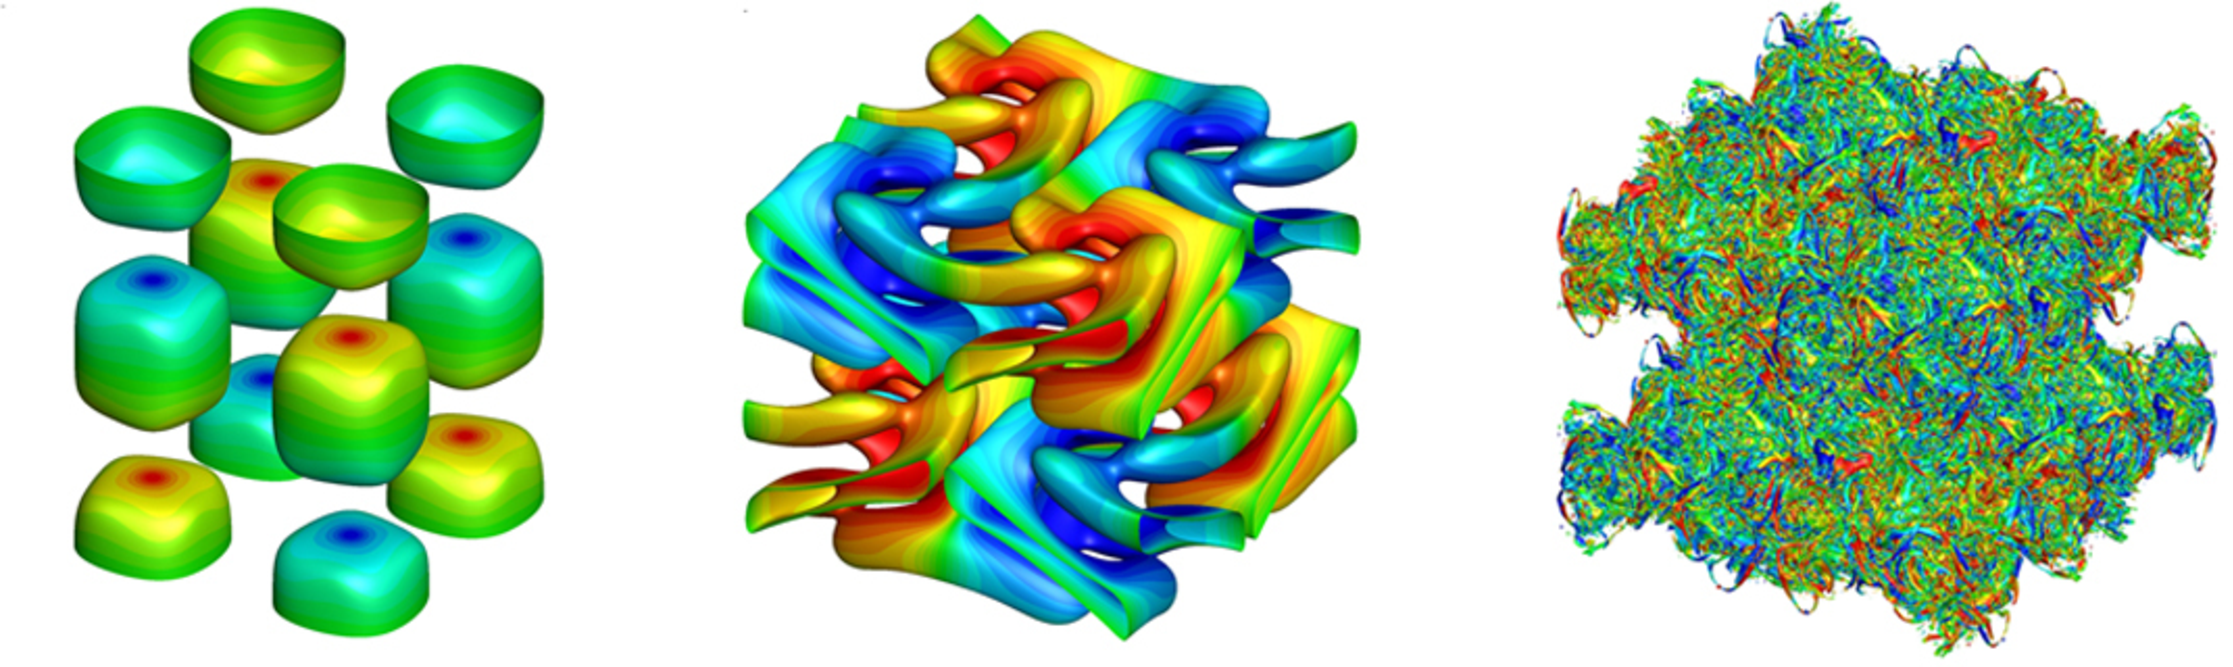
\includegraphics[width=1\textwidth]{figs/gassner_turb_01.pdf}
\caption*{Under-resolved solutions: turbulence (inviscid Taylor-Green vortex).}}
\only<2>{
\vspace{-.5em}
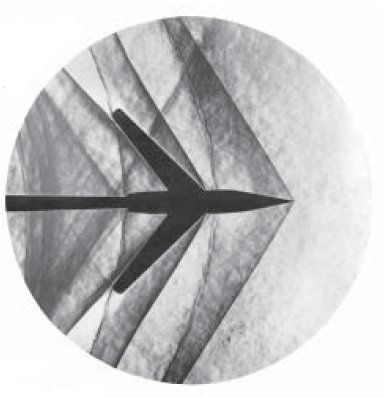
\includegraphics[width=.35\textwidth]{figs/shadowgraph.jpg}
\hspace{1em}
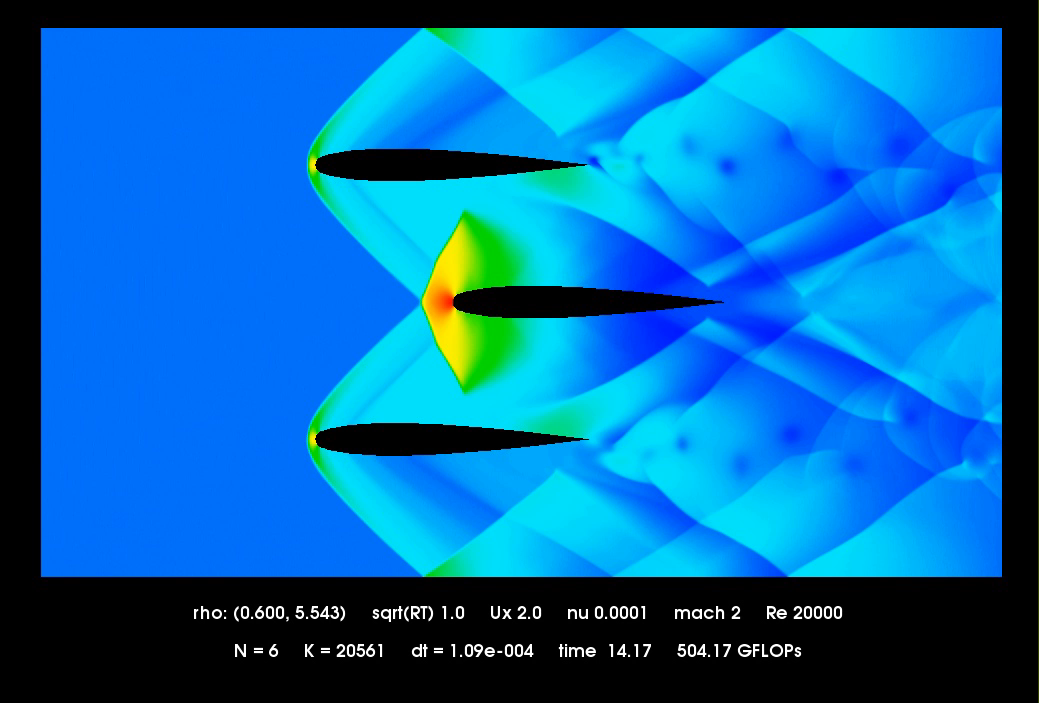
\includegraphics[width=.5\textwidth]{figs/trifoil.png}
\caption*{Under-resolved solutions: shock waves.}
}
\only<3>{
\vspace{1em}
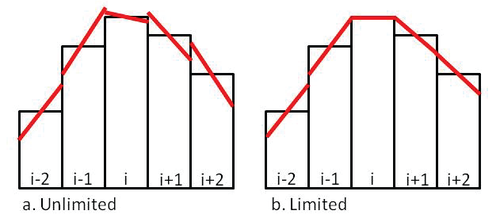
\includegraphics[width=.675\textwidth]{figs/slopeLimit.png}
\caption*{Slope limiting for a finite volume method.}
}
\only<4->{
\vspace{-1em}
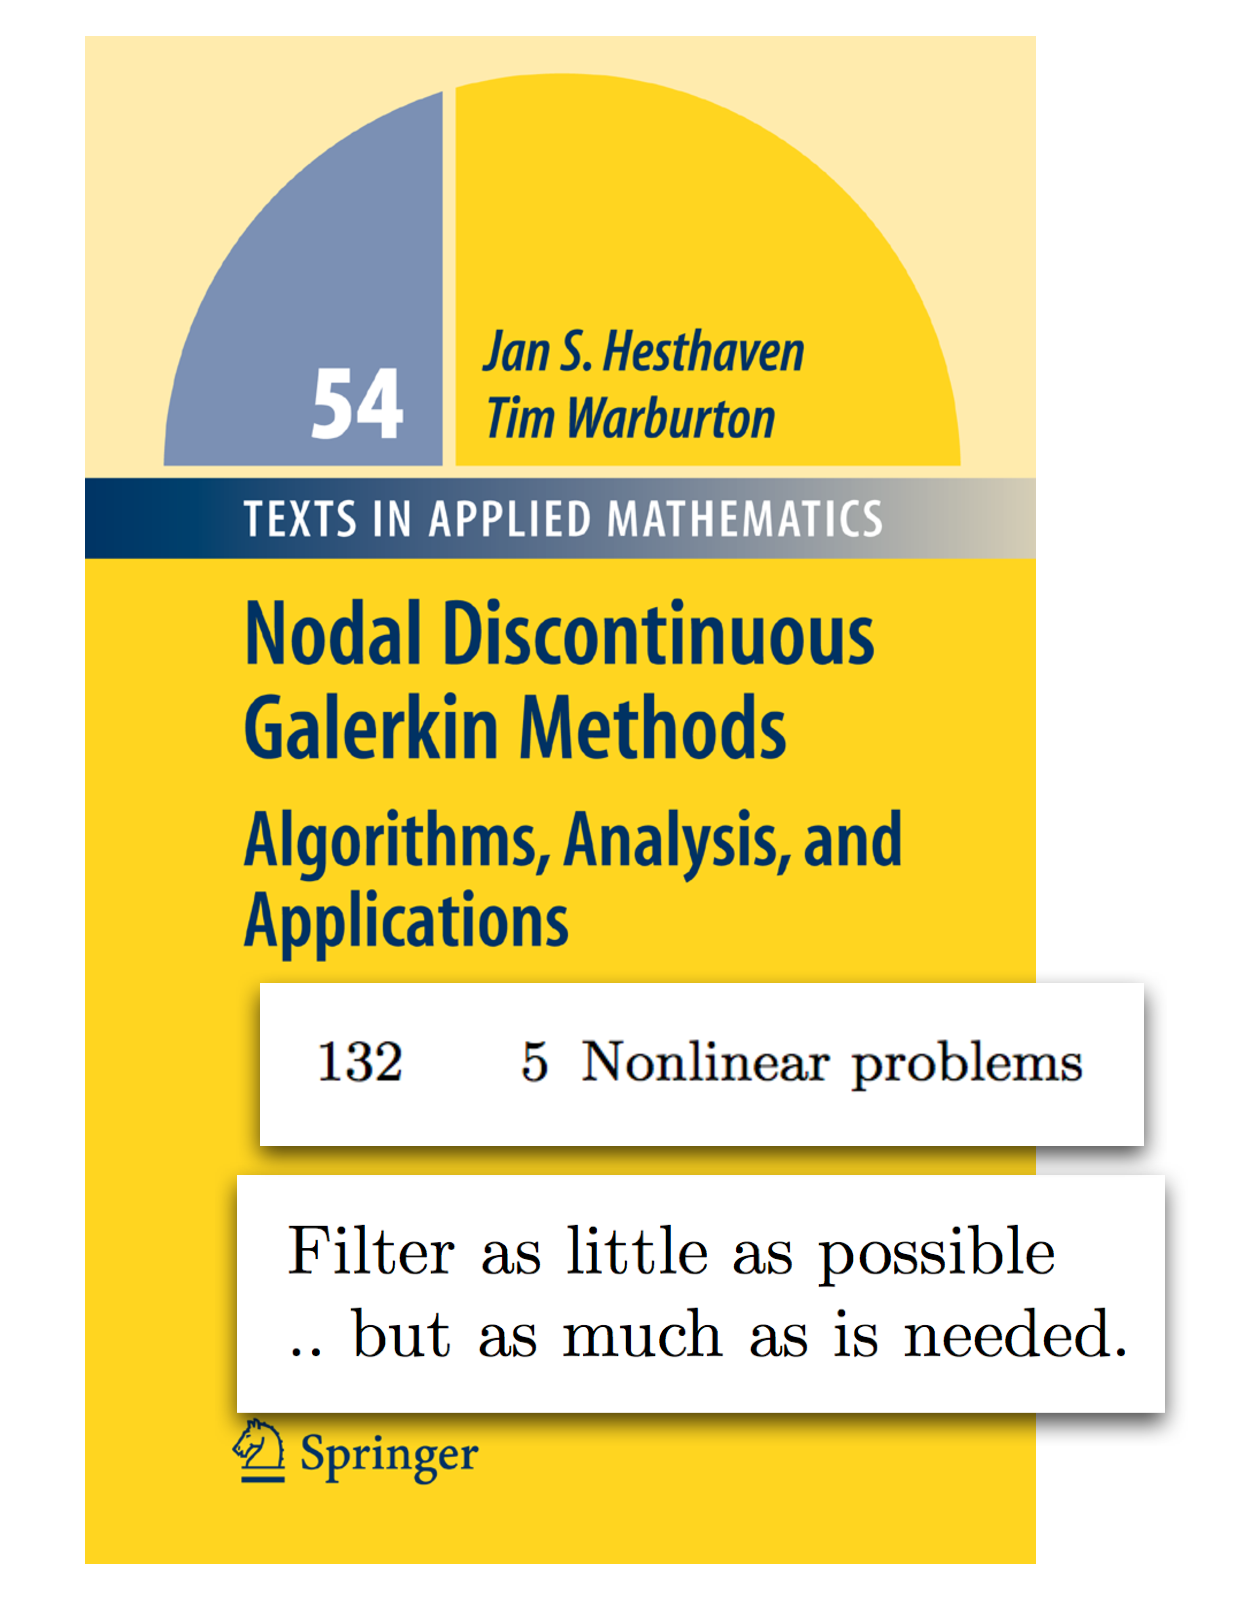
\includegraphics[width=.38\textwidth]{figs/ndgFilter.pdf}
\hspace{1em}
\visible<5>{\raisebox{2.5em}{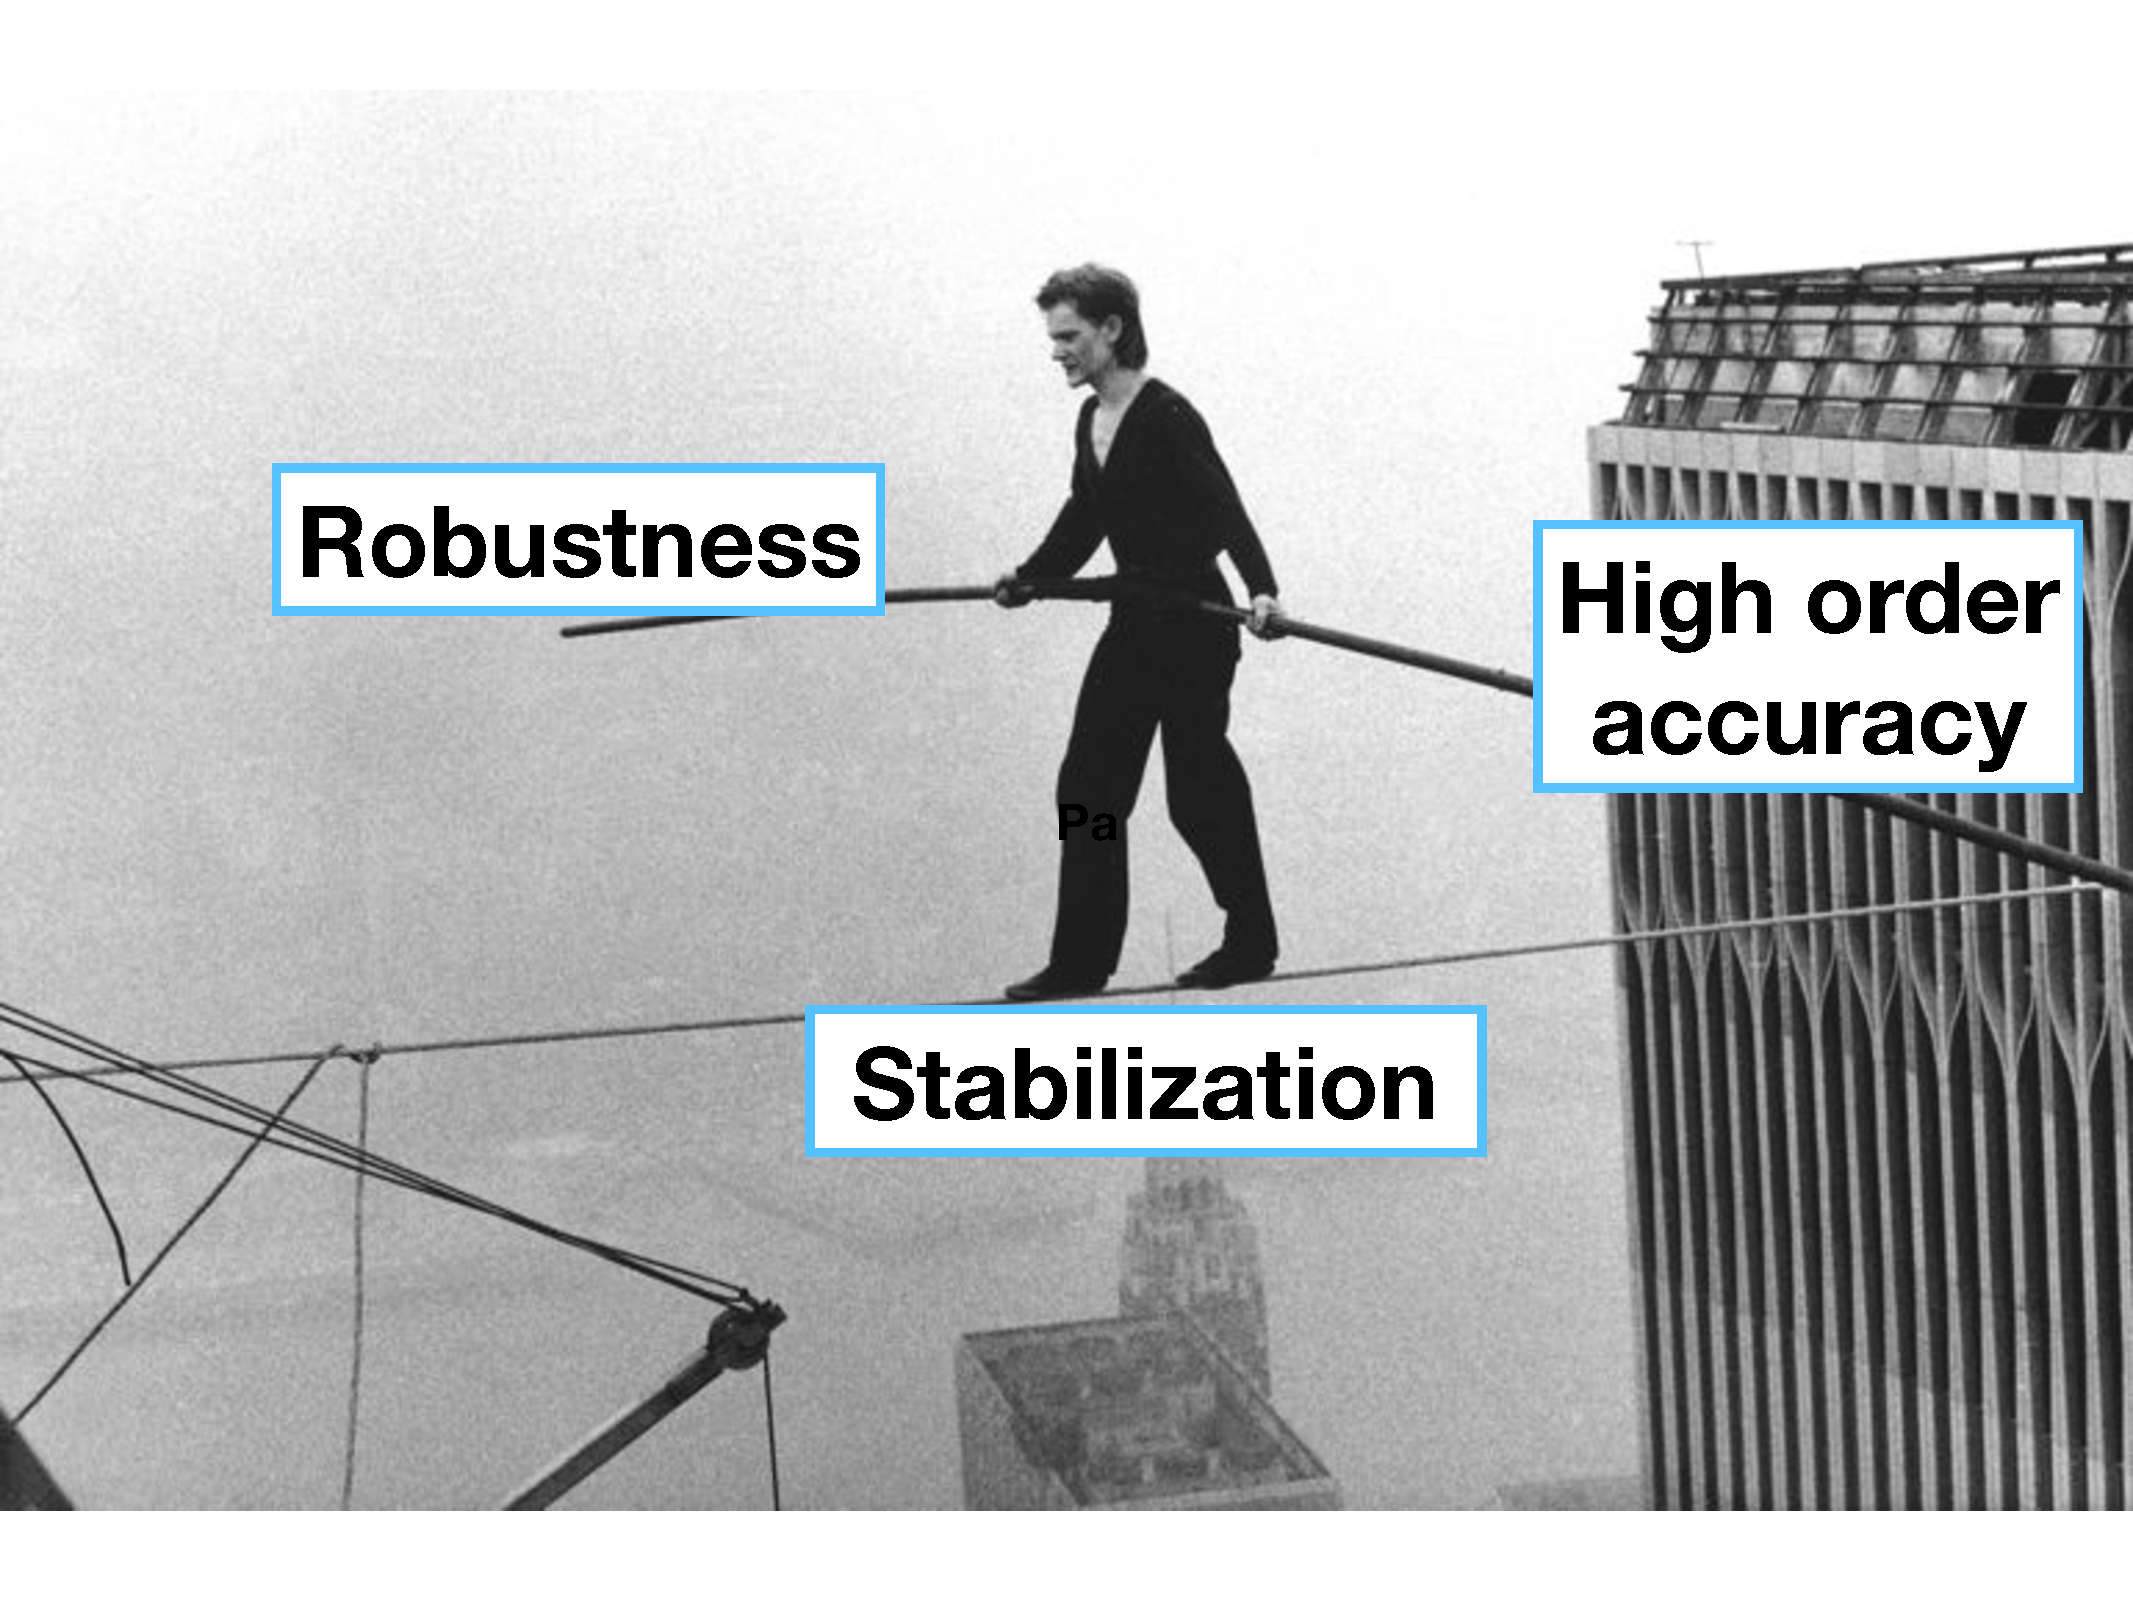
\includegraphics[width=.49\textwidth]{figs/balancing.pdf}}}
%\visible<5>{
\includegraphics[width=.475\textwidth]{figs/ductTape.png}}
}
\end{figure}
\end{overlayarea}
\let\thefootnote\relax\footnotetext{\tiny Figures courtesy of \href{http://www.gauss-centre.eu/gauss-centre/EN/Projects/CSE/2014/gassner_turbulence.html?nn=1345710}{Gregor Gassner}, T.\ Warburton, \href{http://cirpwiki.info/wiki/CMS-Flow_Numerical_Methods}{Coastal Inlets Research Program (CIRP)}.}
}

%% =================================================

%\section{Entropy stable formulations} 
%

\section{Summation by parts methods}

\frame[noframenumbering]{
\frametitle{Talk outline}
\tableofcontents[currentsection]
}

\frame{
\frametitle{Summation-by-parts (SBP) finite differences}
\setcounter{subfigure}{0}
\begin{itemize}
\item Finite differences satisfying matrix form of integration by parts.  
\item Related to nodal ``collocation'' DG and \textcolor{red}{under-integrated} quadrature, not necessarily associated with \textcolor{red}{basis or approximation space}. 
\end{itemize}
\vspace{-1em}
\begin{figure}
\centering
%\begingroup
%\captionsetup[subfloat]{width=.475\textwidth}
\subfloat[1D matrix ($N=2$, equispaced pts)]{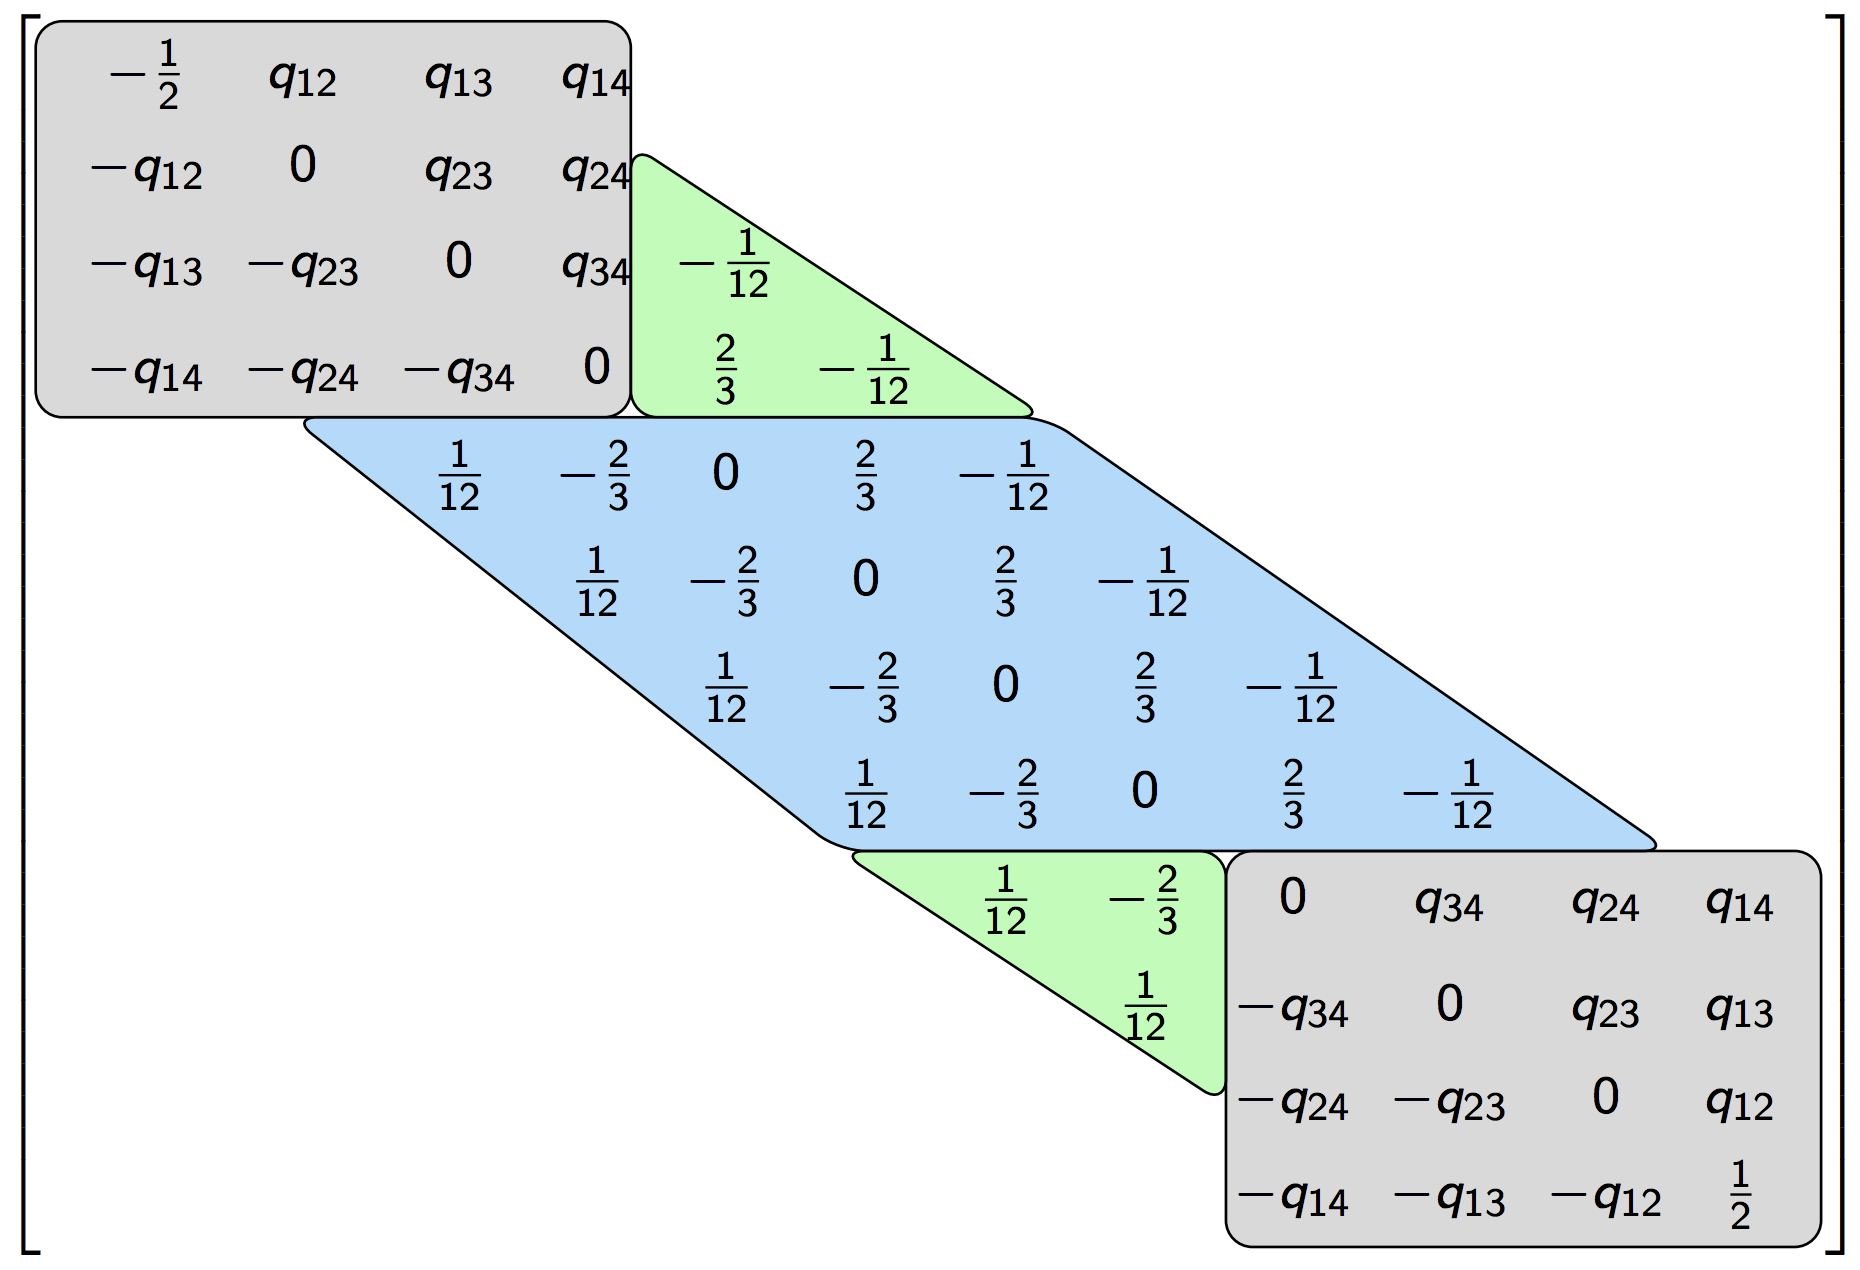
\includegraphics[width=.45\textwidth]{figs/sbp_dcdr.png}}
\hspace{1em}
\subfloat[2D SBP ($N=7$, GLL nodes)]{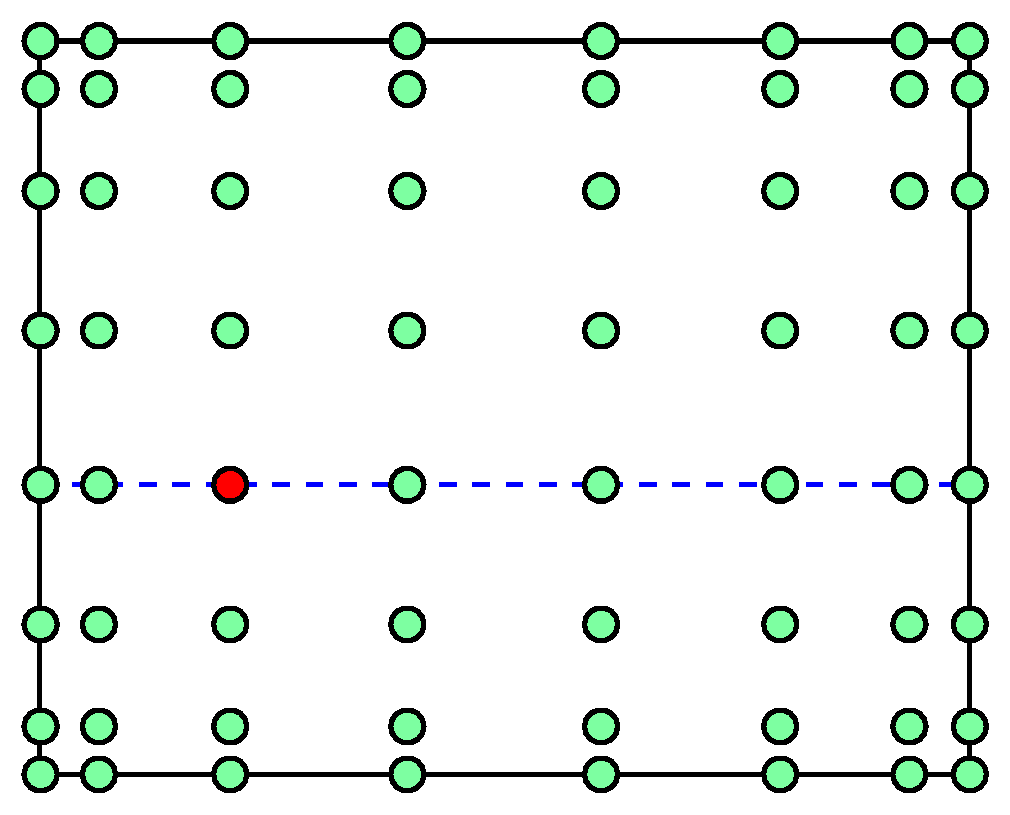
\includegraphics[width=.39\textwidth]{figs/SEM_stencil_1.pdf}}
%\subfloat[Diag-norm SBP nodes ($N=4$, 22 pts)]{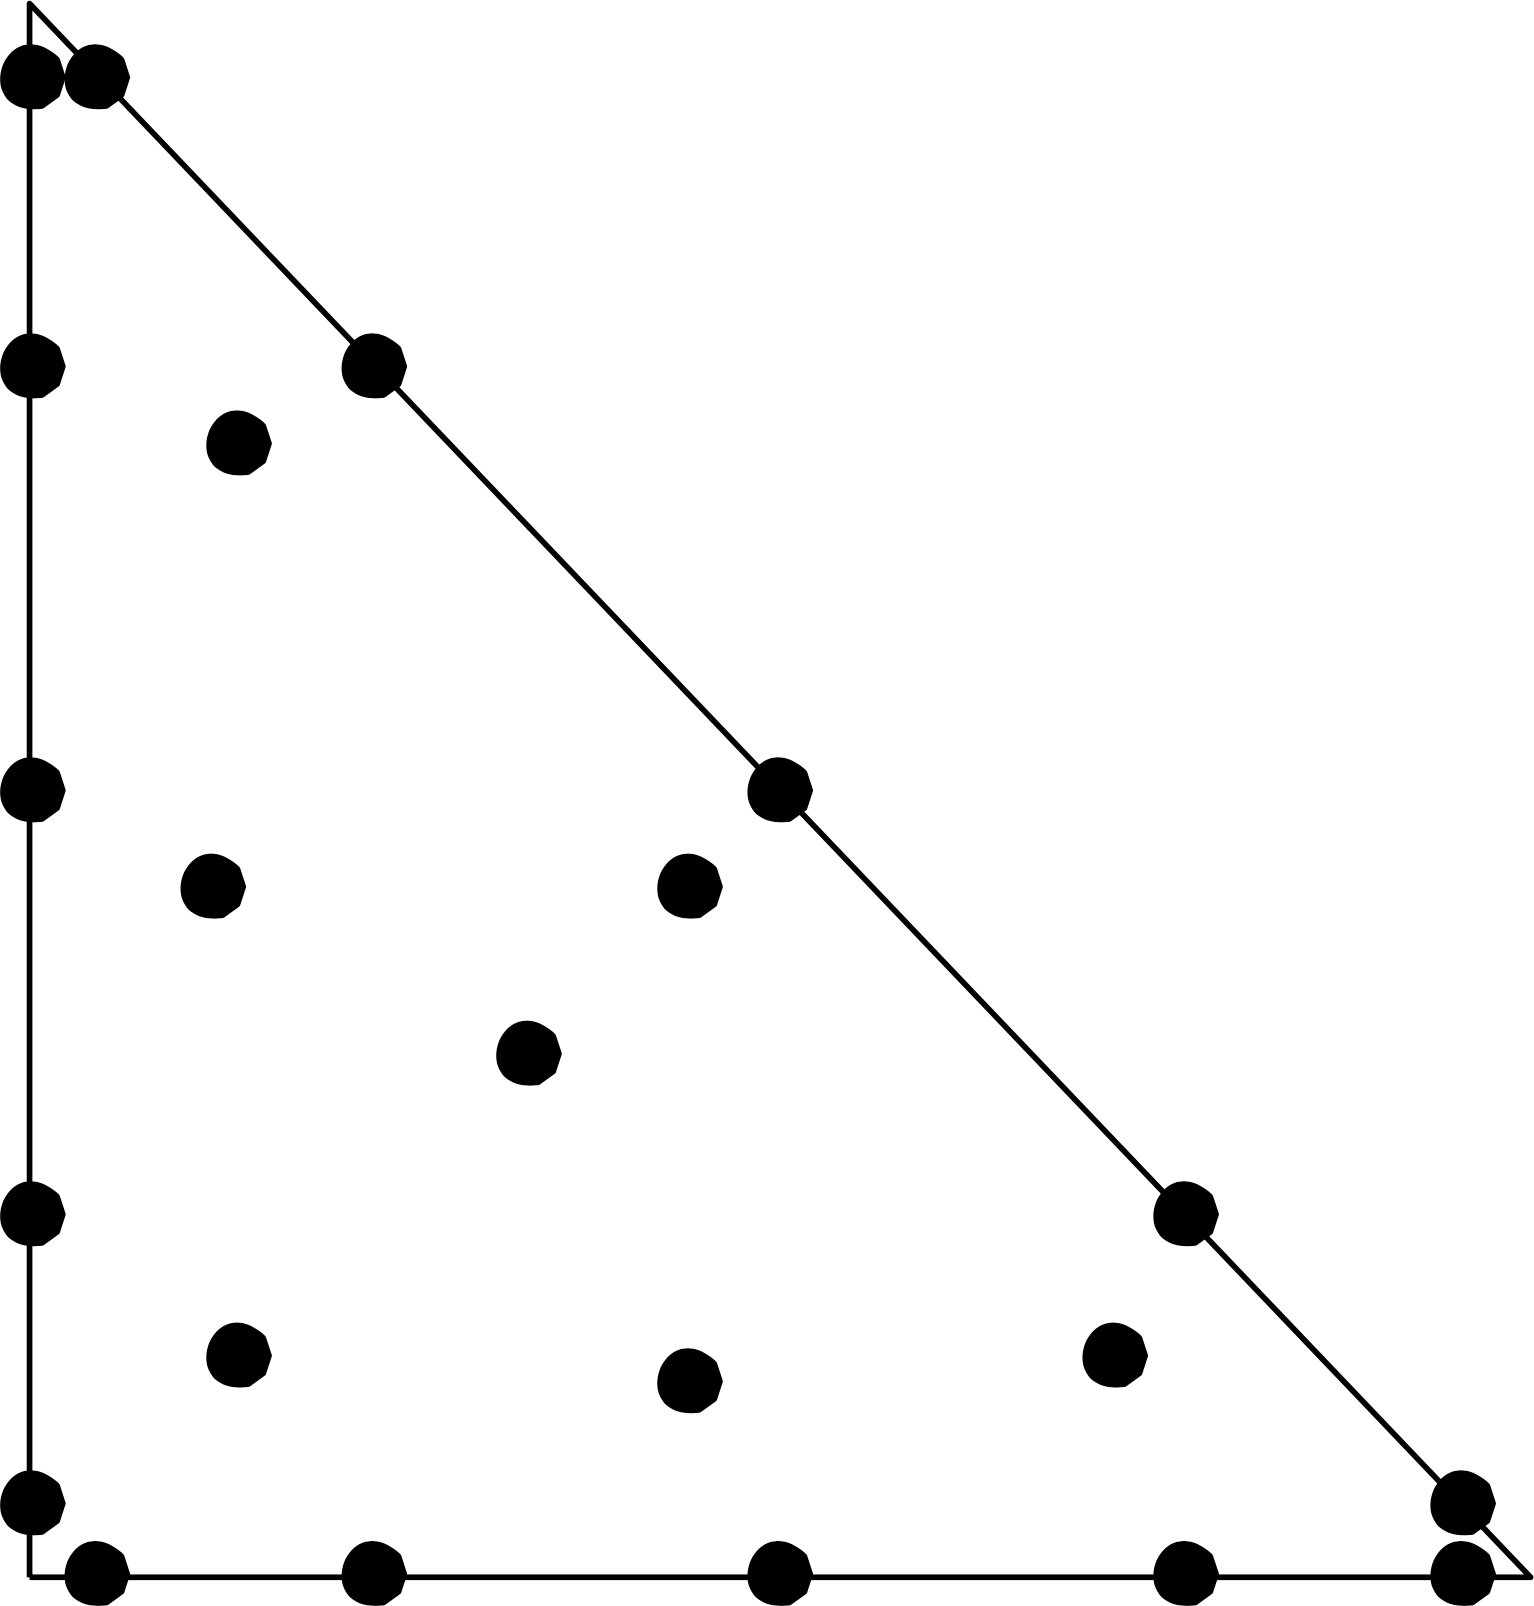
\includegraphics[height=.33\textheight]{figs/chenShuNodes.png}}
%\endgroup
%\caption{Dif.}
\end{figure}

\let\thefootnote\relax\footnotetext{\tiny Figure courtesy of David C.\ Del Rey Fernandez.}
\let\thefootnote\relax\footnotetext{\tiny Fisher and Carpenter (2013). \textit{High-order ES finite difference schemes for nonlinear conservation laws: Finite domains.} }
\let\thefootnote\relax\footnotetext{\tiny Gassner, Winters, and Kopriva (2016). \textit{Split form nodal DG schemes with SBP property for the comp.\ Euler equations.}}
%\let\thefootnote\relax\footnotetext{\tiny Chen and Shu (2017). \textit{ES high order DG methods with suitable quadrature rules for hyperbolic conservation laws.}}
%\let\thefootnote\relax\footnotetext{\tiny Crean, Hicken, et al.\ (2018). \textit{Entropy-stable SBP discretization of the Euler equations on general curved elements.}}
}


%
%\begin{itemize}
%\item
%\begin{align*}
%&\LRp{\bm{I}_n\otimes \bm{M}}\pd{\bm{u}}{t} + \LRp{2\LRp{\bm{I}_n\otimes \bm{M}\bm{D}}\circ \bm{F}_S}\bm{1} = 0,& &\text{(Semi-discrete form)}&\\
%&\Longrightarrow \bm{1}^T\LRp{\bm{M}\pd{S}{t} + \bm{B}\LRp{\bm{v}^T\bm{f} - \bm{\psi}}} = 0,& &\text{(Entropy conservation)}&
%\end{align*}
%\item Relies on diagonal mass matrix
%\[
%\bm{M} = {\rm diag}(\bm{w}),
%\qquad
%\begin{array}{c}
%\bm{Q} = \bm{M}\bm{D}\\
%\\
%\bm{Q}  = \bm{B} - \bm{S}^T
%\end{array}, 
%\qquad 
%\bm{B} = \left(\begin{array}{cccc}-1\\&0&&\\ &&\ddots& \\ & & & 1\end{array}\right).
%\]
%\begin{overlayarea}{\textwidth}{.275\textheight}
%\only<1>{
%\[
%\underbrace{\bm{M}\pd{\bm{u}}{t} + \LRp{2\bm{Q}\circ \bm{F}_S}\bm{1} = 0}_{\text{Semi-discrete form}}
%\]
%}
%\only<2>{
%\[
%\note{\underbrace{\bm{v}^T}_{\text{Test w/entropy vars}}}\LRp{\bm{M}\pd{\bm{u}}{t} + \LRp{2\bm{S} \circ \bm{F}_S}\bm{1}} = 0.
%\]
%}
%\only<3>{
%\[
%\note{\underbrace{\bm{1}^T\bm{M}\pd{S}{t}}_{
%\substack{\bm{v}^T\bm{M}\pd{\bm{u}}{t} = \bm{1}^T\bm{M}\pd{Q}{\bm{u}}^T\pd{\bm{u}}{t}\\ 
%\text{Diag }\bm{M}}
%}} + \bm{v}^T\LRp{2\bm{Q}\circ \bm{F}_S}\bm{1} = 0.
%\]
%}
%\only<4>{
%\[
%\bm{1}^T\bm{M}\pd{S}{t} + \bm{v}^T \bigg(\note{\underbrace{\LRp{\bm{B} + \bm{Q} - \bm{Q}^T}}_{\text{SBP}}} \circ \bm{F}_S\bigg)\bm{1} = 0
%\]
%}
%\only<5>{
%\[
%\bm{1}^T\bm{M}\pd{S}{t} + \note{\bm{v}^T\LRp{\bm{B} \circ \bm{F}_S}\bm{1} + \bm{v}^T\LRp{\LRp{\bm{Q} - \bm{Q}^T}\circ \bm{F}_S}\bm{1}} = 0
%\]
%}
%\only<6>{
%\[
%\bm{1}^T\bm{M}\pd{S}{t} + \note{\underbrace{\bm{1}^T\bm{B}\bm{v}^T\bm{f}}_{
%\substack{\bm{v}^T \LRp{\bm{B} \circ \bm{F}_S}\bm{1}\\ \text{Consistent }\bm{F}_S, \text{ diag }\bm{B}}
%}} + \bm{v}^T\LRp{\LRp{\bm{S} - \bm{S}^T}\circ \bm{F}_S}\bm{1} = 0. %\qquad \text{(Diag $\bm{B}$, $\bm{F}_S(\bm{u},\bm{u}) = \bm{f}(\bm{u})$)}
%\]
%}
%\only<7>{
%\[
%\bm{1}^T\bm{M}\pd{\bm{S}}{t} + \bm{1}^T\bm{B}\LRp{\bm{v}^T\bm{f} - \bm{\psi}} = 0.
%\]
%%\begin{center}
%$\Longrightarrow$ Discrete statement of entropy conservation!
%%\end{center}
%}
%\end{overlayarea}
%\end{itemize}
%}

\frame{
\frametitle{Quadrature-based matrices for polynomial bases}

\begin{itemize}
\item Volume and surface quadratures $(\bm{x}^q_i,\bm{w}^q_i)$, $(\bm{x}^f_i, \bm{w}^f_i)$, exact for degree $2N$ polynomials.  Define diagonal quadrature weight matrices
\[
\bm{W} = {\rm diag}\LRp{\bm{w}^q}, \qquad \bm{W}_f = {\rm diag}\LRp{\bm{w}^f}.
\]
\item Assume some polynomial basis $\phi_1,\ldots,\phi_{N_p}$.  Define differentiation matrix $\bm{D}^i$, interpolation matrices $\bm{V}_q, \bm{V}_f$
\[
\LRp{\bm{V}_q}_{ij} = \phi_j(\bm{x}^q_i), \qquad \LRp{\bm{V}_f}_{ij} = \phi_j(\bm{x}^f_i).
\]
\item Introduce quadrature-based $L^2$ \note{projection} and \note{lifting} matrices
\[
\bm{P}_q = \bm{M}^{-1}\bm{V}_q^T\bm{W}, \qquad \bm{L}_f = \bm{M}^{-1}\bm{V}_f^T\bm{W}_f.  
\]
\end{itemize}
}

\frame{
\frametitle{Quadrature-based differentiation matrices}

\begin{itemize}
\item Matrix $\bm{D}^i_q$: evaluates derivative of $L^2$ projection at points $\bm{x}^q$.
\[
\bm{D}^i_q = \bm{V}_q\bm{D}^i\bm{P}_q.  
\]
\item Summation-by-parts involving $L^2$ projection:
\[
\bm{W}\bm{D}^i_q + \LRp{\bm{W}\bm{D}^i_q }^T = \LRp{\bm{V}_f\bm{P}_q}^T\bm{W}_f{\rm diag}\LRp{\bm{n}_i}\bm{V}_f\bm{P}_q.
\]
\item Equivalent to integration-by-parts + quadrature: for $u, v \in L^2\LRp{\hat{D}}$ 
\[
\int_{\hat{D}} \pd{P_N u}{x_i}v + \int_{\hat{D}} u\pd{P_N v}{x_i} = \int_{\partial \hat{D}} \LRp{P_N u}\LRp{P_N v} \hat{n}_i
\]
\item $\bm{D}^i_q$ leads to generalized SBP methods; complicated \note{interface terms}.  
\end{itemize}

}

\frame{
\frametitle{A ``decoupled'' block SBP operator}
\begin{itemize}
\item Idea: incorporate \note{boundary traces} into approximation of derivative.
\vspace{.5em}
\item On an element $D^k$ with unit normal vector $\bm{n}$: approximate derivative w.r.t.\ the $i$th coordinate.
\begin{align*}
\bm{D}^i_N  &= \LRs{
\begin{array}{cc}
\bm{D}^i_q - \frac{1}{2}\bm{V}_q \bm{L}_f {\rm diag}({\bm{n}}_i) \bm{V}_f\bm{P}_q &  \frac{1}{2}\bm{V}_q\bm{L}_f{\rm diag}({\bm{n}}_i)\\
-\frac{1}{2}{\rm diag}({\bm{n}}_i)\bm{V}_f\bm{P}_q & \frac{1}{2}{\rm diag}({\bm{n}}_i)
\end{array}},
\label{eq:DN}
\end{align*}
\item $\bm{D}^i_N$ satisfies a summation-by-parts (SBP) property
\begin{gather*}
\bm{Q}^i_N = \LRs{\begin{array}{cc}
\bm{W} & \\
& \bm{W}_f
\end{array}}
\bm{D}^i_N, \qquad \bm{B}_N = \LRs{\begin{array}{cc}
0 & \\
& \bm{W}_f\bm{n}_i
\end{array}},
\end{gather*}
\[
\boxed{\bm{Q}^i_N + \LRp{\bm{Q}^i_N}^T = \bm{B}_N} \sim \boxed{\int_{D^k} \pd{f}{x_i} g + f\pd{g}{x_i} = \int_{\partial D^k} fg\bm{n}_i}.
\]
\end{itemize}
}

\frame{
\frametitle{Differentiation using decoupled SBP operators}
\begin{itemize}
\item Note: $\bm{D}^i_N$ is \note{not} a differentiation matrix on its own.
\vspace{.5em}
\item $\bm{D}^i_N$ produces a high order approximation of $f\pd{g}{x}$ at $\bm{x} = [\bm{x}^q, \bm{x}^f]$.
\[
f\pd{g}{x} \approx \LRs{\begin{array}{cc}
\bm{P}_q & \bm{L}_f\end{array}} {\rm diag}\LRp{\bm{f}}\bm{D}_N \bm{g}, \qquad \bm{f}_i, \bm{g}_i = f(\bm{x}_i), g(\bm{x}_i).
\]
\item Equivalent to solving variational problem for $u(\bm{x}) \approx f\pd{g}{x}$
\[
\int_{D^k}u(\bm{x})v(\bm{x})  = \int_{D^k}{f\pd{P_Ng}{x}v} + \int_{\partial D^k}{(f-P_Nf)\frac{\LRp{gv + P_N(gv)}}{2}}.
\]
\item $\bm{D}^i_N \bm{1} = 0$ holds (necessary for discrete entropy conservation).
\end{itemize}
}

\frame{
\frametitle{Unifying multiple SBP formulations}
\setcounter{subfigure}{0}
\vspace{-.75em}
\begin{figure}
\centering
%\subfloat[SBP]{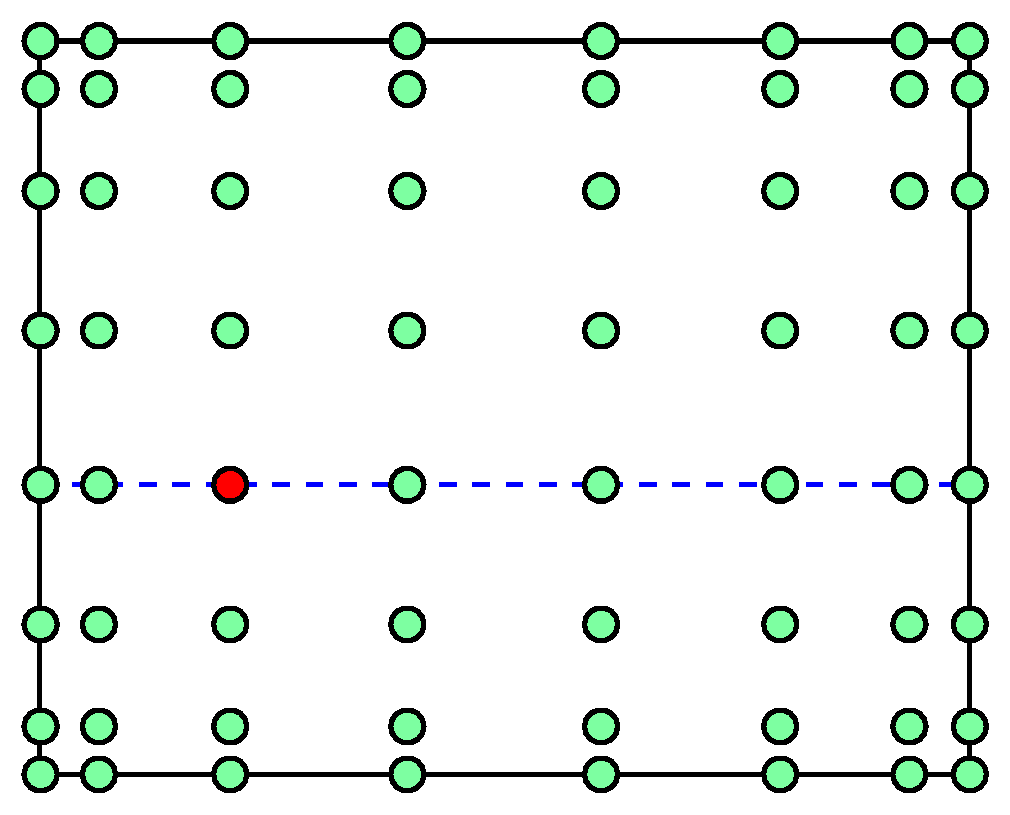
\includegraphics[height=.345\textheight]{figs/SEM_stencil_1.pdf}}
%\hspace{1em}
%\begingroup
%\captionsetup[subfloat]{width=.27\textwidth}
\subfloat[Generalized SBP]{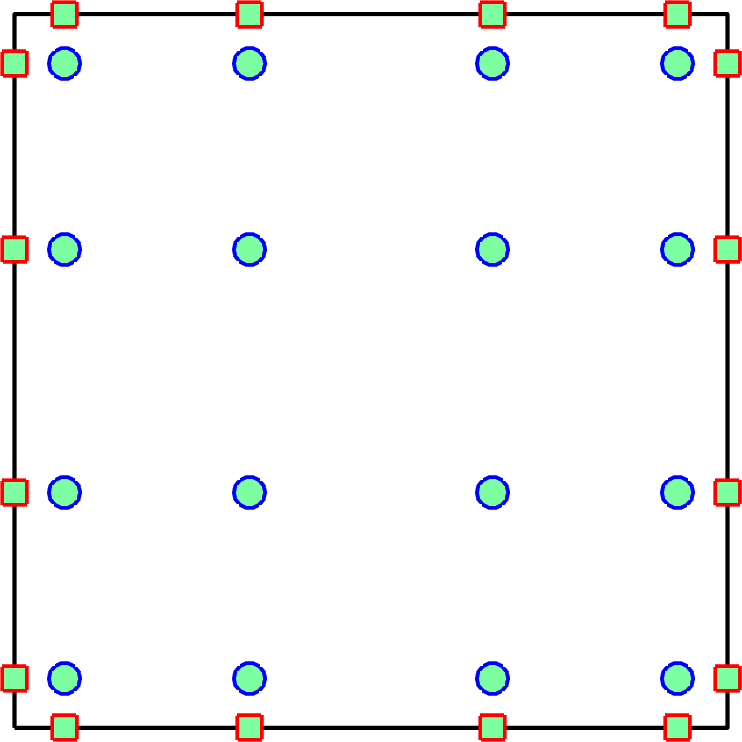
\includegraphics[height=.37\textheight]{figs/gsbp.png}}
\hspace{1em}
\subfloat[Staggered-grid SBP]{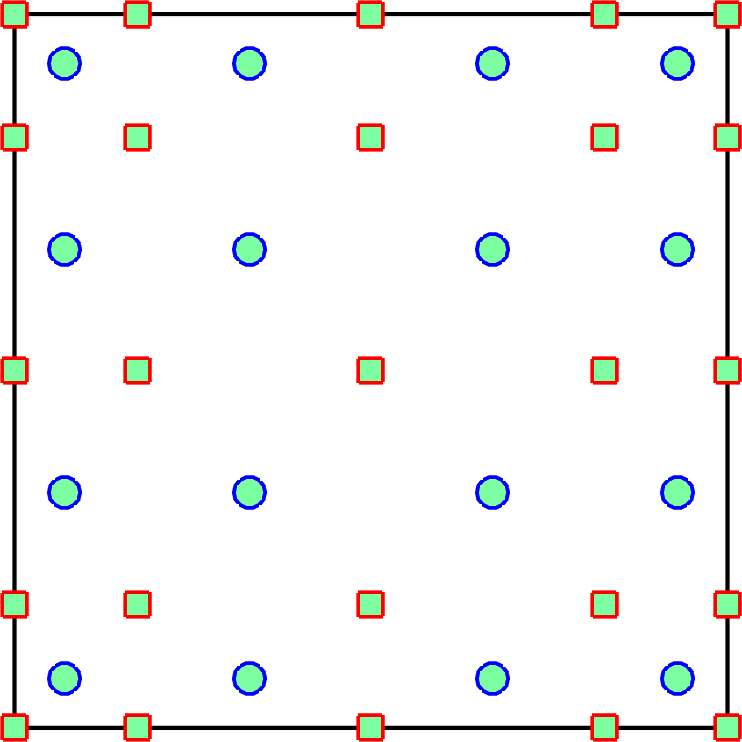
\includegraphics[height=.37\textheight]{figs/staggered.png}}
\hspace{.5em}
%\subfloat[Triangular SBP]{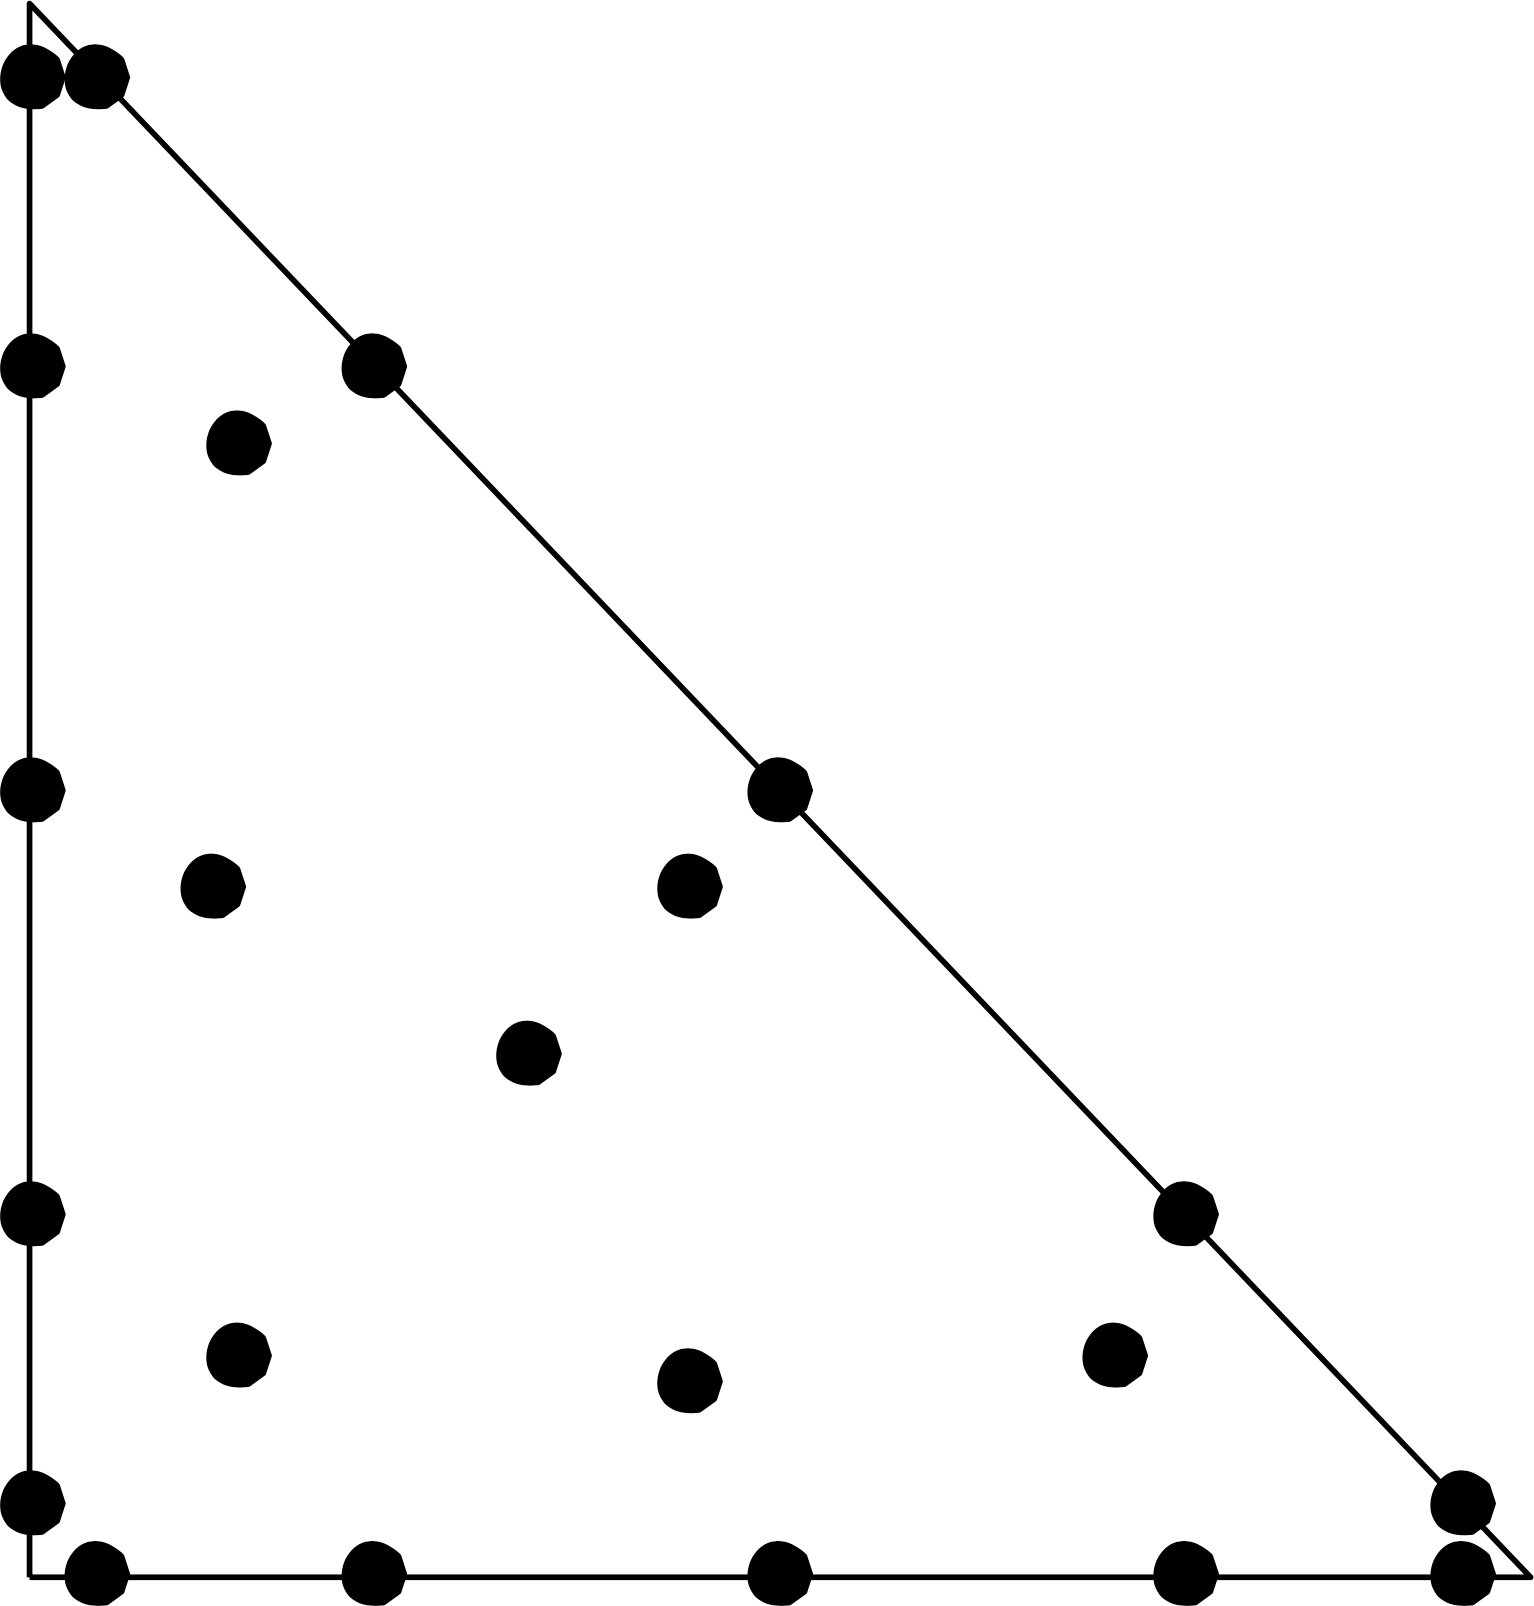
\includegraphics[height=.35\textheight]{figs/chenShuNodes.png}}
\subfloat[Triangular SBP]{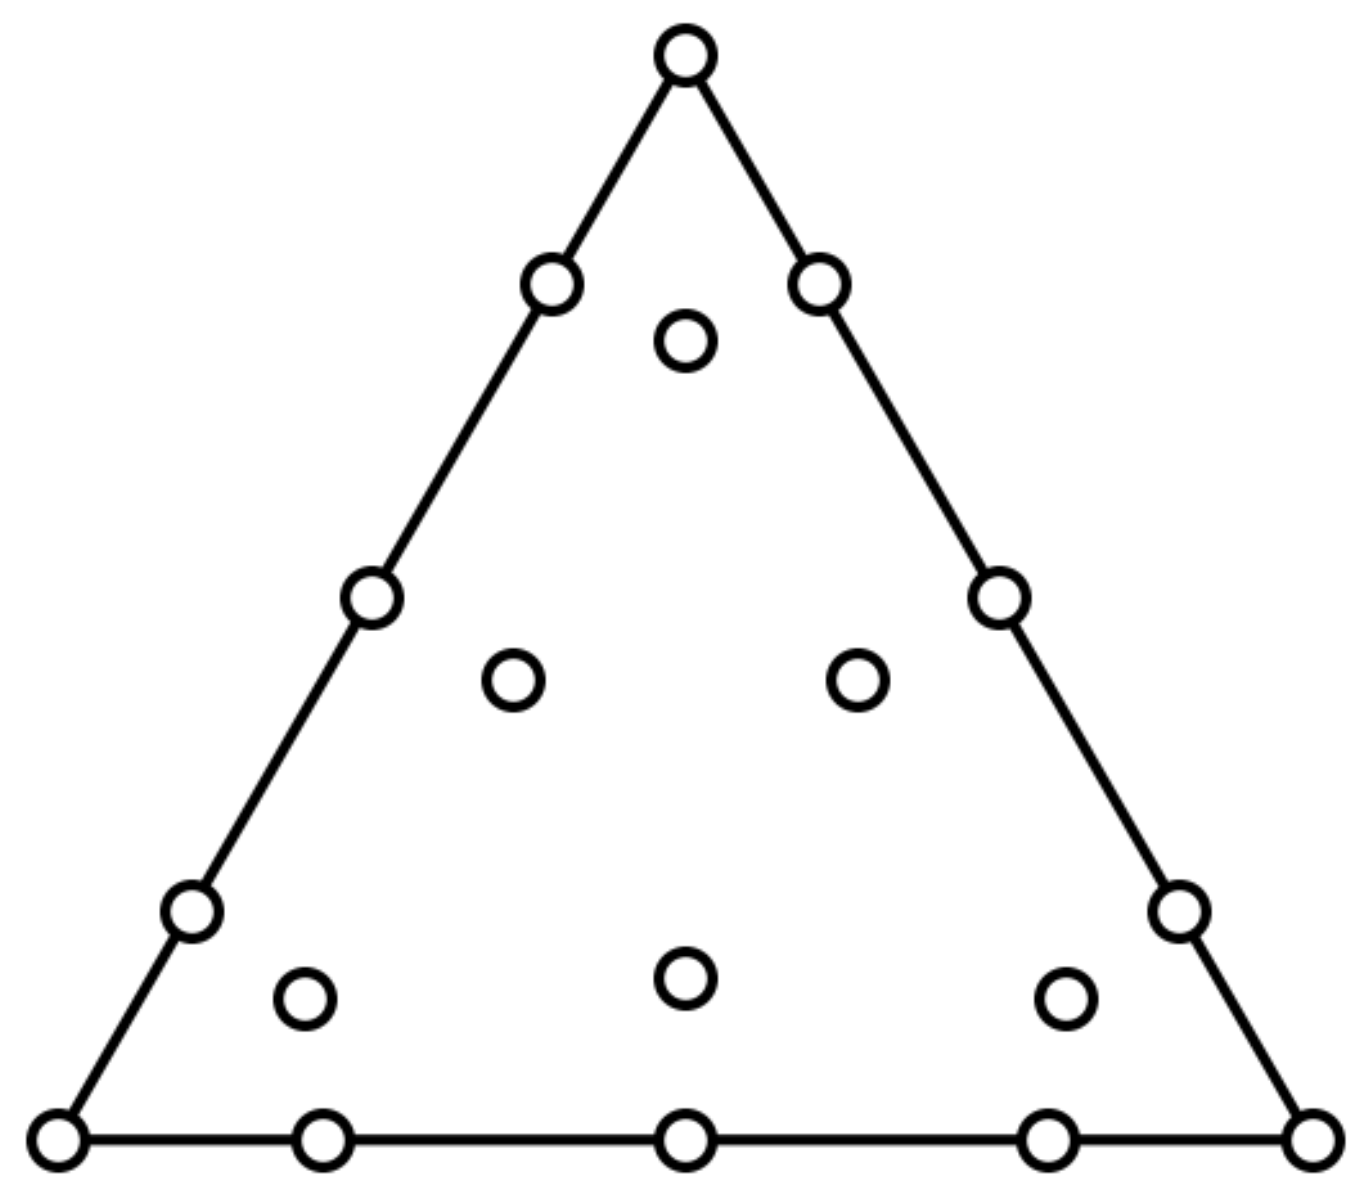
\includegraphics[height=.36\textheight]{figs/creanSBP.png}}
%\endgroup
\end{figure}
\begin{itemize}
\item Specific basis and quadratures recover existing stable discretizations (DG-SEM, Gauss-Legendre collocation, staggered grid, etc).  
\vspace{.1em}
\item Recovers existing (and new) interface coupling terms (SBP-SATs).  
\vspace{.1em}
\item Setting $\bm{P}_q = \bm{I}$ recovers non-basis SBP finite differences (simplices).  
\end{itemize}

\let\thefootnote\relax\footnotetext{\tiny Parsani et al.\  (2016). \emph{ES staggered grid disc.\ spectral collocation methods of any order for the comp.\ NS eqns.}}
%\let\thefootnote\relax\footnotetext{\tiny Hicken, Del Rey Fernandez, and Zingg (2016). \emph{Multidimensional summation-by-parts operators.}}
\let\thefootnote\relax\footnotetext{\tiny Crean, Hicken, et al.\ (2018). \textit{Entropy-stable SBP discretization of the Euler equations on general curved elements.}}
%\let\thefootnote\relax\footnotetext{\tiny Chen and Shu (2017). \textit{ES high order DG methods with suitable quadrature rules for hyperbolic conservation laws.}}
}


\section{Stable formulations and flux differencing}
\frame[noframenumbering]{
\frametitle{Talk outline}
\tableofcontents[currentsection]
}

\frame{
\frametitle{Burgers' equation: energy stable formulations}
\setcounter{subfigure}{0}
\begin{itemize}
\item \note{Split} form of Burgers' equation
\[
\pd{u}{t} + \frac{1}{3}\LRp{\pd{u^2}{x} + {u\pd{u}{x}}} = 0
\]
\item Stable DG method: let $u(x) = \sum_j \hat{\bm{u}}_j \phi(x)$.  Find $\hat{\bm{u}}$ such that 
\begin{align*}
&\bm{u} = \LRs{\begin{array}{c}
\bm{V}_q\\
\bm{V}_f
\end{array}} \hat{\bm{u}}, \qquad \bm{f}^* = \bm{f}^*(u^+,u) = \text{numerical flux} \\
&\td{\hat{\bm{u}}}{t} + \frac{1}{3}
\LRs{\begin{array}{cc}
\bm{P}_q & \bm{L}_f\end{array}}
\LRp{\bm{D}_N \LRp{\bm{u}^2} + {\rm diag}\LRp{\bm{u}} \bm{D}_N \bm{u}} + \bm{L}_f (\bm{f}^*) = 0.
\end{align*}
\item Energy estimate: multiply by $\hat{\bm{u}}^T\bm{M}$, use SBP, sum over $D^k$
\[
\sum_k \frac{1}{2}\td{}{t}\hat{\bm{u}}^T\bm{M}\hat{\bm{u}} = \sum_k \frac{1}{2} \pd{}{t}\nor{u}^2_{L^2\LRp{D^k}} \leq 0.
\]
\end{itemize}
}

\frame{
\frametitle{Burgers' equation: energy stable shock solution}
\setcounter{subfigure}{0}

\begin{figure}
\begin{overlayarea}{\textwidth}{.5\textheight}
%\begin{overprint}
\centering
\foreach \id in {1,2,3,4,5,6,7,8}{%
\only<\id>{
\subfloat[$\tau = 0$]{\includegraphics[width=.425\textwidth]{figs/burgersStableEC_\id.png}}\hspace{2em}%
\subfloat[$\tau = 1$]{\includegraphics[width=.425\textwidth]{figs/burgersStableLF_\id.png}}
}% \only
}% for
\only<9>{
\captionsetup[subfloat]{width=.45\textwidth, justification=centering}
\subfloat[Energy conservative ($\tau = 0$)]{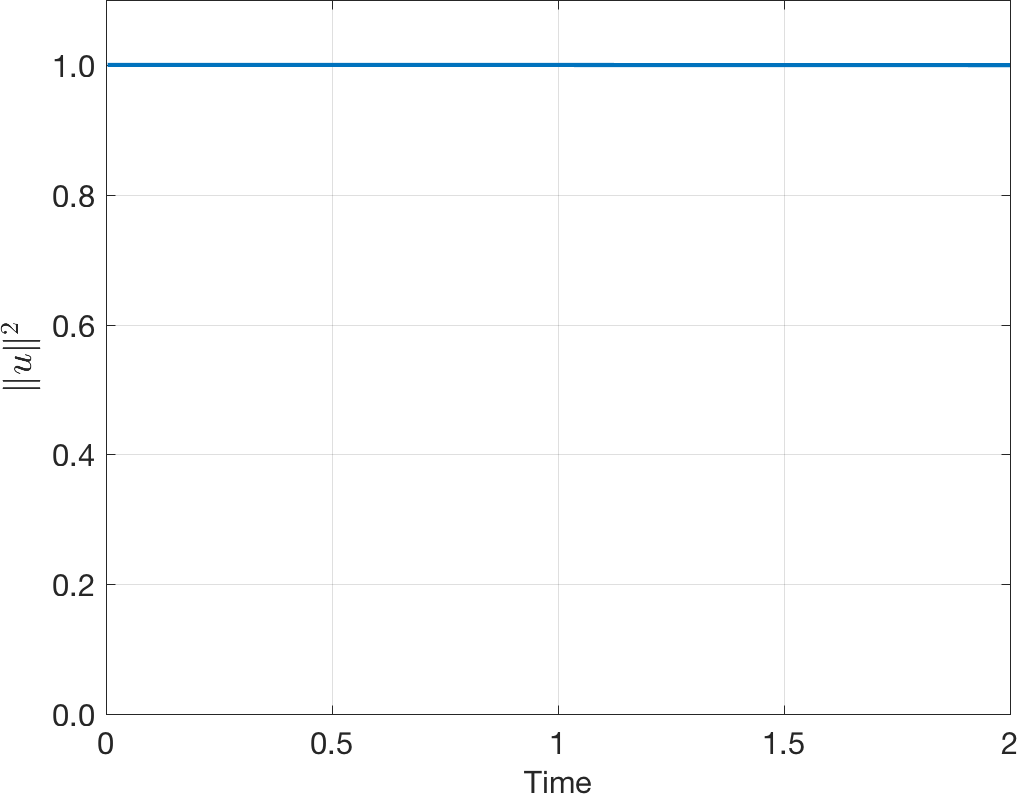
\includegraphics[width=.45\textwidth]{figs/burgersSplitEnergyEC.png}}\hspace{1em}%
\subfloat[Energy stable ($\tau = 1$)]{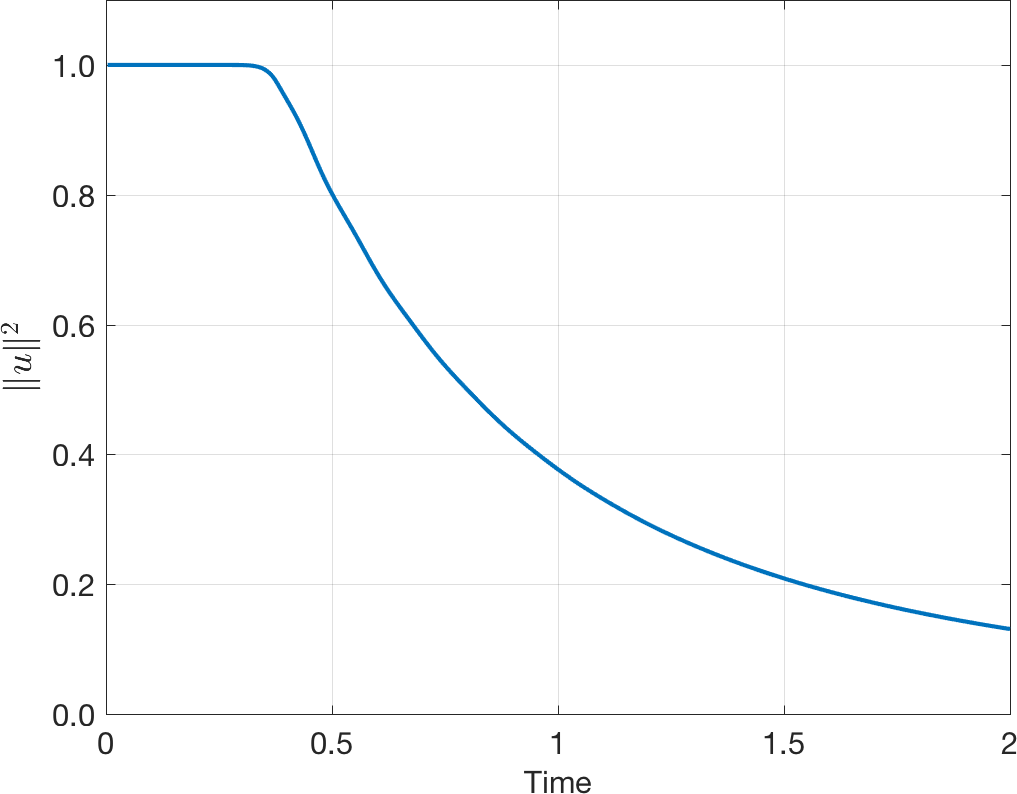
\includegraphics[width=.45\textwidth]{figs/burgersSplitEnergyLF.png}}
}
%\end{overprint}
\end{overlayarea}
\end{figure}
}


%% =================================================

%\frame{
%\frametitle{Entropy conservative summation-by-parts (SBP) methods}
%
%\begin{itemize}
%\item Pioneering work relies on \note{mass lumping, nodal collocation + SBP}.  	
%%\item Construction using \note{nodal collocation} at quadrature points.  
%\item Need at least $2N-1$ accurate volume and surface quadrature! 
%\item Difficult to generalize beyond polynomials (splines, pyramids, etc).  
%%\begin{align*}
%%&\LRp{\bm{I}_n\otimes \bm{M}}\pd{\bm{u}}{t} + \LRp{2\LRp{\bm{I}_n\otimes \bm{M}\bm{D}}\circ \bm{F}_S}\bm{1} = 0,& &\text{(Semi-discrete form)}&\\
%%&\Longrightarrow \bm{1}^T\LRp{\bm{M}\pd{S}{t} + \bm{B}\LRp{\bm{v}^T\bm{f} - \bm{\psi}}} = 0,& &\text{(Entropy conservation)}&
%%\end{align*}
%%\item Relies on diagonal norm SBP finite differences (e.g.\ DG-SEM).
%%\[
%%\bm{M} = {\rm diag}(\bm{w}),
%%\qquad
%%\begin{array}{c}
%%\bm{S} = \bm{M}\bm{D}\\
%%\\
%%\bm{S}  = \bm{B} - \bm{S}^T
%%\end{array}, 
%%\qquad 
%%\bm{B} = \left(\begin{array}{cccc}-1\\&0&&\\ &&\ddots& \\ & & & 1\end{array}\right).
%%\]
%%\begin{overlayarea}{\textwidth}{.275\textheight}
%%\only<1>{
%%\[
%%\underbrace{\bm{M}\pd{\bm{u}}{t} + \LRp{2\bm{S}\circ \bm{F}_S}\bm{1} = 0}_{\text{Semi-discrete form}}
%%\]
%%}
%%\only<2>{
%%\[
%%\note{\underbrace{\bm{v}^T}_{\text{Test w/entropy vars}}}\LRp{\bm{M}\pd{\bm{u}}{t} + \LRp{2\bm{S} \circ \bm{F}_S}\bm{1}} = 0.
%%\]
%%}
%%\only<3>{
%%\[
%%\note{\underbrace{\bm{1}^T\bm{M}\pd{S}{t}}_{
%%\substack{\bm{v}^T\bm{M}\pd{\bm{u}}{t} = \bm{1}^T\bm{M}\pd{S}{\bm{u}}^T\pd{\bm{u}}{t}\\ 
%%\text{Diag }\bm{M}}
%%}} + \bm{v}^T\LRp{2\bm{S}\circ \bm{F}_S}\bm{1} = 0.
%%\]
%%}
%%\only<4>{
%%\[
%%\bm{1}^T\bm{M}\pd{S}{t} + \bm{v}^T \bigg(\note{\underbrace{\LRp{\bm{B} + \bm{S} - \bm{S}^T}}_{\text{SBP}}} \circ \bm{F}_S\bigg)\bm{1} = 0
%%\]
%%}
%%\only<5>{
%%\[
%%\bm{1}^T\bm{M}\pd{S}{t} + \note{\bm{v}^T\LRp{\bm{B} \circ \bm{F}_S}\bm{1} + \bm{v}^T\LRp{\LRp{\bm{S} - \bm{S}^T}\circ \bm{F}_S}\bm{1}} = 0
%%\]
%%}
%%\only<6>{
%%\[
%%\bm{1}^T\bm{M}\pd{S}{t} + \note{\underbrace{\bm{1}^T\bm{B}\bm{v}^T\bm{f}}_{
%%\substack{\bm{v}^T \LRp{\bm{B} \circ \bm{F}_S}\bm{1}\\ \text{Consistent }\bm{F}_S, \text{ diag }\bm{B}}
%%}} + \bm{v}^T\LRp{\LRp{\bm{S} - \bm{S}^T}\circ \bm{F}_S}\bm{1} = 0. %\qquad \text{(Diag $\bm{B}$, $\bm{F}_S(\bm{u},\bm{u}) = \bm{f}(\bm{u})$)}
%%\]
%%}
%%\only<7>{
%%\[
%%\bm{1}^T\bm{M}\pd{\bm{S}}{t} + \bm{1}^T\bm{B}\LRp{\bm{v}^T\bm{f} - \bm{\psi}} = 0.
%%\]
%%%\begin{center}
%%$\Longrightarrow$ Discrete statement of entropy conservation!
%%%\end{center}
%%}
%%\end{overlayarea}
%\end{itemize}
%\vspace{-1em}
%\begin{figure}
%\centering
%\begingroup
%\captionsetup[subfloat]{width=.275\textwidth}
%\subfloat[Tensor product SBP nodes (GLL quadrature)]{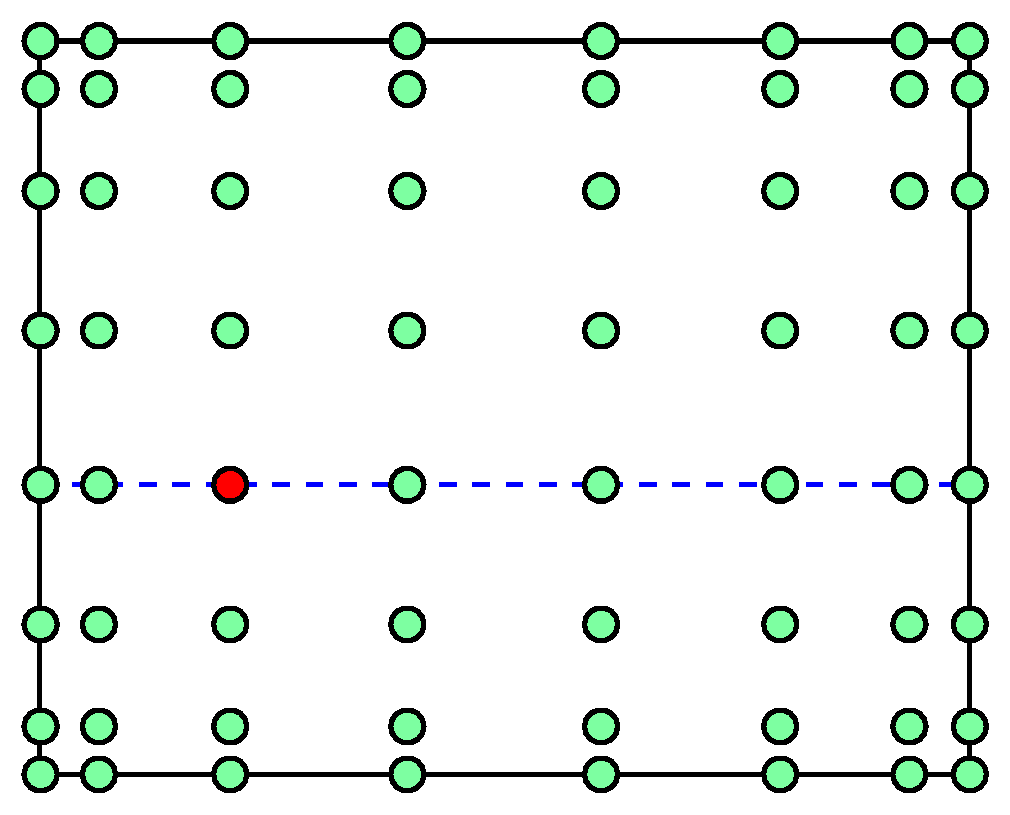
\includegraphics[width=.25\textwidth]{figs/SEM_stencil_1.pdf}}
%\hspace{2.5em}
%\subfloat[Diag-norm SBP nodes ($N=4$, 22 pts)]{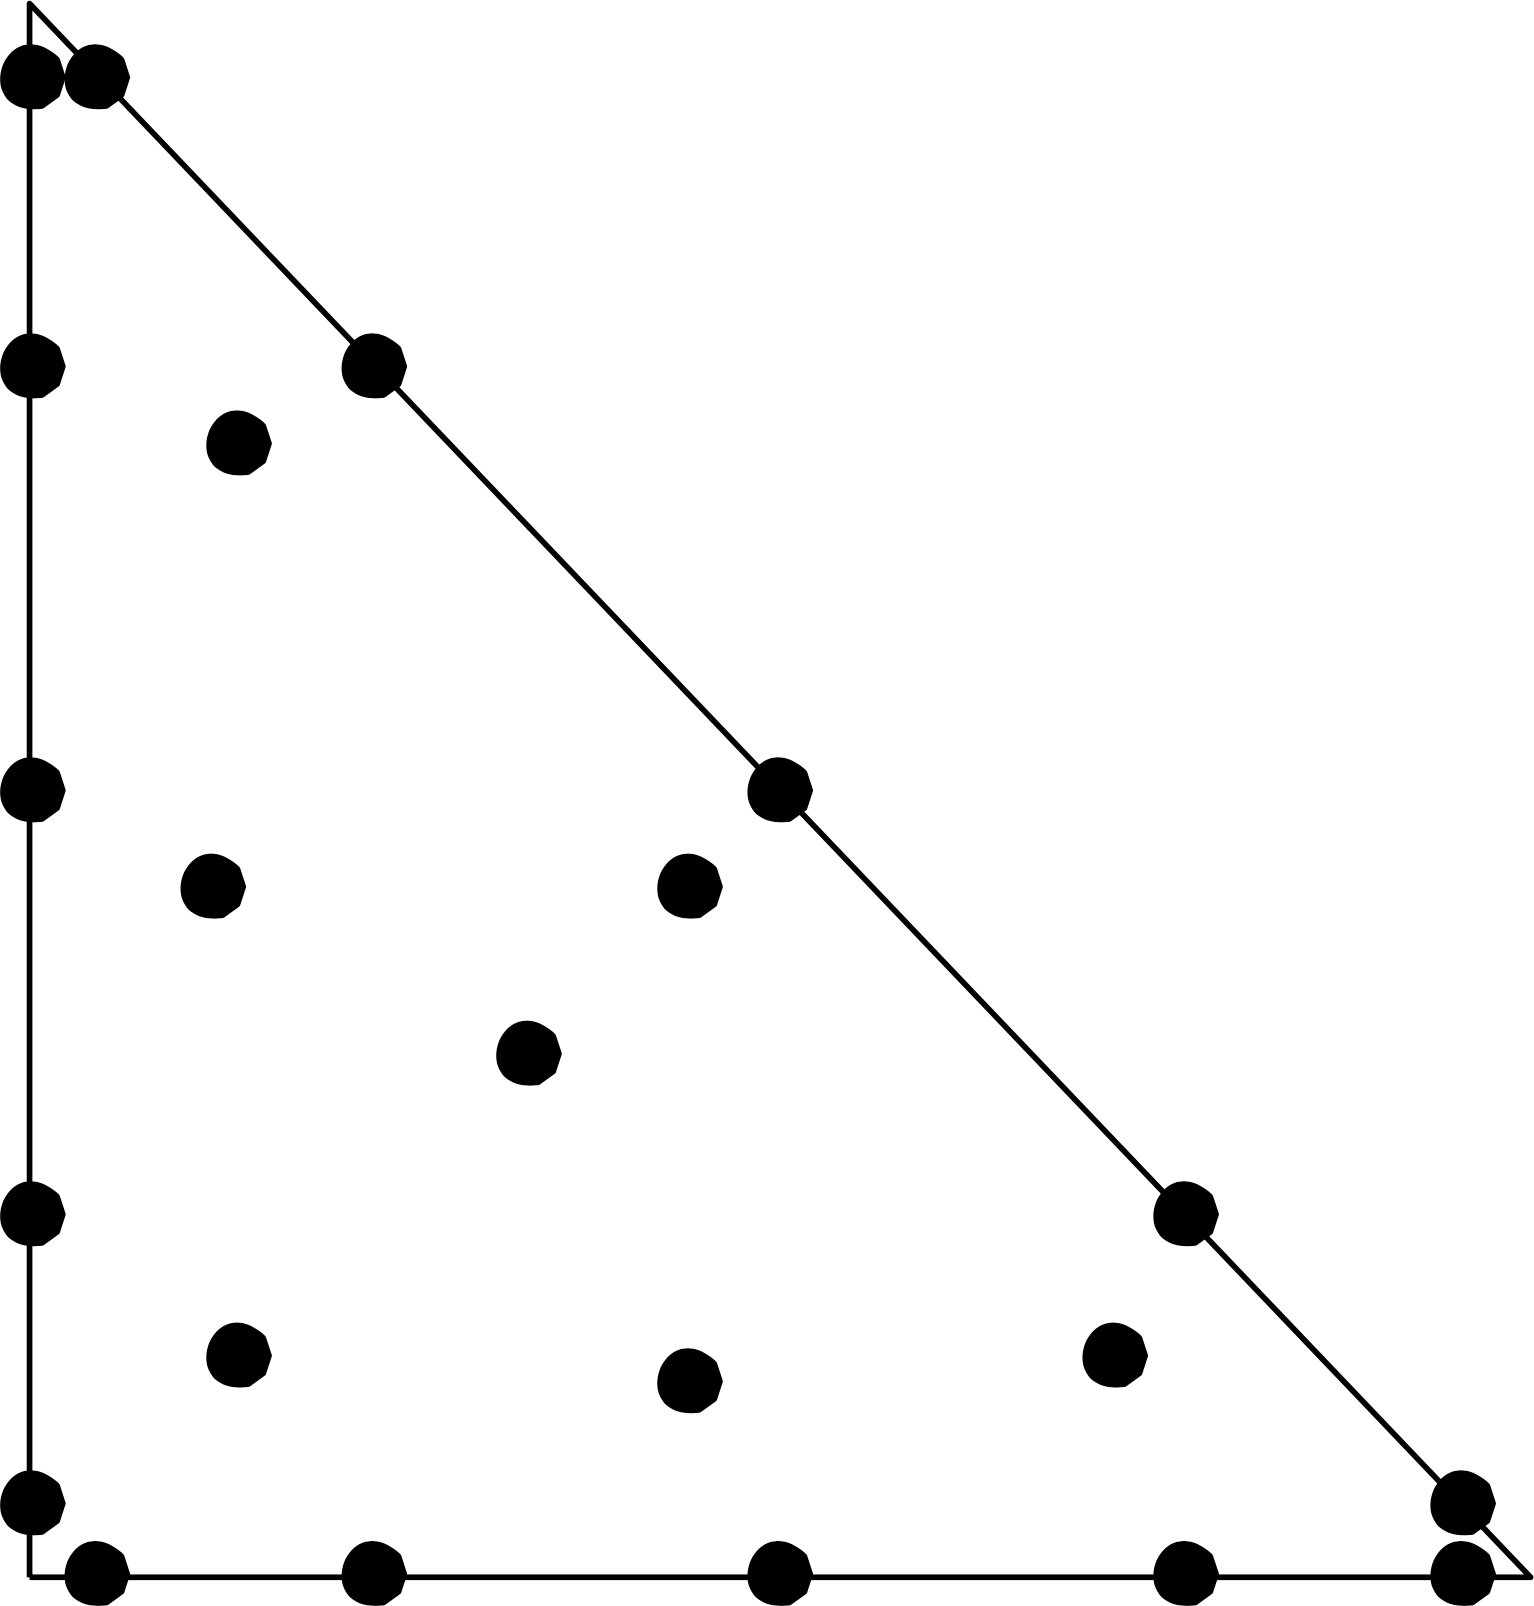
\includegraphics[height=.285\textheight]{figs/chenShuNodes.png}}
%\hspace{2.5em}
%\subfloat[Non-SBP nodes ($N=4$, 15 pts)]{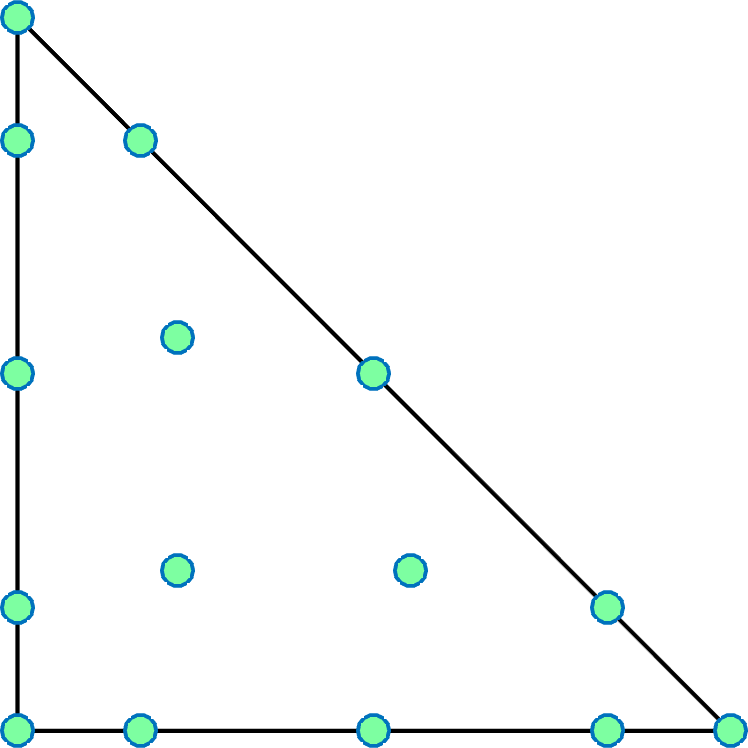
\includegraphics[height=.285\textheight]{figs/triNodesN4.png}}
%\endgroup
%%\caption{Dif.}
%\end{figure}
%
%\let\thefootnote\relax\footnotetext{\tiny Fisher and Carpenter (2013). \textit{High-order ES finite difference schemes for nonlinear conservation laws: Finite domains.} }
%%\let\thefootnote\relax\footnotetext{\tiny Carpenter et al.\ (2014). \textit{Entropy stable spectral collocation schemes for the NS equations: discontinuous interfaces.}}
%\let\thefootnote\relax\footnotetext{\tiny Gassner, Winters, and Kopriva (2016). \textit{Split form nodal DG schemes with SBP property for the comp.\ Euler equations.}}
%\let\thefootnote\relax\footnotetext{\tiny Chen and Shu (2017). \textit{ES high order DG methods with suitable quadrature rules for hyperbolic conservation laws.}}
%
%}

% =================================================

%\frame{
%\frametitle{Challenges for summation-by-parts formulations (SBP)}
%\setcounter{subfigure}{0}
%\begin{itemize} 
%\item Construction using \note{nodal collocation} at quadrature points.  
%\item Need at least $2N-1$ accurate volume and surface quadrature! 
%\item Difficult to generalize beyond polynomial DG (splines, pyramids, etc).
%\end{itemize}
%\vspace{-.5em}
%\begin{figure}
%\centering
%\begingroup
%\captionsetup[subfloat]{width=.3\textwidth}
%\subfloat[Tensor product SBP nodes (GLL quadrature)]{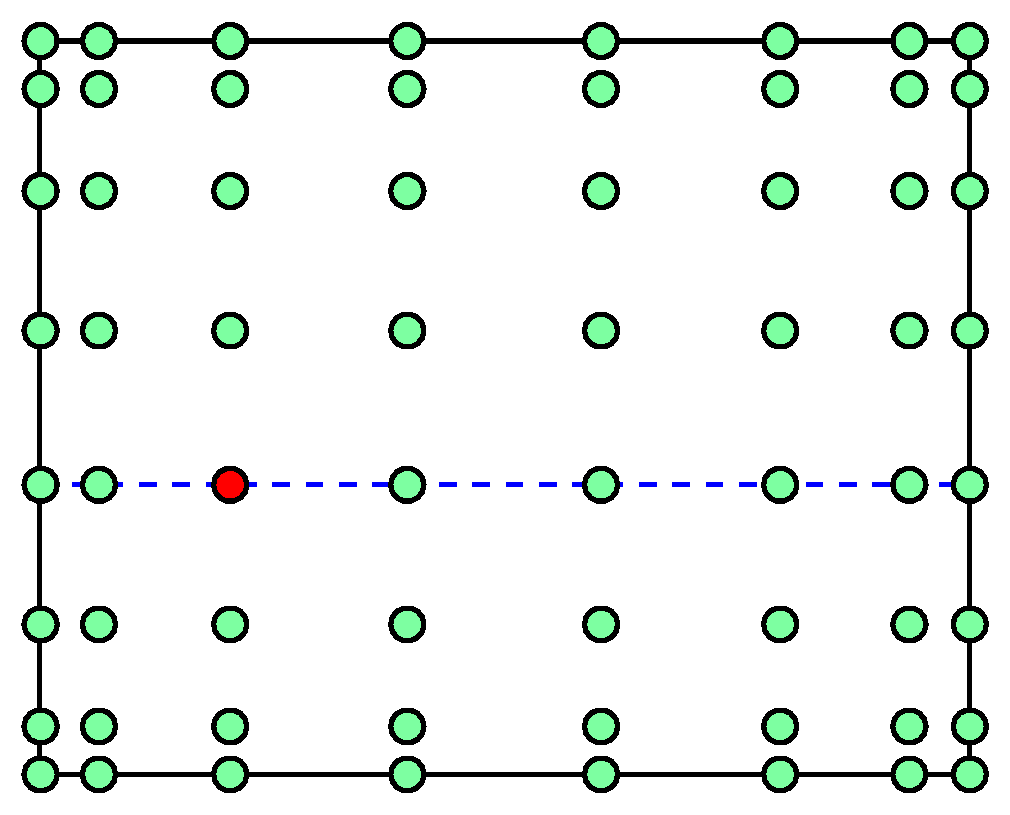
\includegraphics[width=.32\textwidth]{figs/SEM_stencil_1.pdf}}
%\hspace{1em}
%\subfloat[Interpolation nodes ($N=4$, 15 pts)]{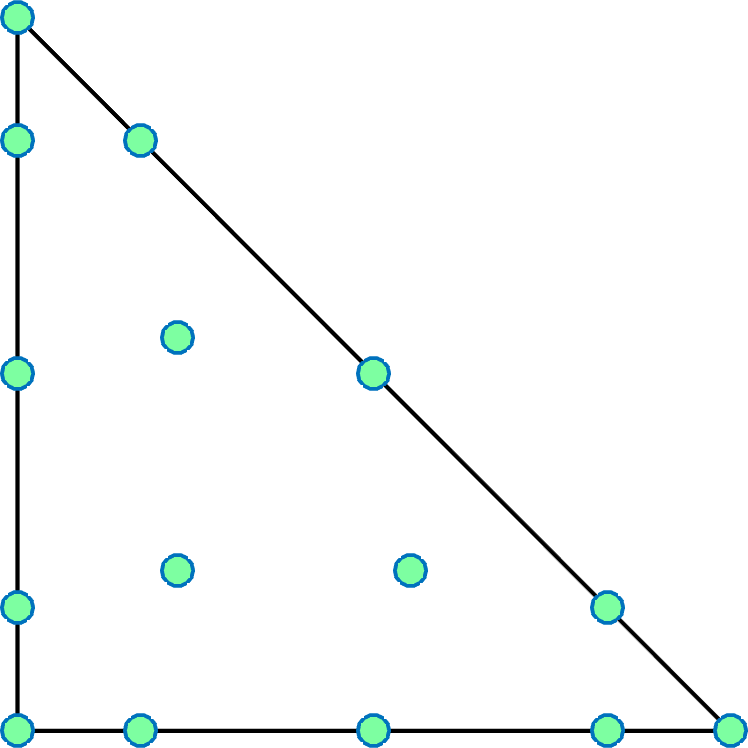
\includegraphics[width=.25\textwidth]{figs/triNodesN4.png}}
%\hspace{.5em}
%\subfloat[Diag-norm SBP nodes ($N=4$, 22 pts)]{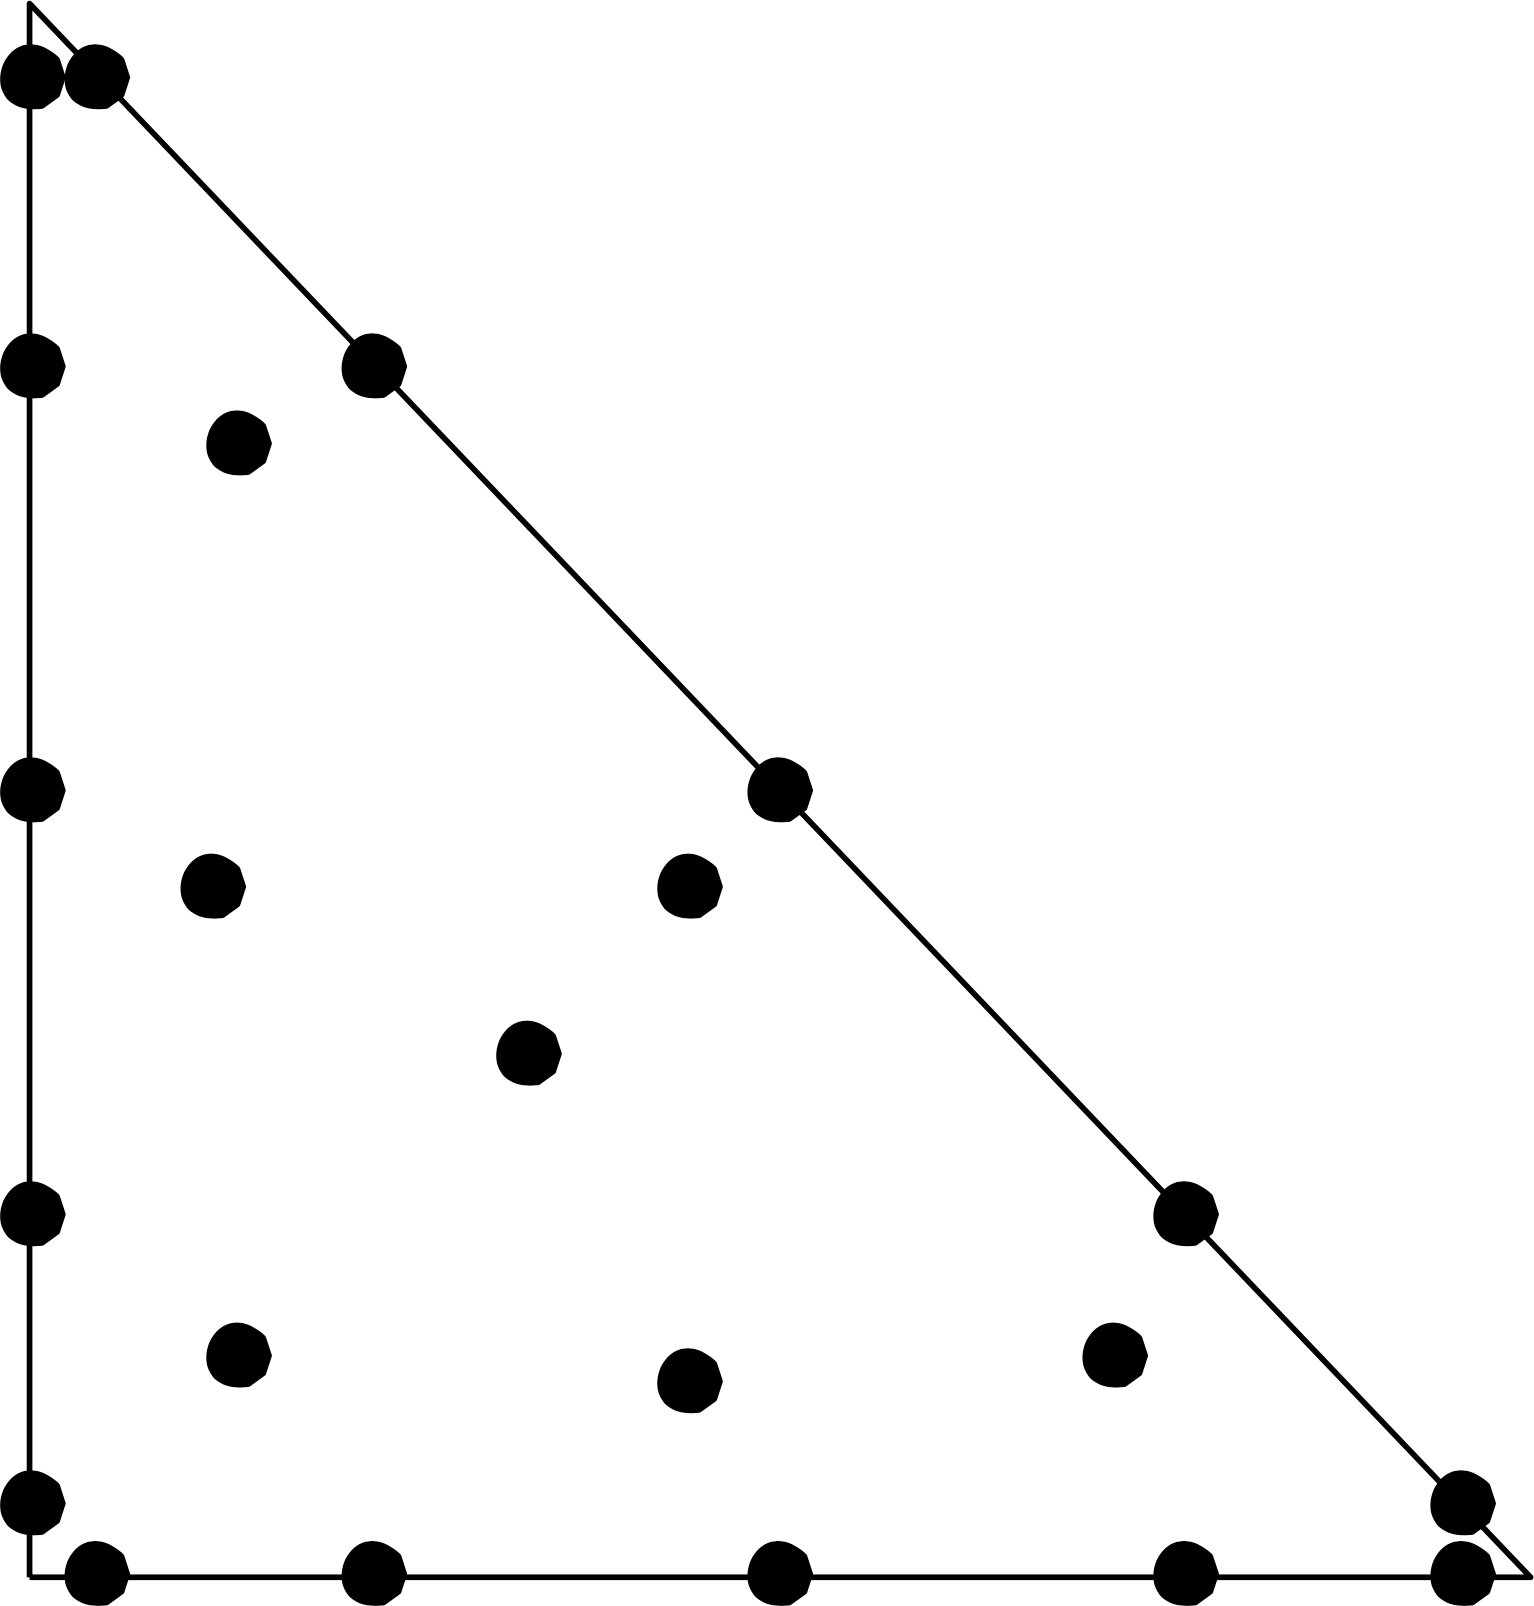
\includegraphics[width=.25\textwidth]{figs/chenShuNodes.png}}
%\endgroup
%%\caption{Dif.}
%\end{figure}
%
%\let\thefootnote\relax\footnotetext{\tiny Chen and Shu (2017). \textit{ES high order DG methods with suitable quadrature rules for hyperbolic conservation laws.}}
%\let\thefootnote\relax\footnotetext{\tiny Chan and Evans (2017). \textit{Multi-patch DG spline finite element methods for time-domain wave propagation}.}
%}


% =================================================

%\section{Flux differencing and discrete entropy conservation}
%\frame[noframenumbering]{
%\frametitle{Talk outline}
%\tableofcontents[currentsection]
%}

\frame{
\frametitle{Flux differencing: entropy conservative finite volume fluxes}

\begin{itemize}
\item<1-> Tadmor's entropy conservative (mean value) numerical flux 
\begin{align*}
\bm{f}_S(\bm{u},\bm{u}) &= \bm{f}(\bm{u}), \qquad \text{(consistency)} \\
\bm{f}_S(\bm{u},\bm{v}) &= \bm{f}_S(\bm{v},\bm{u}),\qquad \text{(symmetry)} \\
\LRp{\bm{v}_L - \bm{v}_R}^T \bm{f}\LRp{\bm{u}_L,\bm{u}_R} &= \psi_L - \psi_R, \qquad \text{(conservation)}.
\end{align*}
\item<2-> Example: entropy conservative flux for Burgers' equation 
\[
f_S(u_L,u_R) = \frac{1}{6}\LRp{u_L^2 + u_Lu_R + u_R^2}.
\]
\item<3-> Flux differencing: using finite volume numerical fluxes to evaluate high order derivatives in DG methods.
%\item<3-> Flux differencing for Burgers' equation: let $u_L = u(x), u_R = u(y)$
%\begin{align*}
%&f_S(u(x),u(y)) = \frac{1}{6}\LRp{u(x)^2 + u(x)u(y) + u(y)^2},\\
%&\pd{{f}({u})}{x} \Longrightarrow \note{\LRu{2\pd{f_S\LRp{u(x),u(y)}}{x}}_{y=x}} = \frac{1}{3}\pd{u^2}{x} + \frac{1}{3}u\pd{u}{x} + \frac{1}{3}u^2\cancel{\pd{1}{x}}.
%\end{align*}
\end{itemize}

\let\thefootnote\relax\footnotetext{\tiny Tadmor, Eitan (1987). \textit{The numerical viscosity of entropy stable schemes for systems of conservation laws. I.}}
}

\frame{
\frametitle{Flux differencing: recovering split formulations}
\begin{itemize}
\item<1-> Entropy conservative flux for Burgers' equation 
\[
f_S(u_L,u_R) = \frac{1}{6}\LRp{u_L^2 + u_Lu_R + u_R^2}.
\]
\item<1-> Flux differencing: let $u_L = u(x), u_R = u(y)$
\begin{align*}
\pd{{f}({u})}{x} &\Longrightarrow \note{\LRu{2\pd{f_S\LRp{u(x),u(y)}}{x}}_{y=x}}
\end{align*}
\item<2-> Recovering the Burgers' split formulation
\begin{align*}
f_S(u(x),u(y)) &= \frac{1}{6}\LRp{u(x)^2 + u(x)u(y) + u(y)^2}\\
\LRu{2\pd{f_S\LRp{u(x),u(y)}}{x}}_{y=x} &= \frac{1}{3}\pd{u^2}{x} + \frac{1}{3}u\pd{u}{x} + \frac{1}{3}u^2\cancel{\pd{1}{x}}.
\end{align*}
\end{itemize}
}

\frame{
\frametitle{Flux differencing: beyond split formulations}
\begin{itemize}
\item Fluxes do not necessarily correspond to split formulations!  
\vspace{.5em}
\item Example: entropy conservative flux for 1D compressible Euler
\begin{align*}
f^1_S(\bm{u}_L,\bm{u}_R) &= \avg{\rho}^{\log} \avg{u}\\
f^2_S(\bm{u}_L,\bm{u}_R) &= \frac{\avg{\rho}}{2\avg{\beta}} + \avg{u}f^1_S\\
f^3_S(\bm{u}_L,\bm{u}_R) &= f^1_S\LRp{\frac{1}{2(\gamma-1)\avg{\beta}^{\log}} - \frac{1}{2}\avg{u^2}} + \avg{u}f^2_S,
\end{align*}
%\vspace{.5em}
\item Logarithmic mean and ``inverse temperature'' $\beta$
\[
\avg{u}^{\log} = \frac{u_L - u_R}{\log{u_L}- \log{u_R}}, \qquad \beta = \frac{\rho}{2p}.
\]
\end{itemize}

\let\thefootnote\relax\footnotetext{\tiny Chandreshekar (2013),  \emph{Kinetic energy preserving and entropy stable FV schemes for comp.\ Euler and NS equations.}}
}

\frame{
\frametitle{Flux differencing: implementational details}
\begin{itemize}
%\item Flux differencing necessary for general nonlinear conservation laws (compressible Euler), not for split forms (Burgers, shallow water).  
\item Define ${\bm{F}_S}$ as evaluation of $\bm{f}_S$ at all combinations of quadrature points
\[
\LRp{\bm{F}_S}_{ij} = \LRp{u(\bm{x}_i),u(\bm{x}_j)}, \qquad \bm{x} = \LRs{\bm{x}^q,\bm{x}^f}^T.
\]
\item Replace $\pd{}{x}$ with $\bm{D}_N$ + projection and lifting matrices.
\[
\LRu{2\pd{f_S\LRp{u(x),u(y)}}{x}}_{y=x} \Longrightarrow \LRs{\begin{array}{cc}
\bm{P}_q & \bm{L}_f\end{array}}
{\rm diag}{\LRp{2\bm{D}_N \bm{F}_S}}.
\]
\item Efficient \note{Hadamard product} reformulation of flux differencing (efficient on-the-fly evaluation of $\bm{F}_S$) 
\[
{\rm diag}{\LRp{2\bm{D}_N \bm{F}_S}} = \LRp{2\bm{D}_N \circ \bm{F}_S}\bm{1}.
\]
\end{itemize}

%\let\thefootnote\relax\footnotetext{\tiny Chandrashekar (2013). \textit{Kinetic energy preserving and entropy stable FV schemes for compressible Euler and NS equations.}}
}

%\frame{
%\frametitle{Entropy stable high order DG: implementation}
%
%\begin{itemize}
%\item Right hand side evaluation for explicit time-stepping:
%\begin{enumerate}
%\item Compute $L^2$ projection of entropy variables $P_N\LRp{\bm{v}(\bm{u})}$.
%\item Eval.\ conservative variables $\bm{u}(P_N\LRp{\bm{v}(\bm{u})})$ at quadrature points.
%\item Compute $\bm{RHS}(\bm{u}) = {\rm diag}\LRp{2\bm{D}^x_h \bm{f}_S\LRp{\bm{u}_x,\bm{u}_y}}$
%%\item Compute $\bm{RHS}(\bm{u}) = 2\LRp{\bm{D}_h \circ \bm{F}_S}\bm{1}$
%\end{enumerate}
%\vspace{1em}
%\item Efficient \note{Hadamard product} reformulation (low-memory evaluation)
%\begin{align*}
%\LRs{\begin{array}{c}
%\bm{P}_q\\
%\bm{L}_f\end{array}}
%{\rm diag}{\LRp{2\bm{D}_N \bm{F}_S}}.
%\] = 
%\end{align*}
%%\vspace{1em}
%%\item Simplifications for diag-norm SBP (nodal collocation): avoid computing projections, combine volume + surface operations.
%\end{itemize}
%}
%% =================================================

\frame{
\frametitle{Flux differencing: avoiding the chain rule} 

\begin{itemize}
\item Test with entropy variables $\tilde{\bm{v}}$, integrate, and use SBP property:
\[
\tilde{\bm{v}}^T\LRp{2\bm{Q}_N \circ \bm{F}_S}\bm{1} = \tilde{\bm{v}}^T\LRp{\LRp{
\LRs{\begin{array}{cc}
0 &\\
& \bm{W}_f\bm{n}
\end{array}}
 + \bm{Q}_N - \bm{Q}_N^T} \circ \bm{F}_S}\bm{1}.
\]
\item Only boundary terms appear in final estimate; volume terms become boundary terms using properties of $\LRp{\bm{F}_S}_{ij} = \bm{f}_S\LRp{\tilde{\bm{u}}_i,\tilde{\bm{u}}_j}$
\begin{overlayarea}{\textwidth}{.275\textheight}
\begin{align*}
\tilde{\bm{v}}^T\LRp{\LRp{\bm{Q}_N - \bm{Q}_N^T} \circ \bm{F}_S}\bm{1} 
&= \tilde{\bm{v}}^T\LRp{\bm{Q}_N \circ \bm{F}_S}\bm{1} - \bm{1}^T\LRp{\bm{Q}_N \circ \bm{F}_S}\tilde{\bm{v}}  \\
\only<1>{&= \sum_{i,j} \LRp{\bm{Q}_N}_{ij} \textcolor{red}{\LRp{\tilde{\bm{v}}_i - \tilde{\bm{v}}_j}^T\bm{f}_S\LRp{\tilde{\bm{u}}_i,\tilde{\bm{u}}_j}}.}
\only<2>{&= \sum_{i,j} \LRp{\bm{Q}_N}_{ij} \textcolor{red}{\LRp{\psi(\tilde{\bm{u}}_i)-\psi(\tilde{\bm{u}}_j)}.}}
\only<3>{&= \textcolor{red}{\bm{1}^T\bm{Q}_N \bm{\psi} - \bm{\psi}^T\bm{Q}_N\bm{1} = \bm{1}^T\bm{Q}_N \bm{\psi} }}
\only<4->{&= \textcolor{red}{\bm{1}^T\LRp{\bm{B}_N-\bm{Q}_N^T} \bm{\psi} = \bm{1}^T\bm{B}_N\bm{\psi}.
%\bm{1}^T\LRs{\begin{array}{cc}
%0 &\\
%& \bm{W}_f\bm{n}
%\end{array}}\bm{\psi}.
}}
%\only<3>{&= \sum_{i,j} \LRp{\bm{Q}_N}_{ij} \textcolor{red}{\LRp{\bm{v}_i - \bm{v}_j}^T\bm{f}_S\LRp{\bm{u}_i,\bm{u}_j}}.}
\end{align*}
\end{overlayarea}
%\item Let $\bm{v}_q$ be entropy variables at quadrature points.  Multiply by $\LRp{\bm{P}_q\bm{v}}^T\bm{M}$
%\[
%\bm{v}_q^T \bm{P}_q^T \bm{M} \td{\hat{\bm{u}}}{t} = \bm{v}_q^T \bm{W} \bm{V}_q \bm{M}^{-1}\bm{M} \td{\hat{\bm{u}}}{t} = \bm{v}_q^T \bm{W}  \td{\LRp{\bm{V}_q\hat{\bm{u}}}}{t} = .  
%\]
\item<5-> Proof requires $\tilde{\bm{v}} = \bm{v}(\tilde{\bm{u}})$; the entropy variables $\tilde{\bm{v}}$ must be a function of the conservative variables $\tilde{\bm{u}}$.%; modify conservative variables $\tilde{\bm{u}}$ to ensure test function $\bm{v}(\tilde{\bm{u}}) = P_N\bm{v}(\bm{u}) \in P^N$.
%\item<4-> Proof requires $\bm{v} = \bm{v}(\bm{u})$ \textcolor{red}{pointwise}; modify conservative variables $\tilde{\bm{u}}$ to ensure test function $\bm{v}(\tilde{\bm{u}}) = P_N\bm{v}(\bm{u}) \in P^N$.
\end{itemize} 
}

\frame{
\frametitle{Modifying the conservative variables} 

\begin{itemize}
\item Conservative variables $\bm{u}_h$ and test functions are polynomial, but the entropy variables $\bm{v}(\bm{u}_h)\not\in P^N$!
\vspace{1em}
\item Evaluate flux $\bm{f}_S$ using \note{modified} conservative variables $\tilde{\bm{u}}$
\[
\tilde{\bm{u}} = \bm{u}\LRp{P_N\bm{v}(\bm{u}_h)}.
\]
%\vspace{1em}
\item \note{If $\bm{v}(\bm{u})$ is an invertible mapping}, this choice of $\tilde{\bm{u}}$ ensures that 
\[
\tilde{\bm{v}} = \bm{v}(\tilde{\bm{u}}) = P_N\bm{v}(\bm{u}_h) \in P^N.
\]
%\vspace{1em}
\item Local conservation w.r.t.\ a generalized Lax-Wendroff theorem.
\end{itemize}
\let\thefootnote\relax\footnotetext{\tiny Shi and Shu (2017). \emph{On local conservation of numerical methods for conservation laws}.}
}


\frame{
\frametitle{A discretely entropy conservative DG method}
\vspace{-1em}
%\begin{overlayarea}{\textwidth}{.9\textheight}d
\begin{theorem}[Chan 2018]
Let $\bm{u}_h(\bm{x}) = \sum_j \hat{\bm{u}}_j \phi_j(\bm{x})$ and $\tilde{\bm{u}} = \bm{u}\LRp{P_N\bm{v}}$.  Let $\hat{\bm{u}}$ locally solve 
\[
\td{\hat{\bm{u}}}{t} + \sum_{i=1}^d\LRs{\begin{array}{cc}
\bm{P}_q & \bm{L}_f\end{array}} \LRp{2\bm{D}^i_N \circ \bm{F}^i_S}\bm{1} + \bm{L}_f \LRp{\bm{f}^i_S(\tilde{\bm{u}}^+,\tilde{\bm{u}}) - \bm{f}^i(\tilde{\bm{u}})}\bm{n}_i = 0.
%\LRp{\pd{\bm{u}}{t} + \left.\LRp{2 D^x_h \bm{f}_S(\bm{u}_x,\bm{u}_y)}\right|_{y=x},\bm{w}}_{\Omega} = 0, \qquad \forall \bm{w}\in V_h.
\]
Assuming continuity in time, $\bm{u}_h(\bm{x})$ satisfies the quadrature form of
\[
\int_{\Omega} \pd{S(\bm{u}_h)}{t} + \sum_{i=1}^d\int_{\partial \Omega} \LRp{(P_N\bm{v})^T\bm{f}^i(\tilde{\bm{u}}) - \psi_i(\tilde{\bm{u}})} \bm{n}_i = 0.
\]
%\[
%\int_{\Omega} \pd{S}{t} + \int_{\partial \Omega} \bm{v}^T\bm{f}(\bm{u}) - \psi(\bm{u}) = 0.
%\]
\end{theorem} 
%\only<5>{
%\vspace{-.25em}
\begin{itemize}
%\item Note: $\bm{u}\in P^N$, but $\bm{v}(\bm{u}) \not\in P^N$! 
% Entropy conservation uses $L^2$-\note{projected} entropy variables $P_N \bm{v}$ and redefined $\tilde{\bm{u}} = \bm{u}\LRp{P_N\bm{v}}$!
\item Can modify interface flux (e.g.\ Lax-Friedrichs) for entropy \note{dissipation}. 
\end{itemize}

\let\thefootnote\relax\footnotetext{\tiny Chan (2018). \textit{On discretely entropy conservative and entropy stable discontinuous Galerkin methods.}}
}

%
%\frame{
%\frametitle{Local conservation}
%
%\begin{itemize}
%\item Flux differencing 
%\item \note{Describe local conservation}
%\end{itemize}
%\let\thefootnote\relax\footnotetext{\tiny Shi and Shu (2017). \emph{On local conservation of numerical methods for conservation laws}.}
%}

\frame{
\frametitle{Curved meshes and stability}
\vspace{-.5em}
\begin{figure}
\centering
\subfloat[Curved mesh]{\raisebox{.75em}{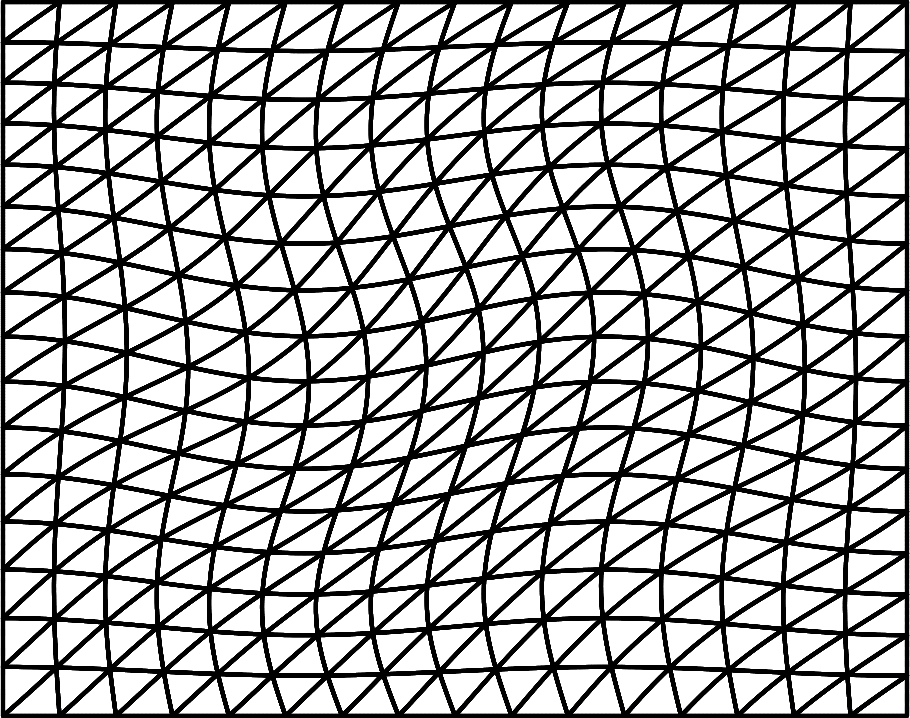
\includegraphics[width=.29\textwidth]{figs/advecMesh.png}}}
\hspace{.25em}
\subfloat[Aliased solution]{\includegraphics[width=.31\textwidth]{figs/advecAlias.png}}
\hspace{.25em}
\subfloat[Energy growth]{\includegraphics[width=.32\textwidth]{figs/advecEnergy.png}}
%\caption*{}
\end{figure}
\begin{itemize}
\item Necessary for high order accuracy on curved geometries, but can produce ``aliasing'' instabilities and energy growth.
\item Geometric terms $J, \bm{G}_{ij}$ vary spatially over each element %act like variable coefficients
\[
\pd{u}{x_i} = \sum_{j=1}^d\bm{G}_{ij} \pd{u}{\hat{x}_j}, \qquad \bm{G}_{ij} = \pd{\hat{x}_j}{x_i}, \qquad J = \frac{1}{{\rm det}(\bm{G})}.
\]
\end{itemize}
}

\frame{
\frametitle{Curved meshes: geometric terms}

\begin{itemize}
\item Rewrite derivatives in \note{split form} with scaled geometric terms
\[
J\pd{u}{x_i} = \frac{1}{2} \sum_{j=1}^d \LRp{J \bm{G}_{ij} \pd{u}{\hat{x}_j} + \pd{\LRp{J\bm{G}_{ij} u}}{\hat{x}_j}}, \qquad \sum_{j=1}^d \pd{\LRp{J\bm{G}_{ij}}}{\hat{x}_j} = 0.
\]
\item Define physical matrices in terms of reference matrices $\hat{\bm{D}}^j_N$ 
\[
%\bm{D}^i_N = \sum_{i=1}^d \LRp{\hat{\bm{D}}^j_N \circ \avg{\bm{JG}_{ij}}}, \qquad \LRp{\avg{\bm{JG}_{ij}}}_{mn} =  \frac{\LRp{\bm{JG}_{ij}}_m+\LRp{\bm{JG}_{ij}}_n}{2}.
\bm{D}^i_N = \frac{1}{2} \sum_{i=1}^d \LRp{{\rm diag}\LRp{\bm{JG}_{ij}}\hat{\bm{D}}^j_N + \hat{\bm{D}}^j_N{\rm diag}\LRp{\bm{JG}_{ij}} }.
\]
\item Proof of discrete entropy conservation requires $\bm{D}^i_N \bm{1}=0$.  Must ensure geometric terms satisfy geometric conservation law (GCL).  
%\begin{align*}
%\bm{D}^i_N \bm{1} &= 
%\frac{1}{2} \sum_{j=1}^d \hat{\bm{D}}^j_N \LRp{\bm{JG}_{ij}} + {\rm diag}\LRp{\bm{JG}_{ij}}\hat{\bm{D}}^j_N \bm{1} = 0\\ &\Longrightarrow \sum_{j=1}^d \hat{\bm{D}}^j_N \LRp{\bm{JG}_{ij}}  = 0.
%\end{align*}
\[
\bm{D}^i_N \bm{1} =  0 \Longrightarrow \sum_{j=1}^d \hat{\bm{D}}^j_N \LRp{\bm{JG}_{ij}}  = 0.
\]
\end{itemize}

\let\thefootnote\relax\footnotetext{\tiny Thomas and Lombard (1979).  Geometric Conservation Law and Its Application to Flow Computations on Moving Grids.}
\let\thefootnote\relax\footnotetext{\tiny Kopriva (2006).  Metric identities and the discontinuous spectral element method on curvilinear meshes.}

}

\frame{
\frametitle{Curved meshes: weighted mass matrices}

\begin{itemize}
\item Weighted mass matrix $\bm{M}_J$ on $D^k$, weighted $L^2$ projection $\bm{P}^k_q$
\[
\LRp{\bm{M}_J}_{ij} = \int_{\hat{D}}\phi_j \phi_i J \diff{\hat{\bm{x}}}, \qquad \bm{P}^k_q = \LRp{\bm{M}_J}^{-1}\bm{V}_q^T\bm{W}{\rm diag}\LRp{\bm{J}}.
\]
\item Avoid $\bm{M}_J^{-1}$: generalized mass lumping, weight-adjusted mass matrix 
\begin{gather*}
\bm{M}_J \approx \bm{M}\bm{M}_{1/J}^{-1}\bm{M}, \qquad \LRp{\bm{M}\bm{M}_{1/J}^{-1}\bm{M}}^{-1} = \bm{M}^{-1}\bm{M}_{1/J}\bm{M}^{-1}
\end{gather*}
\item Low-storage matrix-free application of $\bm{M}_{1/J}$ using quadrature.
\vspace{.25em}
\item For discrete entropy conservation, use weight-adjusted projection 
\[
\tilde{P}^k_N u = P_N \LRp{\frac{1}{J}P_N\LRp{uJ}}.
\]
\end{itemize}

\let\thefootnote\relax\footnotetext{\tiny Chan, Wilcox (in preparation). \textit{On discretely entropy stable weight-adjusted DG methods: curvilinear meshes}.}
\let\thefootnote\relax\footnotetext{\tiny Chan, Hewett, and Warburton (2016). \textit{Weight-adjusted discontinuous Galerkin methods: curvilinear meshes}.}
}


%% =================================================

\section{Numerical experiments}

\frame[noframenumbering]{
\frametitle{Talk outline}
\tableofcontents[currentsection]
}

\frame{
\frametitle{1D compressible Euler equations}

\begin{itemize}
\item Inexact Gauss-Legendre-Lobatto (GLL) vs Gauss (GQ) quadratures. 
\item Entropy conservative (EC) and Lax-Friedrichs (LF) fluxes.  
\item No additional stabilization, filtering, or limiting.
%\item $L^2$ rates: odd/even decoupling for EC, $O(h^{N+1})$ for LF.
\end{itemize} 
\vspace{-1em}
\begin{figure}
\centering
\subfloat[Entropy conservative flux]{
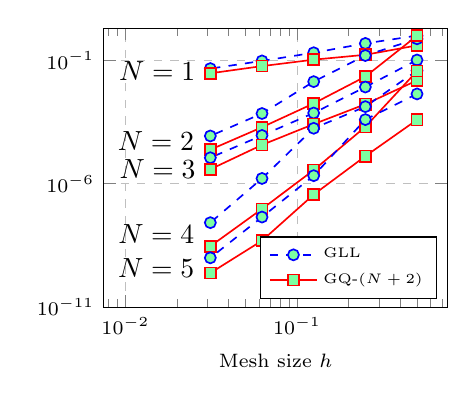
\begin{tikzpicture}
\begin{loglogaxis}[
    width=.49\textwidth,
    xlabel={Mesh size $h$},
%    ylabel={$L^2$ errors}, 
    xmin=.0075, xmax=.75,
    ymin=1e-11, ymax=2,
    legend pos=south east, legend cell align=left, legend style={font=\tiny},	
    xmajorgrids=true, ymajorgrids=true, grid style=dashed,
    legend entries={GLL,GQ-$(N+2)$}    
]
\pgfplotsset{
cycle list={{blue, dashed, mark=*}, {red, mark=square*}}
}
%\addlegendimage{no markers,blue}
%\addlegendimage{no markers,red}

\addplot+[semithick, mark options={solid, fill=markercolor}]
% N = 1, tau = 0.000000 =======================
coordinates{(0.5,1)(0.25,0.485059)(0.125,0.203599)(0.0625,0.0947163)(0.03125,0.0463705)};
\addplot+[semithick, mark options={solid, fill=markercolor}]
%N = 1, tau = 0.000000 =======================
coordinates{(0.5,0.402314)(0.25,0.167917)(0.125,0.106574)(0.0625,0.058359)(0.03125,0.0298728)}
[yshift=1pt] node[left, pos=1.025, color=black] {$N = 1$};


\addplot+[semithick, mark options={solid, fill=markercolor}]
% N = 2, tau = 0.000000 =======================
coordinates{(0.5,0.746606)(0.25,0.156701)(0.125,0.0137392)(0.0625,0.000701926)(0.03125,8.64531e-05)};
\addplot+[semithick, mark options={solid, fill=markercolor}]
%N = 2, tau = 0.000000 =======================
coordinates{(0.5,0.993771)(0.25,0.0219437)(0.125,0.00180028)(0.0625,0.000194939)(0.03125,2.4045e-05)}
[yshift=4pt] node[left, pos=1.025, color=black] {$N = 2$};


\addplot+[semithick, mark options={solid, fill=markercolor}]
% N = 3, tau = 0.000000 =======================
coordinates{(0.5,0.103299)(0.25,0.00829887)(0.125,0.00073573)(0.0625,9.05975e-05)(0.03125,1.13596e-05)};
\addplot+[semithick, mark options={solid, fill=markercolor}]
%N = 3, tau = 0.000000 =======================
coordinates{(0.5,0.0154054)(0.25,0.00167426)(0.125,0.000260859)(0.0625,3.76182e-05)(0.03125,3.86238e-06)}
[yshift=1pt] node[left, pos=1.025, color=black] {$N = 3$};

\addplot+[semithick, mark options={solid, fill=markercolor}]
% N = 4, tau = 0.000000 =======================
coordinates{(0.5,0.0385542)(0.25,0.00133048)(0.125,0.000176663)(0.0625,1.64135e-06)(0.03125,2.66024e-08)};
\addplot+[semithick, mark options={solid, fill=markercolor}]
%N = 4, tau = 0.000000 =======================
coordinates{(0.5,0.0367592)(0.25,0.000202817)(0.125,3.57758e-06)(0.0625,9.58294e-08)(0.03125,2.94985e-09)}[yshift=6pt] node[left, pos=1.025, color=black] {$N = 4$};

\addplot+[semithick, mark options={solid, fill=markercolor}]
% N = 5, tau = 0.000000 =======================
coordinates{(0.5,0.00436131)(0.25,0.00039846)(0.125,2.1282e-06)(0.0625,4.49046e-08)(0.03125,9.99912e-10)};
\addplot+[semithick, mark options={solid, fill=markercolor}]
%N = 5, tau = 0.000000 =======================
coordinates{(0.5,0.000390565)(0.25,1.31188e-05)(0.125,3.6544e-07)(0.0625,4.95271e-09)(0.03125,2.42763e-10)}
[yshift=3pt] node[left, pos=1.025, color=black] {$N = 5$};

%\legend{$N=1$,$N=2$,$N=3$,$N=4$,$N=5$}
\end{loglogaxis}
\end{tikzpicture}
}
\subfloat[With Lax-Friedrichs penalization]{
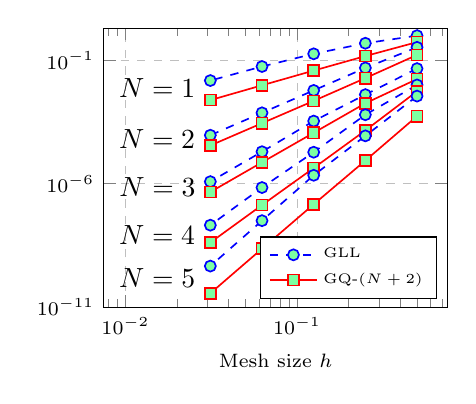
\begin{tikzpicture}
\begin{loglogaxis}[
    width=.49\textwidth,
    xlabel={Mesh size $h$},  %ylabel={$L^2$ errors}, 
    xmin=.0075, xmax=.75,
    ymin=1e-11, ymax=2,
    legend pos=south east, legend cell align=left, legend style={font=\tiny},	
    xmajorgrids=true, ymajorgrids=true, grid style=dashed,
    legend entries={GLL,GQ-$(N+2)$}
] 
\pgfplotsset{
cycle list={{blue, dashed, mark=*}, {red, mark=square*}}
}
%\pgfplotsset{cycle list={{blue, dashed, mark=*}, {red, mark=square*}}}

\addplot+[semithick, mark options={solid, fill=markercolor}]
% N = 1, tau = 0.500000 =======================
coordinates{(0.5,1)(0.25,0.4932)(0.125,0.183839)(0.0625,0.0562398)(0.03125,0.0151873)};
\addplot+[semithick, mark options={solid, fill=markercolor}]
%N = 1, tau = 0.500000 =======================
coordinates{(0.5,0.547558)(0.25,0.148981)(0.125,0.0384647)(0.0625,0.00974763)(0.03125,0.00244539)}
[yshift=5pt] node[left, pos=1.025, color=black] {$N = 1$};

\addplot+[semithick, mark options={solid, fill=markercolor}]	
% N = 2, tau = 0.500000 =======================
coordinates{(0.5,0.336817)(0.25,0.04941)(0.125,0.00605428)(0.0625,0.000748842)(0.03125,9.25456e-05)};
\addplot+[semithick, mark options={solid, fill=markercolor}]
%N = 2, tau = 0.500000 =======================
coordinates{(0.5,0.165807)(0.25,0.0190013)(0.125,0.00227903)(0.0625,0.00028425)(0.03125,3.54865e-05)}
[yshift=3pt] node[left, pos=1.025, color=black] {$N = 2$};


% N = 3, tau = 0.500000 =======================
\addplot+[semithick, mark options={solid, fill=markercolor}]
coordinates{(0.5,0.0463242)(0.25,0.00408748)(0.125,0.000346831)(0.0625,1.99064e-05)(0.03125,1.22357e-06)};
\addplot+[semithick, mark options={solid, fill=markercolor}]
%N = 3, tau = 0.500000 =======================
coordinates{(0.5,0.0174194)(0.25,0.00182234)(0.125,0.000116147)(0.0625,7.39839e-06)(0.03125,4.6305e-07)}
[yshift=3pt] node[left, pos=1.025, color=black] {$N = 3$};

\addplot+[semithick, mark options={solid, fill=markercolor}]
% N = 4, tau = 0.500000 =======================
coordinates{(0.5,0.0100716)(0.25,0.000625923)(0.125,1.89866e-05)(0.0625,7.03865e-07)(0.03125,2.10265e-08)};
\addplot+[semithick, mark options={solid, fill=markercolor}]
%N = 4, tau = 0.500000 =======================
coordinates{(0.5,0.00556743)(0.25,0.000144595)(0.125,4.33972e-06)(0.0625,1.37151e-07)(0.03125,4.16335e-09)}
[yshift=4pt] node[left, pos=1.025, color=black] {$N = 4$};


\addplot+[semithick, mark options={solid, fill=markercolor}]
% N = 5, tau = 0.500000 =======================
coordinates{(0.5,0.00356628)(0.25,8.73125e-05)(0.125,2.20528e-06)(0.0625,3.20127e-08)(0.03125,4.63639e-10)};
\addplot+[semithick, mark options={solid, fill=markercolor}]
%N = 5, tau = 0.500000 =======================
coordinates{(0.5,0.000547621)(0.25,8.7194e-06)(0.125,1.47105e-07)(0.0625,2.34345e-09)(0.03125,3.65306e-11)}
[yshift=7pt] node[left, pos=1.025, color=black] {$N = 5$};

\end{loglogaxis}
\end{tikzpicture}
}
%\caption*{$L^2$ errors under mesh refinement for entropy conservative and Lax-Friedrichs fluxes under both Gauss-Legendre-Lobatto (GLL) and over-integrated $(N+2)$ point Gauss quadrature (GQ-$(N+2)$).}
\label{fig:convergence}
\end{figure}

}

\frame{
\frametitle{Conservation of entropy: fully discrete schemes}
\setcounter{subfigure}{0}

\vspace{.5em}
\begin{itemize}
\item Entropy conservation: \textit{semi-discrete}, not fully discrete.
\item $\Delta S(\bm{u}) = \LRb{S(\bm{u}(x,t))-S(\bm{u}(x,0))} \rightarrow 0$ as as $\Delta t \rightarrow 0$.
\end{itemize}
\vspace{-.5em}
\begin{figure}
\centering
\subfloat[$\Delta S(\bm{u})$ for various $\Delta t$]{\includegraphics[width=.445\textwidth]{figs/dS_ECLF.png}}
\hspace{1em}
\subfloat[$\rho(x), u(x)$ ($N=4, K = 16$)]{\includegraphics[width=.46\textwidth]{figs/sol_ECLF.png}}
\caption*{Solution and change in entropy $\Delta S(\bm{u})$ for entropy conservative (EC) and Lax-Friedrichs (LF) fluxes (using GQ-$(N+2)$ quadrature). }
\end{figure}
}

\frame{
\frametitle{1D Sod shock tube}

\begin{itemize}
\item Circles are cell averages.
\item CFL of .125 used for both GLL-$(N+1)$and GQ-$(N+2)$.
\end{itemize}
\begin{figure}
\centering
\only<1>{\includegraphics[width=.8\textwidth]{figs/sodGLL.png}\caption*{$N=4, K = 32$, $(N+1)$ point Gauss-Lobatto-Legendre quadrature.}}
\only<2>{\includegraphics[width=.8\textwidth]{figs/sodGQ2.png}\caption*{$N=4, K = 32$, $(N+2)$ point Gauss quadrature.}}
\end{figure}
}


\frame{
\frametitle{1D sine-shock interaction}

\begin{itemize}
\item GQ-$(N+2)$ needs smaller CFL (.05 vs .125) for stability.  
\end{itemize}

\begin{figure}
\centering
\only<1>{\includegraphics[width=.8\textwidth]{figs/sineShockGLL.png}\caption*{$N=4, K = 40, CFL = .05$, $(N+1)$ point Gauss-Lobatto-Legendre quadrature.}}
\only<2>{\includegraphics[width=.8\textwidth]{figs/sineShockGQ2.png}\caption*{$N=4, K = 40, CFL = .05$, $(N+2)$ point Gauss quadrature.}}
\end{figure}
}

\frame{
\frametitle{On CFL restrictions}

\begin{itemize}
\item For GLL-$(N+1)$ quadrature, $\tilde{\bm{u}} = \bm{u}\LRp{P_N \bm{v}} = \bm{u}$ at GLL points.
\item For GQ-$(N+2)$, discrepancy between $L^2$ projection and interpolation.
\item Still need \note{positivity} of thermodynamic quantities for stability!
\end{itemize}
\vspace{-1em}
\begin{figure}
\centering
\subfloat[${v}_3(x), \LRp{P_N v_3}(x)$]{\includegraphics[width=.45\textwidth]{figs/sineShockQ3Compare.png}}
\hspace{1em}
\subfloat[$\rho(x), \rho\LRp{\LRp{P_N \bm{v}}(x)}$]{\includegraphics[width=.44\textwidth]{figs/sineShockDensityCompare.png}}
\end{figure}
}


%\frame{
%\frametitle{  two-dimensional curvilinear meshes}
%\setcounter{subfigure}{0}
%
%\only<1>{
%\begin{itemize}
%\item Vortex problem at $T = 5$, $\Omega = [0,20]\times [-5,5]$, CFL = .25.  
%\item Avoid weighted mass inverse using a \emph{weight-adjusted} approximation.
%%\[
%%\bm{M}_{J}^{-1} \approx \hat{\bm{M}}^{-1} \bm{M}_{1/J} \hat{\bm{M}}^{-1}.
%%\]
%\end{itemize}
%\let\thefootnote\relax\footnotetext{\tiny Chan, Hewett, and Warburton (2016). \textit{Weight-adjusted discontinuous Galerkin methods: curvilinear meshes}.}
%}
%\only<2>{
%$L^2$ error converges at $O(h^{N+1})$ up to time-stepper accuracy (LSRK-45).
%}
%
%\begin{figure}
%\centering
%\only<1>{
%\subfloat[Uniform mesh]{\includegraphics[width=.425\textwidth]{figs/vortexMeshUniform.png}}
%\hspace{1em}
%\subfloat[Warped mesh]{\includegraphics[width=.425\textwidth]{figs/vortexMeshCurved.png}}
%}
%\only<2>{
%%\vspace{-1em}
%\subfloat[Degrees $N=1, N= 3$]{\begin{tikzpicture}
%%\subfloat{\begin{tikzpicture}
%\begin{loglogaxis}[
%    width=.49\textwidth,
%    xlabel={Mesh size $h$},  ylabel={$L^2$ errors}, 
%    xmin=.075, xmax=7,
%    ymin=1e-5, ymax=1,   
%    legend pos = south east, legend cell align=left, legend style={font=\tiny},	
%    xmajorgrids=true, ymajorgrids=true, grid style=dashed,
%    legend entries={Affine, Curved}
%] 
%\pgfplotsset{
%cycle list={{blue, dashed, mark=*}, {red, mark=square*}}
%}
%%\pgfplotsset{cycle list={{blue, dashed, mark=*}, {red, mark=square*}}}
%\addplot+[semithick, mark options={solid, fill=markercolor}]
%coordinates{(5,0.152443)(2.5,0.509207)(1.25,0.445656)(0.625,0.166519)(0.3125,0.036208)};
%\addplot+[semithick, mark options={solid, fill=markercolor}]
%coordinates{(5,0.380788)(2.5,0.636067)(1.25,0.432155)(0.625,0.207952)(0.3125,0.059728)}
%[yshift=-2pt] node[left, pos=1.025, color=black] {$N = 1$};
%\logLogSlopeTriangle{0.45}{0.1}{0.72}{2.2}{blue}
%
%%\addplot+[semithick, mark options={solid, fill=markercolor}]
%%coordinates{(5,0.484478)(2.5,0.46951)(1.25,0.125591)(0.625,0.015585)(0.3125,0.001791)};
%%\addplot+[semithick, mark options={solid, fill=markercolor}]
%%coordinates{(5,0.670522)(2.5,0.468234)(1.25,0.189765)(0.625,0.035238)(0.3125,0.005043)}
%%[yshift=-1pt] node[left, pos=1.025, color=black] {$N = 2$};
%
%\addplot+[semithick, mark options={solid, fill=markercolor}]
%coordinates{(5,0.557086)(2.5,0.260022)(1.25,0.042815)(0.625,0.003611)(0.3125,0.000213)};
%\addplot+[semithick, mark options={solid, fill=markercolor}]
%coordinates{(5,0.54154)(2.5,0.312986)(1.25,0.07835)(0.625,0.00965)(0.3125,0.000739)}
%[yshift=-4pt] node[left, pos=1.025, color=black] {$N = 3$};
%\logLogSlopeTriangle{0.45}{0.1}{0.285}{4.084}{blue}
%
%%\addplot+[semithick, mark options={solid, fill=markercolor}]
%%coordinates{(5,0.463269)(2.5,0.169843)(1.25,0.017172)(0.625,0.000965)(0.3125,3.5e-05)};
%%\addplot+[semithick, mark options={solid, fill=markercolor}]
%%coordinates{(5,NaN)(2.5,0.247861)(1.25,0.043932)(0.625,0.002727)(0.3125,0.000118)}
%%[yshift=1pt] node[left, pos=1.025, color=black] {$N = 4$};
%
%\end{loglogaxis}
%\end{tikzpicture}
%}
%%\hspace{1em}
%\subfloat[Degrees $N=2, N= 4$]{\begin{tikzpicture}
%\begin{loglogaxis}[
%    width=.49\textwidth,
%    xlabel={Mesh size $h$},  ylabel={$L^2$ errors}, 
%    xmin=.075, xmax=7,
%    ymin=1e-5, ymax=1,
%    legend pos = north west, legend cell align=left, legend style={font=\tiny},	
%    xmajorgrids=true, ymajorgrids=true, grid style=dashed,
%    legend entries={Affine, Curved}
%] 
%\pgfplotsset{
%cycle list={{blue, dashed, mark=*}, {red, mark=square*}}
%}
%%\addplot+[semithick, mark options={solid, fill=markercolor}]
%%coordinates{(5,0.152443)(2.5,0.509207)(1.25,0.445656)(0.625,0.166519)(0.3125,0.036208)};
%%\addplot+[semithick, mark options={solid, fill=markercolor}]
%%coordinates{(5,0.380788)(2.5,0.636067)(1.25,0.432155)(0.625,0.207952)(0.3125,0.059728)}
%%[yshift=-2pt] node[left, pos=1.025, color=black] {$N = 1$};
%%\logLogSlopeTriangle{0.45}{0.05}{0.625}{2.2}{blue}
%
%\addplot+[semithick, mark options={solid, fill=markercolor}]
%coordinates{(5,0.484478)(2.5,0.46951)(1.25,0.125591)(0.625,0.015585)(0.3125,0.001791)};
%\addplot+[semithick, mark options={solid, fill=markercolor}]
%coordinates{(5,0.670522)(2.5,0.468234)(1.25,0.189765)(0.625,0.035238)(0.3125,0.005043)}
%[yshift=-3pt] node[left, pos=1.025, color=black] {$N = 2$};
%\logLogSlopeTriangle{0.45}{0.1}{0.465}{3.12}{blue}
%
%%\addplot+[semithick, mark options={solid, fill=markercolor}]
%%coordinates{(5,0.557086)(2.5,0.260022)(1.25,0.042815)(0.625,0.003611)(0.3125,0.000213)};
%%\addplot+[semithick, mark options={solid, fill=markercolor}]
%%coordinates{(5,0.54154)(2.5,0.312986)(1.25,0.07835)(0.625,0.00965)(0.3125,0.000739)}
%%[yshift=-4pt] node[left, pos=1.025, color=black] {$N = 3$};
%%\logLogSlopeTriangle{0.45}{0.05}{0.075}{4.084}{blue}
%
%\addplot+[semithick, mark options={solid, fill=markercolor}]
%coordinates{(5,0.463269)(2.5,0.169843)(1.25,0.017172)(0.625,0.000965)(0.3125,3.5e-05)};
%\addplot+[semithick, mark options={solid, fill=markercolor}]
%coordinates{(5,NaN)(2.5,0.247861)(1.25,0.043932)(0.625,0.002727)(0.3125,0.000118)}
%[yshift=-4pt] node[left, pos=1.025, color=black] {$N = 4$};
%\logLogSlopeTriangle{0.45}{0.1}{0.1275}{4.785}{red}
%\end{loglogaxis}
%\end{tikzpicture}
%}
%}
%\end{figure}
%}

\frame{
\frametitle{2D Riemann problem}
\setcounter{subfigure}{0}

\begin{itemize}
\item Uniform $64\times 64$ mesh: $N=3$, CFL $.125$, Lax-Friedrichs stabilization.
\item No limiting or artificial viscosity required to maintain stability!
\item Periodic on larger domain (``natural'' boundary conditions unstable).
\end{itemize}
\vspace{-1em}
\begin{figure}
\centering
\subfloat[$\Omega = \LRs{-1,1}^2$]{\includegraphics[width=.425\textwidth]{figs/riemannBig.png}}
\hspace{2em}
\subfloat[$\Omega =\LRs{-.5,.5}^2$, $32\times 32$ elements]{\includegraphics[width=.425\textwidth]{figs/riemannSmall.png}}
\end{figure}
}

\frame{
\frametitle{ 2D smooth isentropic vortex}
\begin{figure}
\centering
\only<1>{
\subfloat[Affine mesh]{\includegraphics[width=.4\textwidth]{figs/mesh2d_affine_converge2.png}}
\hspace{2em}
\subfloat[Curved mesh]{\includegraphics[width=.4\textwidth]{figs/mesh2d_curved_converge2.png}}
\caption{Example of affine and warped meshes (corresponding to $h = 1$).}
}
\only<2>{
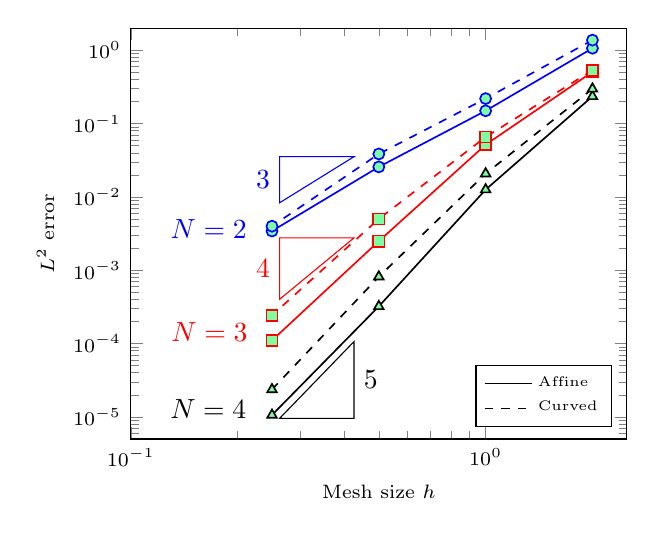
\begin{tikzpicture}
\begin{loglogaxis}[
    legend cell align=left,
    legend style={legend pos=south east, font=\tiny},
    width=.65\textwidth,    
    xlabel={Mesh size $h$},
    ylabel={$L^2$ error}, 
     ymin=5e-6, ymax=2,    
     xmin=1e-1, xmax=2.5,         
    grid style=dashed,
    legend entries={Affine,Curved}
] 
\addlegendimage{no markers,black}
\addlegendimage{no markers,dashed,black}

\addplot[color=blue,mark=*,semithick, mark options={solid,fill=markercolor}]
coordinates{(2,1.06717)(1,0.149639)(0.5,0.025693)(0.25,0.00342827)} [yshift=4pt] node[left, pos=1.05, color=blue] {$N = 2$};
\addplot[color=blue,mark=*,dashed,semithick, mark options={solid,fill=markercolor}]
coordinates{(2,1.37709)(1,0.219501)(0.5,0.0385896)(0.25,0.0039906)};
\logLogSlopeTriangleFlip{0.45}{0.15}{0.575}{3}{blue}


\addplot[color=red,mark=square*,semithick, mark options={solid,fill=markercolor}]
coordinates{(2,0.50782)(1,0.0516053)(0.5,0.00249425)(0.25,0.000110618)}[yshift=8pt] node[left, pos=1.05, color=red] {$N = 3$};
\addplot[color=red,mark=square*,dashed,semithick, mark options={solid,fill=markercolor}]
coordinates{(2,0.535036)(1,0.0657418)(0.5,0.00501536)(0.25,0.000243005)};
\logLogSlopeTriangleFlip{0.45}{0.15}{0.34}{4}{red}

\addplot[color=black,mark=triangle*,semithick, mark options={solid,fill=markercolor}]
coordinates{(2,0.235374)(1,0.0125714)(0.5,0.000321559)(0.25,1.06097e-05)} [yshift=8pt] node[left, pos=1.05, color=black] {$N = 4$};
\addplot[color=black,mark=triangle*,dashed,semithick, mark options={solid,fill=markercolor}]
coordinates{(2,0.297758)(1,0.0207604)(0.5,0.000816006)(0.25,2.36102e-05)};
\logLogSlopeTriangle{0.45}{0.15}{0.05}{5}{black}

%\legend{$L^2$ projection,Weight-adjusted,Difference}
%\legend{Uniform, Optimal, Smoothed}
\end{loglogaxis}
\end{tikzpicture}
\caption{$L^2$ errors at $T=5$ for the 2D isentropic vortex on affine, curved meshes.}
}
\end{figure}
\only<1>{
\begin{itemize}
\item All experiments utilize weight-adjusted mass matrices.
\item Modified conservative variables $\tilde{\bm{u}} = \bm{u}\LRp{\tilde{\bm{v}}}$, $\tilde{\bm{v}} = \tilde{P}_N^k\bm{v}(\bm{u}_h)$ defined using weight-adjusted projection $\tilde{P}^k_N$.
\end{itemize}
}
}

\frame{
\frametitle{2D curved meshes: conservation of entropy}

\begin{figure}
\centering
\subfloat[With weight-adjusted projection]{
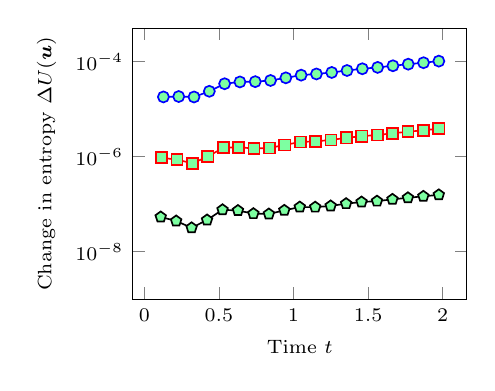
\begin{tikzpicture}
\begin{semilogyaxis}[
    legend cell align=left,
    legend style={legend pos=south east, font=\tiny},
    width=.48\textwidth,    
    xlabel={Time $t$},
    ylabel={Change in entropy $\Delta U(\bm{u})$}, 
     ymin=1e-9, ymax=5e-4,    
    grid style=dashed,
] 

\addplot[color=blue,mark=*,semithick, mark options={solid,fill=markercolor}]
coordinates{(0.025641,0)(0.128205,1.81455e-05)(0.230769,1.84993e-05)(0.333333,1.81016e-05)(0.435897,2.38212e-05)(0.538462,3.43804e-05)(0.641026,3.75077e-05)(0.74359,3.80509e-05)(0.846154,4.02406e-05)(0.948718,4.57864e-05)(1.05128,5.21023e-05)(1.15385,5.52339e-05)(1.25641,5.93653e-05)(1.35897,6.53204e-05)(1.46154,7.10508e-05)(1.5641,7.58692e-05)(1.66667,8.21148e-05)(1.76923,8.86933e-05)(1.87179,9.52306e-05)(1.97436,0.000102832)};
%\addplot[color=blue,dashed,semithick, mark options={solid,fill=markercolor}]
%coordinates{(0.025641,9.95731e-16)(0.128205,4.11303e-15)(0.230769,1.09496e-14)(0.333333,1.86934e-14)(0.435897,1.8624e-14)(0.538462,4.82253e-14)(0.641026,2.80886e-14)(0.74359,3.34073e-14)(0.846154,3.41116e-14)(0.948718,1.12826e-14)(1.05128,1.02106e-14)(1.15385,7.27543e-15)(1.25641,3.21965e-15)(1.35897,2.70617e-15)(1.46154,2.28116e-15)(1.5641,1.01134e-14)(1.66667,9.05179e-15)(1.76923,8.96852e-15)(1.87179,2.69368e-14)(1.97436,1.20043e-15)};
\addplot[color=red,mark=square*,semithick, mark options={solid,fill=markercolor}]
coordinates{(0.0129032,0)(0.116129,9.54018e-07)(0.219355,8.64409e-07)(0.322581,7.28292e-07)(0.425806,1.00547e-06)(0.529032,1.54507e-06)(0.632258,1.58376e-06)(0.735484,1.48926e-06)(0.83871,1.52599e-06)(0.941935,1.77263e-06)(1.04516,2.04306e-06)(1.14839,2.10785e-06)(1.25161,2.25231e-06)(1.35484,2.49471e-06)(1.45806,2.7075e-06)(1.56129,2.86391e-06)(1.66452,3.11015e-06)(1.76774,3.35711e-06)(1.87097,3.6045e-06)(1.97419,3.88568e-06)};
%\addplot[color=red,dotted,semithick, mark options={solid,fill=markercolor}]
%coordinates{(0.0129032,1.00787e-15)(0.116129,2.48065e-16)(0.219355,8.43769e-15)(0.322581,1.07483e-14)(0.425806,6.18255e-15)(0.529032,4.95159e-14)(0.632258,1.19835e-14)(0.735484,3.68837e-14)(0.83871,2.35957e-14)(0.941935,1.19904e-14)(1.04516,1.73785e-14)(1.14839,7.88952e-15)(1.25161,2.44249e-14)(1.35484,6.38031e-15)(1.45806,1.78781e-14)(1.56129,5.72459e-16)(1.66452,4.02456e-15)(1.76774,1.7316e-14)(1.87097,2.50425e-14)(1.97419,3.55375e-14)};
\addplot[color=black,mark=pentagon*,semithick, mark options={solid,fill=markercolor}]
coordinates{(0.00647249,0)(0.110032,5.38994e-08)(0.213592,4.43651e-08)(0.317152,3.18878e-08)(0.420712,4.65967e-08)(0.524272,7.64772e-08)(0.627832,7.36288e-08)(0.731392,6.33475e-08)(0.834951,6.22881e-08)(0.938511,7.43794e-08)(1.04207,8.71374e-08)(1.14563,8.67872e-08)(1.24919,9.19998e-08)(1.35275,1.02781e-07)(1.45631,1.11204e-07)(1.55987,1.16121e-07)(1.66343,1.26634e-07)(1.76699,1.36562e-07)(1.87055,1.46567e-07)(1.97411,1.57581e-07)};
%\addplot[color=black,dashdotted,semithick, mark options={solid,fill=markercolor}]
%coordinates{(0.00647249,2.19226e-16)(0.110032,5.88071e-15)(0.213592,1.34059e-14)(0.317152,2.30337e-14)(0.420712,8.23647e-15)(0.524272,2.68709e-14)(0.627832,2.53304e-14)(0.731392,2.95527e-14)(0.834951,2.5948e-14)(0.938511,4.56579e-15)(1.04207,2.28428e-14)(1.14563,8.22259e-15)(1.24919,1.51094e-14)(1.35275,7.86871e-15)(1.45631,1.11508e-14)(1.55987,1.57721e-14)(1.66343,6.95624e-15)(1.76699,2.07681e-14)(1.87055,2.72421e-14)(1.97411,1.7028e-14)};

% % N = 4, K= 8, dt = .25
 % N = 4, K= 8, dt = .125
 % N = 4, K= 8, dt = .0625

%\legend{${\rm CFL} = .25$,${\rm CFL} = .125$,${\rm CFL} = .0625$ }
%\legend{Uniform, Optimal, Smoothed}
\end{semilogyaxis}
\end{tikzpicture}
}
\subfloat[Without weight-adjusted projection]{
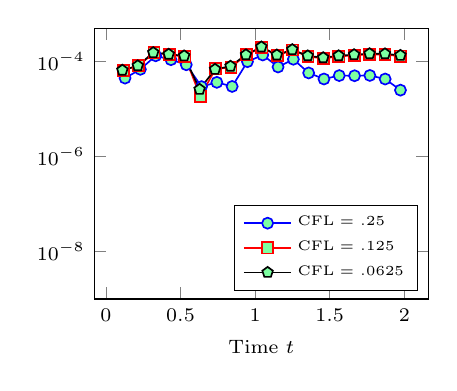
\begin{tikzpicture}
\begin{semilogyaxis}[
    legend cell align=left,
    legend style={legend pos=south east, font=\tiny},
    width=.48\textwidth,
    xlabel={Time $t$},
%         ymin=1e-10, ymax=1e-1,    
%     ymin=1e-7, ymax=1e1,
     ymin=1e-9, ymax=5e-4,    
%    ylabel={$L^2$ error}, 
    grid style=dashed,
] 

\addplot[color=blue,mark=*,semithick, mark options={solid,fill=markercolor}]
coordinates{(0.025641,0)(0.128205,4.45681e-05)(0.230769,6.82313e-05)(0.333333,0.000131517)(0.435897,0.000108761)(0.538462,8.51562e-05)(0.641026,2.94791e-05)(0.74359,3.62904e-05)(0.846154,2.97564e-05)(0.948718,9.87886e-05)(1.05128,0.000136806)(1.15385,7.64601e-05)(1.25641,0.000111044)(1.35897,5.72761e-05)(1.46154,4.27e-05)(1.5641,5.03819e-05)(1.66667,4.99789e-05)(1.76923,5.07438e-05)(1.87179,4.26361e-05)(1.97436,2.48694e-05)};
%\addplot[color=blue,dashed,semithick, mark options={solid,fill=markercolor}]
%coordinates{(0.025641,5.11743e-16)(0.128205,1.16547e-14)(0.230769,7.91034e-15)(0.333333,1.28231e-14)(0.435897,4.79131e-15)(0.538462,3.44134e-14)(0.641026,6.92502e-15)(0.74359,2.28047e-14)(0.846154,2.15314e-14)(0.948718,4.36456e-15)(1.05128,2.09416e-14)(1.15385,4.86763e-15)(1.25641,3.59088e-15)(1.35897,3.43475e-16)(1.46154,1.03632e-14)(1.5641,1.03598e-14)(1.66667,1.83881e-16)(1.76923,5.94663e-15)(1.87179,3.18252e-14)(1.97436,1.88495e-14)};
\addplot[color=red,mark=square*,semithick, mark options={solid,fill=markercolor}]
coordinates{(0.0129032,0)(0.116129,6.48664e-05)(0.219355,8.24474e-05)(0.322581,0.000152373)(0.425806,0.000138342)(0.529032,0.000126709)(0.632258,1.85501e-05)(0.735484,6.98555e-05)(0.83871,7.53129e-05)(0.941935,0.00013915)(1.04516,0.000196476)(1.14839,0.000133645)(1.25161,0.000173751)(1.35484,0.000126668)(1.45806,0.000116008)(1.56129,0.000127919)(1.66452,0.0001343)(1.76774,0.000140992)(1.87097,0.00013971)(1.97419,0.0001291)};
%\addplot[color=red,dotted,semithick, mark options={solid,fill=markercolor}]
%coordinates{(0.0129032,3.00107e-16)(0.116129,6.93196e-15)(0.219355,1.00198e-14)(0.322581,7.79932e-15)(0.425806,2.48759e-15)(0.529032,3.46181e-14)(0.632258,1.7205e-14)(0.735484,2.30718e-14)(0.83871,3.0146e-14)(0.941935,9.4369e-15)(1.04516,1.07969e-14)(1.14839,5.59275e-15)(1.25161,5.34295e-15)(1.35484,5.7801e-15)(1.45806,8.74648e-15)(1.56129,1.24137e-14)(1.66452,2.95597e-15)(1.76774,2.64441e-14)(1.87097,2.58023e-14)(1.97419,6.984e-15)};
\addplot[color=black,mark=pentagon*,semithick, mark options={solid,fill=markercolor}]
coordinates{(0.00647249,0)(0.110032,6.52844e-05)(0.213592,8.08628e-05)(0.317152,0.000153077)(0.420712,0.000141625)(0.524272,0.000130883)(0.627832,2.58046e-05)(0.731392,6.81127e-05)(0.834951,7.92926e-05)(0.938511,0.000137768)(1.04207,0.000201777)(1.14563,0.000136705)(1.24919,0.000177364)(1.35275,0.000131153)(1.45631,0.000119851)(1.55987,0.000131686)(1.66343,0.000138676)(1.76699,0.00014539)(1.87055,0.000144608)(1.97411,0.000134142)};
%\addplot[color=black,dashdotted,semithick, mark options={solid,fill=markercolor}]
%coordinates{(0.00647249,7.31403e-16)(0.110032,1.05055e-14)(0.213592,2.58127e-15)(0.317152,1.04916e-14)(0.420712,5.12437e-15)(0.524272,4.40203e-14)(0.627832,1.147e-14)(0.731392,2.81025e-14)(0.834951,3.01946e-14)(0.938511,4.51028e-15)(1.04207,1.096e-14)(1.14563,6.11317e-15)(1.24919,3.69843e-15)(1.35275,6.47399e-15)(1.45631,9.41608e-15)(1.55987,1.58901e-15)(1.66343,6.39766e-15)(1.76699,1.56819e-14)(1.87055,2.11949e-14)(1.97411,1.12063e-14)};

%\legend{Geo-$(N+1)$, $h^{N+2}$, Geo-$N$, $h^{N+1}$}
\legend{${\rm CFL} = .25$,${\rm CFL} = .125$,${\rm CFL} = .0625$ }
\end{semilogyaxis}
\end{tikzpicture}
}
%\subfloat[Convergence of $\Delta S(\bm{u})$]{
%\begin{tikzpicture}
%\begin{loglogaxis}[
%    legend cell align=left,
%    legend style={legend pos=south east, font=\tiny},
%    width=.475\textwidth,    
%    xlabel={Mesh size $h$},
%    ylabel={$L^2$ error}, 
%     ymin=5e-6, ymax=2,    
%     xmin=1e-1, xmax=2.5,         
%    grid style=dashed,
%    legend entries={Affine,Curved}
%] 
%\addlegendimage{no markers,black}
%\addlegendimage{no markers,dashed,black}
%
%\addplot[color=blue,mark=*,semithick, mark options={solid,fill=markercolor}]
%coordinates{(2,1.06717)(1,0.149639)(0.5,0.025693)(0.25,0.00342827)} [yshift=4pt] node[left, pos=1.05, color=blue] {$N = 2$};
%\logLogSlopeTriangleFlip{0.45}{0.15}{0.575}{3}{blue}
%
%
%%\legend{$L^2$ projection,Weight-adjusted,Difference}
%%\legend{Uniform, Optimal, Smoothed}
%\end{loglogaxis}
%\end{tikzpicture}
%}
\caption{Change in entropy under an entropy conservative flux with $N=4$.  In both cases, the spatial formulation tested with $\tilde{\bm{v}} = P_N\bm{v}(\bm{u})$ is $O\LRp{10^{-14}}$. }
%\label{fig:dSconverge}
\end{figure}
}

\frame{
\frametitle{3D isentropic vortex} 
\begin{figure}
\centering
\subfloat[Affine mesh for $h = 1/2$]{\raisebox{2em}{\includegraphics[width=.425\textwidth]{figs/periodicCube3.png}}\label{subfig:mesh3d}}
\subfloat[$L^2$ errors]{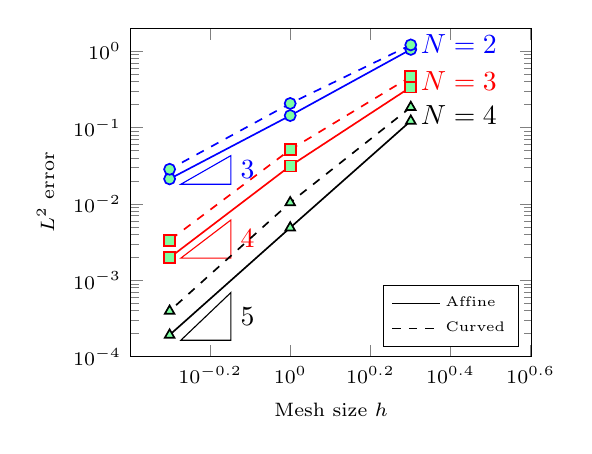
\begin{tikzpicture}
\begin{loglogaxis}[
    legend cell align=left,
    legend style={legend pos=south east, font=\tiny},
    width=.55\textwidth,    
    xlabel={Mesh size $h$},
    ylabel={$L^2$ error}, 
     ymin=1e-4, ymax=2,    
     xmin=4e-1, xmax=4,         
    grid style=dashed,
    legend entries={Affine,Curved}
] 
\addlegendimage{no markers,black}
\addlegendimage{no markers,dashed,black}

\addplot[color=blue,mark=*,semithick, mark options={solid,fill=markercolor}]
coordinates{(2,1.05519)(1,0.143515)(0.5,0.0212682)}[yshift=2pt] node[right, pos=.0, color=blue] {$N = 2$};
\addplot[color=blue,mark=*,dashed,semithick, mark options={solid,fill=markercolor}]
coordinates{(2,1.20915)(1,0.2069)(0.5,0.0284505)};
\logLogSlopeTriangle{0.25}{0.125}{0.525}{3}{blue}

\addplot[color=red,mark=square*,semithick, mark options={solid,fill=markercolor}]
coordinates{(2,0.339318)(1,0.0314342)(0.5,0.00197699)}[yshift=2pt] node[right, pos=0, color=red] {$N = 3$};
\addplot[color=red,mark=square*,dashed,semithick, mark options={solid,fill=markercolor}]
coordinates{(2,0.464613)(1,0.0513369)(0.5,0.00334595)};
\logLogSlopeTriangle{0.25}{0.125}{0.3}{4}{red}

\addplot[color=black,mark=triangle*,semithick, mark options={solid,fill=markercolor}]
coordinates{(2,0.122229)(1,0.00488434)(0.5,0.000192453)}[yshift=2pt] node[right, pos=0, color=black] {$N = 4$};
\addplot[color=black,mark=triangle*,dashed,semithick, mark options={solid,fill=markercolor}]
coordinates{(2,0.184547)(1,0.0104361)(.5,0.0003960681)};
\logLogSlopeTriangle{0.25}{0.125}{0.05}{5}{black}

%\legend{$L^2$ projection,Weight-adjusted,Difference}
%\legend{Uniform, Optimal, Smoothed}
\end{loglogaxis}
\end{tikzpicture}}
\caption{$L^2$ errors at $T=5$ for the 3D isentropic vortex on affine, curved meshes.}
\label{fig:converge3d}
\end{figure}
}


\frame{
\frametitle{ Taylor-Green vortex} 
%\vspace{-1em}
\begin{figure}
\centering
\includegraphics[width=.65\textwidth]{figs/taylorgreen.png}
\caption{Isocontours of $z$-vorticity for Taylor-Green at $t = 0, 10$ seconds.}
\end{figure}
%\vspace{-.5em}
\begin{itemize}
\item Simple turbulence-like behavior (generation of small scales).
%\vspace{.25em}
\item Inviscid Taylor-Green: tests robustness w.r.t.\ under-resolved solutions.
\end{itemize}
\let\thefootnote\relax\footnotetext{\tiny \url{https://how4.cenaero.be/content/bs1-dns-taylor-green-vortex-re1600}.}
}

\frame{
\frametitle{Taylor-Green vortex: kinetic energy dissipation rate} 

\begin{figure}
%\centering
\subfloat[Kinetic energy ]{
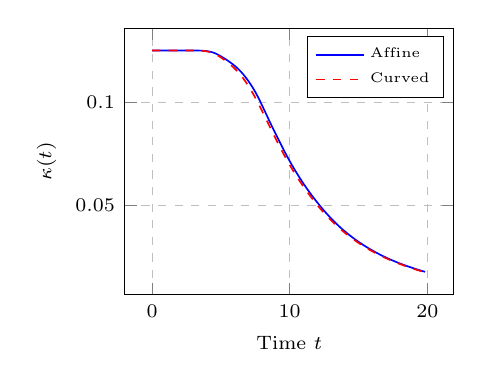
\begin{tikzpicture}
\begin{axis}[
        scaled ticks=false, 
        tick label style={/pgf/number format/fixed},
	legend cell align=left,
	legend style={font=\tiny},
	width=.475\textwidth,
    xlabel={Time $t$},
    ylabel={$\kappa(t)$},
%    xmin=.005, xmax=1,
%    ymin=1e-10, ymax=1e-1,
    legend pos=north east,
    xmajorgrids=true,
    ymajorgrids=true,
    grid style=dashed,
%    ytick={0,.001, .005, .01, .015},
%    yticklabels={$0$,$\frac{\pi}{2}$,$\pi$,$\frac{3\pi}{2}$},
] 
\addplot[color=blue,,semithick, mark options={fill=markercolor}]
coordinates{(0,0.125)(0.178731,0.125)(0.357462,0.125002)(0.536193,0.125005)(0.714924,0.125009)(0.893655,0.125014)(1.07239,0.125018)(1.25112,0.125023)(1.42985,0.125027)(1.60858,0.125031)(1.78731,0.125034)(1.96604,0.125037)(2.14477,0.125039)(2.3235,0.12504)(2.50223,0.125039)(2.68097,0.125037)(2.8597,0.125032)(3.03843,0.125023)(3.21716,0.125008)(3.39589,0.124984)(3.57462,0.124942)(3.75335,0.124872)(3.93208,0.124756)(4.11081,0.124577)(4.28954,0.124315)(4.46828,0.123948)(4.64701,0.123461)(4.82574,0.122861)(5.00447,0.122182)(5.1832,0.12146)(5.36193,0.120701)(5.54066,0.119905)(5.71939,0.119069)(5.89812,0.118168)(6.07685,0.117182)(6.25558,0.1161)(6.43432,0.1149)(6.61305,0.113564)(6.79178,0.112093)(6.97051,0.110495)(7.14924,0.108768)(7.32797,0.106898)(7.5067,0.104859)(7.68543,0.10263)(7.86416,0.100247)(8.04289,0.0977593)(8.22163,0.0952161)(8.40036,0.092669)(8.57909,0.0901535)(8.75782,0.0876812)(8.93655,0.0852575)(9.11528,0.0828687)(9.29401,0.0804991)(9.47274,0.0781493)(9.65147,0.0758373)(9.83021,0.0735985)(10.0089,0.0714455)(10.1877,0.0693647)(10.3664,0.0673466)(10.5451,0.0653915)(10.7239,0.063496)(10.9026,0.0616565)(11.0813,0.0598745)(11.2601,0.0581523)(11.4388,0.0564894)(11.6175,0.0548814)(11.7962,0.0533217)(11.975,0.0518057)(12.1537,0.0503292)(12.3324,0.0488935)(12.5112,0.0475009)(12.6899,0.0461529)(12.8686,0.0448499)(13.0474,0.0435915)(13.2261,0.0423768)(13.4048,0.0412054)(13.5836,0.0400793)(13.7623,0.0390016)(13.941,0.0379701)(14.1197,0.0369793)(14.2985,0.0360246)(14.4772,0.0351027)(14.6559,0.0342115)(14.8347,0.0333479)(15.0134,0.032511)(15.1921,0.0317027)(15.3709,0.0309235)(15.5496,0.0301727)(15.7283,0.0294487)(15.9071,0.0287493)(16.0858,0.0280732)(16.2645,0.027421)(16.4433,0.0267929)(16.622,0.0261868)(16.8007,0.0256001)(16.9794,0.025031)(17.1582,0.0244798)(17.3369,0.023947)(17.5156,0.0234321)(17.6944,0.0229344)(17.8731,0.0224536)(18.0518,0.0219896)(18.2306,0.0215416)(18.4093,0.0211082)(18.588,0.0206882)(18.7668,0.02028)(18.9455,0.0198829)(19.1242,0.0194966)(19.3029,0.0191212)(19.4817,0.0187558)(19.6604,0.0184)(19.8391,0.0180542)};

\addplot[color=red,dashed,semithick, mark options={fill=markercolor}]
coordinates{(0,0.125)(0.18796,0.125)(0.37592,0.125002)(0.563879,0.125006)(0.751839,0.125009)(0.939799,0.125014)(1.12776,0.125019)(1.31572,0.125024)(1.50368,0.125028)(1.69164,0.125032)(1.8796,0.125035)(2.06756,0.125037)(2.25552,0.125038)(2.44348,0.125036)(2.63144,0.125032)(2.8194,0.125023)(3.00736,0.125009)(3.19532,0.124985)(3.38328,0.124947)(3.57124,0.124884)(3.7592,0.124781)(3.94716,0.124621)(4.13512,0.124379)(4.32308,0.124027)(4.51104,0.123541)(4.699,0.122909)(4.88696,0.122149)(5.07491,0.121302)(5.26288,0.120396)(5.45083,0.11944)(5.6388,0.118433)(5.82676,0.11736)(6.01471,0.116193)(6.20267,0.114912)(6.39063,0.113497)(6.57859,0.11193)(6.76655,0.110204)(6.95451,0.108334)(7.14247,0.106322)(7.33043,0.104189)(7.51839,0.101934)(7.70635,0.0995426)(7.89431,0.0970654)(8.08227,0.0945369)(8.27023,0.0919787)(8.45819,0.0894304)(8.64615,0.0868905)(8.83411,0.0843671)(9.02207,0.0818692)(9.21003,0.0794052)(9.39799,0.0769825)(9.58595,0.0746288)(9.77391,0.0723431)(9.96187,0.0701295)(10.1498,0.0679956)(10.3378,0.0659364)(10.5258,0.0639473)(10.7137,0.0620322)(10.9017,0.0601792)(11.0896,0.0583829)(11.2776,0.0566368)(11.4656,0.0549345)(11.6535,0.053277)(11.8415,0.0516697)(12.0294,0.0501198)(12.2174,0.0486301)(12.4053,0.047197)(12.5933,0.0458163)(12.7813,0.0444834)(12.9692,0.0431979)(13.1572,0.0419597)(13.3451,0.0407697)(13.5331,0.0396274)(13.7211,0.038527)(13.909,0.0374678)(14.097,0.0364487)(14.2849,0.0354663)(14.4729,0.034518)(14.6609,0.0336038)(14.8488,0.0327232)(15.0368,0.0318737)(15.2247,0.0310535)(15.4127,0.0302625)(15.6007,0.0295011)(15.7886,0.0287685)(15.9766,0.0280626)(16.1645,0.0273818)(16.3525,0.0267242)(16.5405,0.0260884)(16.7284,0.0254745)(16.9164,0.0248826)(17.1043,0.0243113)(17.2923,0.0237595)(17.4803,0.0232271)(17.6682,0.0227134)(17.8562,0.0222159)(18.0441,0.0217324)(18.2321,0.0212626)(18.4201,0.0208084)(18.608,0.0203709)(18.796,0.019949)(18.9839,0.0195411)(19.1719,0.0191457)(19.3599,0.0187618)(19.5478,0.0183882)(19.7358,0.0180246)(19.9237,0.0176713)};

\legend{Affine, Curved}
\end{axis}\end{tikzpicture}
}
\hspace{.25em}
\subfloat[Kinetic energy dissipation rate]{
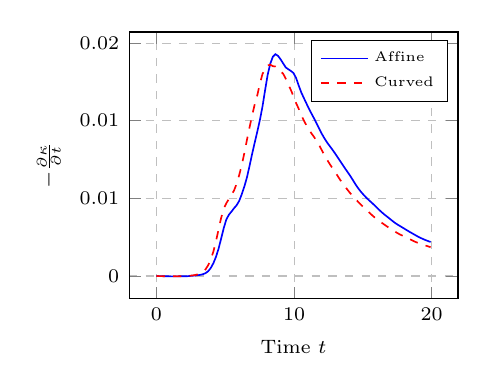
\begin{tikzpicture}
\begin{axis}[
        scaled ticks=false, 
        tick label style={/pgf/number format/fixed},
	legend cell align=left,
	legend style={font=\tiny},
	width=.475\textwidth,
    xlabel={Time $t$},
    ylabel={$-\pd{\kappa}{t}$},
%    xmin=.005, xmax=1,
%    ymin=1e-10, ymax=1e-1,
    legend pos=north east,
    xmajorgrids=true,
    ymajorgrids=true,
    grid style=dashed,
%    ytick={0, .005, .01, .015},
%    yticklabels={0, .005, .01, .015}    
] 
\addplot[color=blue,semithick, mark options={fill=markercolor}]
coordinates{(0,-0)(0.18796,-8.45875e-06)(0.37592,-9.02267e-06)(0.563879,-1.63536e-05)(0.751839,-1.40979e-05)(0.939799,-2.48123e-05)(1.12776,-2.65041e-05)(1.31572,-2.76319e-05)(1.50368,-2.53763e-05)(1.69164,-2.0301e-05)(1.8796,-2.31206e-05)(2.06756,-1.69175e-05)(2.25552,-1.3534e-05)(2.44348,2.25567e-06)(2.63144,1.63536e-05)(2.8194,2.98876e-05)(3.00736,4.90608e-05)(3.19532,7.38731e-05)(3.38328,0.000117859)(3.57124,0.000183837)(3.7592,0.000306771)(3.94716,0.000514292)(4.13512,0.000819935)(4.32308,0.00122765)(4.51104,0.00175378)(4.699,0.00240454)(4.88696,0.00307729)(5.07491,0.00363332)(5.26288,0.00394291)(5.45083,0.00414817)(5.6388,0.00436754)(5.82676,0.00455927)(6.01471,0.00484235)(6.20267,0.00527544)(6.39063,0.00577169)(6.57859,0.0063638)(6.76655,0.00709971)(6.95451,0.00787679)(7.14247,0.00860142)(7.33043,0.0093097)(7.51839,0.0100575)(7.70635,0.0109236)(7.89431,0.011972)(8.08227,0.0129661)(8.27023,0.013675)(8.45819,0.0141244)(8.64615,0.0142863)(8.83411,0.0141814)(9.02207,0.0139541)(9.21003,0.0136913)(9.39799,0.0134325)(9.58595,0.0133152)(9.77391,0.0132047)(9.96187,0.0130733)(10.1498,0.0127473)(10.3378,0.0122686)(10.5258,0.0118191)(10.7137,0.0114588)(10.9017,0.011108)(11.0896,0.0107578)(11.2776,0.0104415)(11.4656,0.0101274)(11.6535,0.00979918)(11.8415,0.00946253)(12.0294,0.00913827)(12.2174,0.00885124)(12.4053,0.00859409)(12.5933,0.00836514)(12.7813,0.00814465)(12.9692,0.00790724)(13.1572,0.00766025)(13.3451,0.00740818)(13.5331,0.0071578)(13.7211,0.00691137)(13.909,0.00667057)(14.097,0.0064264)(14.2849,0.00616305)(14.4729,0.0058918)(14.6609,0.00565045)(14.8488,0.00543559)(15.0368,0.00524499)(15.2247,0.00506736)(15.4127,0.00490326)(15.6007,0.00475551)(15.7886,0.00460156)(15.9766,0.00443803)(16.1645,0.00427562)(16.3525,0.00412054)(16.5405,0.00397618)(16.7284,0.00384422)(16.9164,0.00371339)(17.1043,0.00357805)(17.2923,0.00344835)(17.4803,0.00333275)(17.6682,0.00323237)(17.8562,0.00313369)(18.0441,0.00303105)(18.2321,0.00292842)(18.4201,0.00282973)(18.608,0.00273556)(18.796,0.00264082)(18.9839,0.00254834)(19.1719,0.00246319)(19.3599,0.0023848)(19.5478,0.00231431)(19.7358,0.00225059)(19.9237,0.00218969)};

\addplot[color=red, dashed,semithick, mark options={fill=markercolor}]
coordinates{(0,5.36239e-07)(0.18796,-9.65229e-06)(0.37592,-1.01885e-05)(0.563879,-1.98408e-05)(0.751839,-1.76959e-05)(0.939799,-1.93046e-05)(1.12776,-2.14495e-05)(1.31572,-1.93046e-05)(1.50368,-2.4667e-05)(1.69164,-1.66234e-05)(1.8796,-8.57982e-06)(2.06756,-0)(2.25552,1.17972e-05)(2.44348,1.76959e-05)(2.63144,3.70005e-05)(2.8194,6.43486e-05)(3.00736,0.000107784)(3.19532,0.000173741)(3.38328,0.000268656)(3.57124,0.000432745)(3.7592,0.000693357)(3.94716,0.00106122)(4.13512,0.00156796)(4.32308,0.00222485)(4.51104,0.00299597)(4.699,0.00373597)(4.88696,0.00432584)(5.07491,0.00468404)(5.26288,0.00495645)(5.45083,0.00521599)(5.6388,0.00551361)(5.82676,0.0059426)(6.01471,0.00650672)(6.20267,0.00717005)(6.39063,0.00793258)(6.57859,0.00878681)(6.76655,0.0095858)(6.95451,0.0103457)(7.14247,0.0110685)(7.33043,0.0116551)(7.51839,0.0124011)(7.70635,0.013015)(7.89431,0.0133341)(8.08227,0.0135652)(8.27023,0.0136097)(8.45819,0.0135175)(8.64615,0.0134918)(8.83411,0.0133647)(9.02207,0.0131925)(9.21003,0.0130242)(9.39799,0.012703)(9.58595,0.0123292)(9.77391,0.011971)(9.96187,0.0115586)(10.1498,0.0111345)(10.3378,0.0107687)(10.5258,0.0103671)(10.7137,0.0100089)(10.9017,0.00969788)(11.0896,0.00941206)(11.2776,0.00916861)(11.4656,0.00893803)(11.6535,0.00868707)(11.8415,0.00840018)(12.0294,0.00807897)(12.2174,0.00776742)(12.4053,0.00747785)(12.5933,0.00721187)(12.7813,0.00696306)(12.9692,0.00670834)(13.1572,0.00645792)(13.3451,0.00619624)(13.5331,0.00595922)(13.7211,0.00574312)(13.909,0.00552219)(14.097,0.00531841)(14.2849,0.0051318)(14.4729,0.0049527)(14.6609,0.00476984)(14.8488,0.00459717)(15.0368,0.00443791)(15.2247,0.00428401)(15.4127,0.00412689)(15.6007,0.00396924)(15.7886,0.00382231)(15.9766,0.00368503)(16.1645,0.00355633)(16.3525,0.00343783)(16.5405,0.00332253)(16.7284,0.00320563)(16.9164,0.00309088)(17.1043,0.00298524)(17.2923,0.00288282)(17.4803,0.00277932)(17.6682,0.00268602)(17.8562,0.00260719)(18.0441,0.00253641)(18.2321,0.00245865)(18.4201,0.00237071)(18.608,0.0022833)(18.796,0.00220501)(18.9839,0.00213584)(19.1719,0.00207203)(19.3599,0.00201358)(19.5478,0.00196102)(19.7358,0.0019074)(19.9237,0.00185056)};

\legend{Affine, Curved}
\end{axis}\end{tikzpicture}
}
\caption{Evolution of kinetic energy $\kappa(t)$ and kinetic energy dissipation rate $-\pd{\kappa}{t}$ for $N=3, h = \pi/8, \text{CFL} = .25$ on affine and curved meshes of $[-\pi,\pi]^3$.}
\end{figure}
}


%% =================================================

\frame{
\frametitle{Summary and future work}

\begin{itemize}
\item Discretely stable time-domain discontinuous Galerkin methods: provable semi-discrete stability for high order methods.  
\vspace{.25em}
\item Additional work required: strong shocks, positivity preservation.  
\vspace{.25em}
\item Current work: hybrid meshes, continuous FEM, regularization (limiting, artificial viscosity), multi-GPU (with Lucas Wilcox).  
\vspace{.25em}
\item This work is supported by DMS-1719818. 
\end{itemize}
\vspace{.25em}
\begin{center}
Thank you!  Questions?
\vspace{.25em}

{\includegraphics[width=.15\textwidth]{figs/nsf.jpg}}
\end{center}


\let\thefootnote\relax\footnotetext{\tiny Chan, Wilcox (in preparation). \textit{On discretely entropy stable weight-adjusted DG methods: curvilinear meshes}.}
%\let\thefootnote\relax\footnotetext{\tiny Chan, Hewett, and Warburton (2016). \textit{Weight-adjusted discontinuous Galerkin methods: curvilinear meshes}.}
\let\thefootnote\relax\footnotetext{\tiny Chan (2017). \textit{On discretely entropy conservative and entropy stable discontinuous Galerkin methods.}}

}

%% =================================================


\begin{frame}[noframenumbering]
\frametitle{Additional slides }
\end{frame}




\frame[noframenumbering]{
\frametitle{Over-integration is ineffective without $L^2$ projection}

\begin{figure}[!h]
\centering
\begingroup
\captionsetup[subfigure]{width=.5\textwidth}
\subfloat[$(N+1)$ points]{\includegraphics[width=.45\textwidth]{figs/sbpGLL.png}}
\hspace{1em}
\subfloat[$(N+4)$ points]{\includegraphics[width=.45\textwidth]{figs/sbpGLLNp4.png}}
\endgroup
%\subfloat[$(N+4)$ point GLL]{\includegraphics[width=.32\textwidth]{figs/dsbpGLLNp4.png}}
\caption{Numerical results for the Sod shock tube for $N=4$ and $K=32$ elements.  Over-integrating by increasing the number of quadrature points does not improve solution quality.  }
\label{fig:sbpq}
\end{figure}
}

%
%\frame[noframenumbering]{
%\frametitle{Asymptotically non-affine geometric mappings}
%
%%\only<1-2>{
%%Comparison with $L^2$ projection and Low-Storage Curvilinear DG
%%\[
%%\tilde{\phi}_i = \frac{\phi_i}{\sqrt{J}}, \qquad \bm{M}_{ij} = \int_{D^k} \tilde{\phi}_j\tilde{\phi}_i J = \int_{\widehat{D}} \phi_j\phi_i = \widehat{\bm{M}}_{ij}.
%%\]
%%\vspace{-2em}
%%}
%
%\begin{figure}
%\begin{overlayarea}{\textwidth}{.6\textheight}
%\centering
%\only<1>{
%\vspace{-2em}
%Similar rate of convergence for both $L^2$ projection and WADG.
%\vspace{1em}
%
%\subfloat{
%\includegraphics[width=.37\textwidth]{figs/randunif1.png}
%}
%\subfloat{
%\begin{tikzpicture}
%\begin{loglogaxis}[
%	legend cell align=left,
%	        legend style={font=\tiny},
%	width=.49\textwidth,
%    xlabel={Mesh size $h$},
%    ylabel={$L^2$ error},
%    xmin=.005, xmax=1,
%    ymin=1e-10, ymax=1e-1,
%    legend pos=south east,
%    xmajorgrids=true,
%    ymajorgrids=true,
%    grid style=dashed,
%] 
%\addplot[color=blue,mark=*,mark size=3,semithick, mark options={fill=markercolor}]
%coordinates{(0.5,0.00943375)(0.25,0.00276313)(0.125,0.000415615)(0.0625,6.56974e-05)(0.03125,8.95162e-06)(0.015625,1.14109e-06)};
%%\addplot[color=black,mark=diamond*,mark size=4,semithick, mark options={fill=markercolor}]
%%coordinates{(0.5,0.0134065)(0.25,0.012209)(0.125,0.004612)(0.0625,0.00163555)(0.03125,0.000458367)(0.015625,0.00011822)};
%\addplot[color=red,mark=square*,mark size=3,semithick, mark options={fill=markercolor}]
%coordinates{(0.5,0.00990795)(0.25,0.00389737)(0.125,0.00064227)(0.0625,0.000123078)(0.03125,1.80455e-05)(0.015625,2.28866e-06)};
%\logLogSlopeTriangleFlip{0.325}{0.125}{0.525}{3}{red};
%\logLogSlopeTriangle{0.325}{0.125}{0.375}{3}{blue};
%
%%\legend{$L^2$ projection, LSC-DG, WADG}
%\legend{$L^2$ projection, WADG}
%\end{loglogaxis}
%\end{tikzpicture}
%}
%\caption{Curvilinear element constructed through random perturbation for $N = 3$.}
%}
%\only<2>{
%\vspace{-2em}
%High order convergence \textcolor{red}{slowed} by growth of $\nor{J}_{W^{N+1,\infty}} = O(h)$.
%\vspace{1em}
%
%\subfloat{
%\includegraphics[width=.37\textwidth]{figs/arnoldmesh1.png}
%}
%\subfloat{
%\begin{tikzpicture}
%\begin{loglogaxis}[
%	legend cell align=left,
%	        legend style={font=\tiny},	
%	width=.49\textwidth,
%    xlabel={Mesh size $h$},
%    ylabel={$L^2$ error},
%    xmin=.005, xmax=1,
%    ymin=1e-10, ymax=1e-1,
%    legend pos=south east,
%    xmajorgrids=true,
%    ymajorgrids=true,
%    grid style=dashed,
%] 
%% adding this 2x because pgfplots dashes the line for some reason...
%\addplot[color=blue,mark=*,mark size=3,semithick, mark options={fill=markercolor}]
%coordinates{(0.5,0.00145465)(0.25,0.000140693)(0.125,1.17949e-05)(0.0625,8.58138e-07)(0.03125,5.78543e-08)(0.015625,3.75483e-09)};
%%\addplot[color=black,mark=diamond*,mark size=4,semithick, mark options={fill=markercolor}]
%%coordinates{(0.5,0.00159198)(0.25,0.000658818)(0.125,0.000619747)(0.0625,0.000677173)(0.03125,0.00073964)(0.015625,0.000782687)};
%\addplot[color=red,mark=square*,mark size=3,semithick, mark options={fill=markercolor}]
%coordinates{(0.5,0.00148852)(0.25,0.000176325)(0.125,2.60169e-05)(0.0625,3.94602e-06)(0.03125,5.58752e-07)(0.015625,7.47639e-08)};
%\logLogSlopeTriangleFlip{0.325}{0.125}{0.37}{3}{red};
%\logLogSlopeTriangle{0.35}{0.125}{0.12}{4}{blue};
%
%%\legend{$L^2$ projection, LSC-DG, WADG}
%\legend{$L^2$ projection, WADG}
%\end{loglogaxis}
%\end{tikzpicture}
%}
%\caption{Arnold-type element with $\nor{J}_{W^{N+1,\infty}} = O(h^{-1})$ for $N = 3$.}
%}
%\only<3>{
%\vspace{-2em}
%High order convergence \textcolor{red}{slowed} by growth of $\nor{J}_{W^{N+1,\infty}} = O(h^{-N})$.
%\vspace{1em}
%
%\subfloat{
%\includegraphics[width=.37\textwidth]{figs/curvarnold2ref.png}
%}
%\subfloat{
%\begin{tikzpicture}
%\begin{loglogaxis}[
%legend style={font=\tiny},
%	legend cell align=left,
%	width=.49\textwidth,
%    xlabel={Mesh size $h$},
%    ylabel={$L^2$ error},
%    xmin=.0025, xmax=1,
%    ymin=1e-7, ymax=1e-0,
%    legend pos=south east,
%    xmajorgrids=true,
%    ymajorgrids=true,
%    grid style=dashed,
%] 
%% adding this 2x because pgfplots dashes the line for some reason...
%\addplot[color=blue,mark=*,mark size=3,semithick, mark options={fill=markercolor}]
%coordinates{(0.5,0.0149174)(0.25,0.00576658)(0.125,0.00165616)(0.0625,0.000433839)(0.03125,0.000110389)(0.015625,2.78024e-05)};
%%\addplot[color=black,mark=diamond*,mark size=4,semithick, mark options={fill=markercolor}]
%%coordinates{(0.5,0.018737)(0.25,0.0147278)(0.125,0.0117761)(0.0625,0.0110991)(0.03125,0.0112431)(0.015625,0.0114663)};
%\addplot[color=red,mark=square*,mark size=3,semithick, mark options={fill=markercolor}]
%coordinates{(0.5,0.0165783)(0.25,0.00872368)(0.125,0.00464969)(0.0625,0.00253621)(0.03125,0.00134518)(0.015625,0.000695124)};
%\logLogSlopeTriangleFlip{0.41}{0.15}{0.6}{1}{red};
%\logLogSlopeTriangle{0.41}{0.15}{0.25}{2}{blue};
%
%%\node at (axis cs:.03,2.1e-07) {$a = 10^{-1}$};
%
%%\legend{$L^2$ proj, LSC-DG, WADG}
%\legend{$L^2$ proj, WADG}
%\end{loglogaxis}
%\end{tikzpicture}
%}
%\caption{Moderately warped curved Arnold-type element for $N = 3$.}
%}
%\only<4>{
%\vspace{-2em}
%High order convergence is \textcolor{red}{stalled} by growth of $\nor{J}_{W^{N+1,\infty}} = O(h^{-(N+1)})$.
%\vspace{1em}
%
%\subfloat{
%\includegraphics[width=.37\textwidth]{figs/curvarnold1ref.png}
%}
%\subfloat{
%\begin{tikzpicture}
%\begin{loglogaxis}[
%legend style={font=\tiny},
%	legend cell align=left,
%	width=.49\textwidth,
%    xlabel={Mesh size $h$},
%    ylabel={$L^2$ error},
%    xmin=.0025, xmax=1,
%    ymin=1e-7, ymax=1e-0,
%    legend pos=south east,
%    xmajorgrids=true,
%    ymajorgrids=true,
%    grid style=dashed,
%] 
%\addplot[color=blue,mark=*,mark size=3,semithick, mark options={fill=markercolor}]
%coordinates{(0.5,0.038232)(0.25,0.0144542)(0.125,0.00400233)(0.0625,0.000991275)(0.03125,0.000234827)(0.015625,5.4896e-05)};
%%\addplot[color=black,mark=diamond*,mark size=4,semithick, mark options={fill=markercolor}]
%%coordinates{(0.5,0.0579895)(0.25,0.052133)(0.125,0.0462352)(0.0625,0.0434683)(0.03125,0.0394193)(0.015625,0.032696)};
%\addplot[color=red,mark=square*,mark size=3,semithick, mark options={fill=markercolor}]
%coordinates{(0.5,0.0681969)(0.25,0.0751338)(0.125,0.0744307)(0.0625,0.0695447)(0.03125,0.0656228)(0.015625,0.0653247)};
%%\logLogSlopeTriangleFlip{0.3}{0.125}{0.475}{1}{red};
%\logLogSlopeTriangleFlip{0.425}{0.15}{0.45}{2}{blue};
%
%%\node at (axis cs:.03,2.1e-07) {$a = 10^{-1}$};
%
%%\legend{$L^2$ proj, LSC-DG, WADG}
%\legend{$L^2$ proj, WADG}
%\end{loglogaxis}
%\end{tikzpicture}
%}
%\caption{Heavily warped curved Arnold-type element for $N = 3$.}
%}
%
%\end{overlayarea}
%
%\end{figure}
%}
%
%\frame[noframenumbering]{
%\frametitle{Weight-adjusted DG: local conservation}
%
%\begin{itemize}
%\item \textcolor{red}{Con:} loss of local conservation for $w(x) \not\in P^N$!
%\vspace{1em}
%\item \textcolor{blue}{Pro:} superconvergence of conservation error
%\begin{align*}
%&\LRb{\int_{\widehat{D}} w p(\bm{x},t) - \int_{\widehat{D}} T_{1/w}^{-1} p(\bm{x},t)} \\
%\text{Conservation error}
%&\leq C \textcolor{red}{h^{2N+2}} \nor{w}_{W^{N+1,\infty}}\nor{p}_{W^{N+1,2}}
%\end{align*}
%where $C$ depends on mesh quality and max/min values of $w$.
%\vspace{1em}
%\item \textcolor{blue}{Pro:} can restore local conservation with rank-1 update (Shermann-Morrison).
%\end{itemize}
%}
%
%
%\frame[noframenumbering]{
%\frametitle{Effect of conservation on shock speeds}
%
%\begin{itemize}
%\item Weighted Burgers' equation, $w(x)$ curves characteristic lines.
%\[
%w(x)\pd{u}{t}{} + \frac{1}{2}\pd{u^2}{x}{} = 0.
%\]
%\item WADG yields high order convergence, correct shock speed for both $w(x)$ smooth, discontinuous (within an element).
%\end{itemize}
%%\vspace{-1em}
%\begin{overlayarea}{\textwidth}{.55\textheight}
%\only<1>{
%\begin{figure}
%\centering
%\subfloat[Smooth solution]{\includegraphics[width=.4\textwidth]{figs/burgersSmooth2.png}}
%\hspace{1em}
%\subfloat[Shock solution]{\includegraphics[width=.39\textwidth]{figs/burgersShock2.png}}
%\end{figure}
%}
%\only<2>{
%\vspace{2em}
%\begin{center}
%Best guess: {where} and {what} is locally conserved matters;\\ non-conservation of \textit{nonlinear flux} results in incorrect shock speeds.  
%\end{center}
%}
%\end{overlayarea}
%}


\bibliographystyle{plain}
{\scriptsize
\bibliography{pyramids}
}

\end{document}
